\documentclass[a4paper,german]{article}
%Mainly taken from
%https://github.com/gillescastel/university-setup/blob/master/preamble.tex
%but edited for own purposes

%%%%%OWN
%%Own basic packages
\usepackage{mkessler-math}
\usepackage{mkessler-fancythm}
\usepackage{mkessler-operators}

\usepackage{datetime}
\date{{\normalfont Mitschrift}\\{\sc Maximilian Keßler}}

\usepackage{wrapfig}
\usepackage{pgfplots}
\pgfplotsset{compat=1.7}
%%%%%%Preamble from Gilles Castel
% Some basic packages
\usepackage{url}
\usepackage{graphicx}
\usepackage{float}

% for wrapping text around figures
\usepackage{wrapfig}

%%This option is for now commented out, not sure what it does, but causes errors
%\pdfminorversion=7


% Don't indent paragraphs, leave some space between them
\usepackage{parskip}

% Hide page number when page is empty
\usepackage{emptypage}
% Other font I sometimes use.
\usepackage{xcolor}
% \usepackage{cmbright}

% Math stuff
\usepackage{amsfonts}

% Put x \to \infty below \lim
\let\svlim\lim\def\lim{\svlim\limits}

%Make implies and impliedby shorter
\let\implies\Rightarrow
\let\impliedby\Leftarrow
\let\iff\Leftrightarrow
\let\epsilon\varepsilon

% Command for short corrections
% Usage: 1+1=\correct{3}{2}

% Environments
\makeatother

% Fix some spacing
% http://tex.stackexchange.com/questions/22119/how-can-i-change-the-spacing-before-theorems-with-amsthm
\makeatletter
\def\thm@space@setup{%
  \thm@preskip=\parskip \thm@postskip=0pt
}


% \lecture starts a new lecture (les in dutch)
%
% Usage:
% \lecture{1}{di 12 feb 2019 16:00}{Inleiding}
%
% This adds a section heading with the number / title of the lecture and a
% margin paragraph with the date.

% I use \dateparts here to hide the year (2019). This way, I can easily parse
% the date of each lecture unambiguously while still having a human-friendly
% short format printed to the pdf.

\usepackage{xifthen}
\def\testdateparts#1{\dateparts#1\relax}
\def\dateparts#1 #2 #3 #4 #5\relax{
    \marginpar{\small\textsf{\mbox{#1 #2 #3 #5}}}
}

\def\@lecture{}%
\newcommand{\lecture}[3]{
    \ifthenelse{\isempty{#3}}{%
    \def\@lecture{\ifenglish Lecture\else Vorlesung\fi\, #1}%
    }{%
\def\@lecture{\ifenglish Lecture\else Vorlesung\fi\, #1: #3}%
    }%
    \subsection*{\@lecture}
    \marginpar{\small\textsf{\mbox{#2}}}
}

% These are the fancy headers
\usepackage{fancyhdr}
\pagestyle{fancy}

% LE: left even
% RO: right odd
% CE, CO: center even, center odd
% My name for when I print my lecture notes to use for an open book exam.
% \fancyhead[LE,RO]{Gilles Castel}

\fancyhead[RO,LE]{\@lecture} % Right odd,  Left even
\fancyhead[RE,LO]{}          % Right even, Left odd

\fancyfoot[RO,LE]{\thepage}  % Right odd,  Left even
\fancyfoot[RE,LO]{}          % Right even, Left odd
\fancyfoot[C]{\leftmark}     % Center

\makeatother

% Todonotes and inline notes in fancy boxes
\usepackage{todonotes}

% Make boxes breakable
\tcbuselibrary{breakable}

% Figure support as explained in my blog post.
\usepackage{import}
\usepackage{xifthen}
\usepackage{pdfpages}
\usepackage{transparent}
\newcommand{\incfig}[1]{%
    \def\svgwidth{\columnwidth}
    \import{./figures/}{#1.pdf_tex}
}

% Fix some stuff
% %http://tex.stackexchange.com/questions/76273/multiple-pdfs-with-page-group-included-in-a-single-page-warning
\pdfsuppresswarningpagegroup=1







\title{{Einführung in die} \\ Geometrie und Topologie}
\author{{\normalfont Dozent}\\{\sc Dr. Daniel Kasprowski}}



\begin{document}
    \maketitle
    \vspace{3em}
    \centering \small Version \\
    \today\; \currenttime
    \vspace{10em}
    \abstract{Bei folgenden Vorlesungsnotizen handelt es sich um (inoffizielle) Mitschriften zur 'Einführung in die Geometrie und Topologie', die im Sommersemester 2021 an der Universität Bonn gehalten wird. Ich garantiere weder für Korrektheit noch Vollständigkeit dieser Notizen, und bin dankbar für jegliche Art von Korrektur, sowohl inhaltlich, als auch Tippfehler. \\
Bemerkungen oder andere Umgebungen, die nicht zum eigentlichen Vorlesungsinhalt gehören, wurden mit einem * gekennzeichnet. Sie werden nach eigenem Ermessen hinzugefügt, um weitere Details oder evtl. mündliche Anmerkungen beizufügen. Insbesondere sind diese wohl besonders fehleranfällig, also verlasst euch nicht auf sie.\\
Manche Umgebungen sind mit einem $^{\dagger}$ versehen. Das ist dann der Fall, wenn ihr Inhalt so, oder zumindest in sehr ähnlicher Form, in der Vorlesung vorkam (unter Umständen auch mündlich), ich aber die Umgebung der Aussage geändert habe. Das ist z.B. dann der Fall, wenn ich aus Aussagen, die einfach erwähnt werden, ein \textbf{Lemma$^{\dagger}$} mache, um sie hervorzuheben. \\
Weitere Informationen finden sich bei \href{https://github.com/kesslermaximilian/LectureNotesBonn}{GitHub} oder auf der \href{http://www.math.uni-bonn.de/people/daniel/2021/geotopo/}{Vorlesungshomepage}.}

    \newpage
    \tableofcontents
    \newpage
    \listoflecture
    \addcontentsline{toc}{section}{Übersicht der Vorlesungen}
    \newpage
    % start lectures
    \lecture[Motivationsfragen. Brown'sche Bewegung. Ereignisse, Wahrscheinlichkeiten, Modell von Zufallsexperimenten.]{Mo 12 Apr 2021 10:16}{Grundbegriffe}

\begin{itemize}
    \item Es gibt ein Helpdesk, auch explizit für Studentinnen
    \item die Vorlesung wird aufgenommen, und zwar ohne Videos der Teilnehmenden sowie des Dozenten, die Aufzeichnung werden anschließend in Sciebo hochgeladen.
    \item Es gibt ein Diskussionsforum für Fragen (auf eCampus).
    \item Ab heute Abend, 18 Uhr (Mo 12 Apr 2021 18:00), kann man sich auf eCampus für die Übungsgruppen registrieren und endet am Dienstag Abend um 24 Uhr (Di 12 Apr 2021 24:00), es wird versucht, die Studenten gleichmäßig zu verteilen.
    \item Falls ihr in der Warteliste landet und gewünscht ist, in der Gruppe abzugeben, schreibt eine Mail mit den gewünschten Abgabepartner, dann kann eine gemeinse Einteilung erfolgen.
    \item Es gibt auch das Modul \verb?AlmaIIb?. Registriert euch noch nicht, dies ist für den 2. Teil der Vorlesung notwendig. 
    \item Die Abgabe der Übungsblätter erfolgt einheitlich jeden Freitag um 12 Uhr.
    \item Gruppenabgaben sind erlaubt, bis zu einer Größe von maximal 4 StudentInnen.
    \item Das 1. Blatt ist freiwillig und gibt Bonuspunkte.
    \item Für die Klausurzulassung werden 50\% der Punkte benötigt. Von den Programmieraufgaben müssen mindestens 4 von 6 zufriedenstellend bearbeitet werden.
    \item Programmieraufgaben gibt es ab dem 2. Übungsblatt auf jedem 2. Blatt. Die Bearbeitungszeit beträgt dann 2 Wochen.
\end{itemize}


\section*{Einleitung}
In der Vorlesung werden wir sehen:
\begin{description}
    \item[Teil 1: Diskrete Stochastik]
        \begin{itemize}
            \item Zufallsvariablen
            \item Bedingte Wahrscheinlichkeiten
            \item Unabhängigkeit von Variablen
            \item Monte-Carlo Methoden
        \end{itemize}
    \item[Teil 2: Numerische Analysis]
        \begin{itemize}
            \item Iterative Verfahren
            \item Interpolation von Daten (durch Polynome, trigonometrische Funktionen, \ldots)
            \item Numerische Verfahren für die Integration
        \end{itemize}
\end{description}


\section{Diskrete Stochastik}
\subsection{Einleitung}
\begin{goal}
    Beschreibung von Systemen, die einen Anteil an \vocab{Zufall} haben, d.h. nicht 100\% deterministisch sind.
\end{goal}
\begin{example}
    \begin{itemize}
        \item Spiele: Kartenspiele, Glücksspiele, \ldots
        \item Statistik: Umfragen, Versicherung
        \item Komplexe Systeme: Wettermodelle, Finanzmärkte
    \end{itemize}
\end{example}

\underline{Was sind Quellen von Zufall?}
\begin{itemize}
    \item Zu komplexe Systeme. Dann sieht der Gesamteffekt zufällig aus.
    \item Fehlende Informationen (z.B. bei einem Kartenspiel)
    \item Chaotische Systeme (Wetter
    \item Intrinsisch unvorhersagbare Systeme (z.B. radioaktiver Zerfall)
\end{itemize}
\begin{question}
    \begin{enumerate}[(1)]
        \item Wie modelliert man ein System mit Zufall?
        \item Wie simuliert man ein System mit Zufall? (anwendungstechnischer)
        \item Welche Voraussagen kann man machen?
    \end{enumerate}
\end{question}


\begin{example}
    Die \vocab{Brown'sche Bewegung}. Das System ist implizit ein Pollen mit vielen Wassermolekülen ($\sim 10^{23})$, die sich im Prinzip deterministisch bewegen. \\
    $\implies$ Wir erhalten ein Gleichungssystem mit $(N+1)\cdot 6$ (3 Positionen, 3 Geschwindigkeit) Variablen. Dieses ist de facto unlösbar. \\

    Was wollen wir hier eigentlich untersuchen? -> Die Bewegung des Pollens, jedoch nicht die der einzelnen Wassermoleküle. \\
    In einer \vocab{Modellierung} ersetzt man die Stöße, die ,durch die Wassermoleküle entstehen durch \vocab{zufällige Stöße}. 
\end{example}

\underline{Diskretes Modell:} Die Zeit bewegt sich in $n\in \left \{0,1,2,\ldots\right\} $. Sei
\[
    Z(n) := (\text{Position des Pollens zur Zeit $n$}) \in  \Z^3
.\] 
OBdA setzen wir $Z(0) = 0$. \\
\underline{Dynamik}: $Z(n+1) = Z(n) + \xi_n$, wobei wir $\xi_n$ aus dem Ergebnis eines Würfelwurfs bestimmen werden:
 \[
\xi_n = \begin{cases}
    (1,0,0) & \text{wenn Würfel}=1 \\
    (-1,0,0) & \text{wenn Würfel}=2 \\
    (0,1,0) & \text{wenn Würfel}=3 \\
    (0,-1,0) & \text{wenn Würfel}=4 \\
    (0,0,1) & \text{wenn Würfel}=5 \\
    (0,0,-1) & \text{wenn Würfel}=6
\end{cases}
.\] 

\begin{question}
    Welche Fragen können wir mit solch einem System nun beantworten? Was pasiert, wenn $n\gg 1$?
\end{question}
\begin{enumerate}[\protect\circled{\alph*}]
    \item Typischerweise erhalten wir $\abs{Z(n)} =  O(\sqrt{n}) $ 
    \item Wenn wir die Frequenz von $[Z(n)]_i$ betrachten, (d.h. bei welcher Koordinate in Richtung $i$ befinden wir uns nach  $n$ Würfen) sehen wir typischerweise: 
        \begin{figure}[h]
            \centering
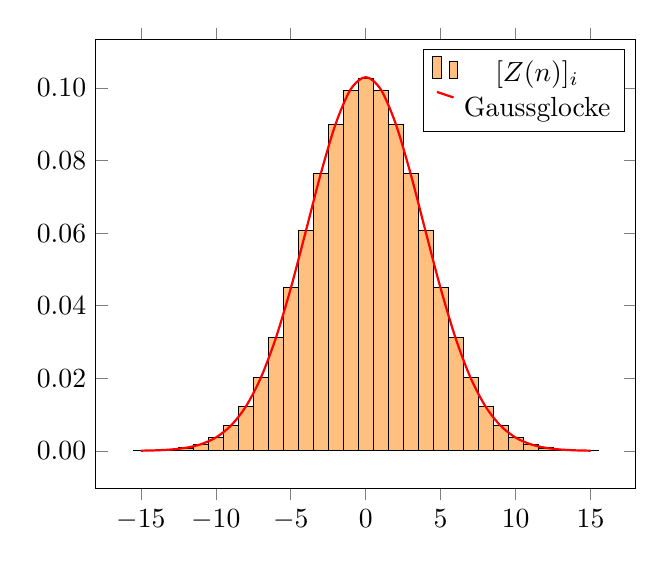
\begin{tikzpicture}[
    declare function={binom(\k,\n,\p)=\n!/(\k!*(\n-\k)!)*\p^\k*(1-\p)^(\n-\k);}
]
\begin{axis}[
    samples at={-15,...,15},
    yticklabel style={
        /pgf/number format/fixed,
        /pgf/number format/fixed zerofill,
        /pgf/number format/precision=2
    },
    ybar=0pt, bar width=1
]
\addplot [fill=orange, fill opacity=0.5] {binom(x+30,60,0.5)}; \addlegendentry{$[Z(n)]_i$}
    \addplot[draw=red,thick,smooth] {1/(sqrt(30*pi)) *exp(-1/30*x^2)}; \addlegendentry{\text{Gaussglocke}}
\end{axis}
\end{tikzpicture}
\caption{Binomialverteilung und Gaussglocke}
\end{figure}
Für $n\gg 1$ sieht diese Verteilung dann ungefähr wie die Gaussglocke aus. \\
\end{enumerate}
\underline{Skalierung:} Wir setzen nun
\[
    B(t) = \lim_{n \to \infty} \frac{Z(\left\lfloor nt \right\rfloor )}{\sqrt{n} }
.\] 
und dies ist dann die Brownsche Bewegung.

Nun möchten wir Vorhersagen treffen können:
\begin{question}
        Ist $Z(n)$ in einer gegebenen Menge  $A$?
\end{question}
Das kann man (im Allgemeinen) nicht einfach mit 'Ja' oder 'Nein' beantworten. Stattdessen müssen wir fragen:
\begin{question}
Wenn man $Z(n)$ beobachtet, wie häufig wird  $Z(n)$ in  $A$ sein?
\end{question}
Diese Frage lässt sich mit einer Zahl $\in [0,1]$ beantworten.

\subsection{Ereignisse und Wahrscheinlichkeiten}
Wir benötigen 3 Grundelemente:
\begin{enumerate}[(1)]
    \item Die Menge $\Omega$ von möglichen \vocab{Ergebnissen}. die Elemente von $\Omega$ heißen auch  \vocab{Elementarereignisse}.
    \item Die Menge $\mathcal{F}$ der \vocab{Ereignisse}. Ein Ereignis  $E$ ist eine Eigenschaft, die mit einer Teilmenge $G\subset \Omega$ assoziiert ist: $ω\in G \iff $ Eigenschaft $E$ ist erfüllt.
    \item Eine \vocab{Wahrscheinlichkeitsverteilung (auch W-maß)}:
        \[
            \mathbb{P}: \mathcal{F} \to  [0,1]
        .\] 
\end{enumerate}
\begin{remark*}
    Wir werden noch sehen, dass gewisse Dinge für unsere Begriffe erfüllt sein müssen, dazu aber später mehr.
\end{remark*}

\begin{example}
    Eine Urne hat 12 nummerierte Kugeln (von 1 bis 12).
    \begin{enumerate}[(1)]
        \item Das \vocab{Zufallsexperiment} besteht daraus, dass wir eine Kugel aus der Urne ziehen und die Zahl notieren, die wir sehen. D.h.
            \[
            \Omega = \left \{1,\ldots,12\right\} 
            .\] 
            Ein Elementarereignis ist nun z.B. gegeben durch $ω = \left \{5\right\}  \equiv 5$ (wir vereinfachen die Notation).
        \item Mögliche Ereignisse sind z.B:
            \begin{equation}
                \begin{split}
                    A &= \text{'Die Zahl ist gerade'} \\
                    B&= \text{'Die Zahl ist }\leq 5 \text{'}\\
                    C &= \text{'Die Zahl ist 8'}
                \end{split}
            \end{equation}
            Die assoziierten Mengen sind dann
            \begin{equation}
                \begin{split}
                    A &= \left \{2,4,6,8,10,12\right\}  \\
                     B &= \left \{1,2,3,4,5\right\} \\
                      C & = \left \{8\right\} 
                \end{split}
            \end{equation}
        \item Für die Wahrscheinlichkeiten nehmen wir an, dass jede Kugel die gleiche Chance hat, gezogen zu werden, d.h.
            \[
                \forall G\in \mathcal{F}: \mathbb{P}(G) = \frac{\abs{G}}{\abs{\Omega} }
            .\] 
            Wir erhalten nun die Wahrscheinlichkeiten
            \[
                \mathbb{P}(A) = \frac{6}{12}=\frac{1}{2} \qquad \mathbb{P}(B) = \frac{5}{12} \qquad \mathbb{P}(C) = \frac{1}{12}
            .\] 
    \end{enumerate}
\end{example}

\begin{notation}
    $A\equiv \left \{ω\in \Omega \mid  ω\in A\right\} \equiv  \left \{ω\in A\right\} \equiv \left \{A \text{ tritt ein}\right\} $
\end{notation}







    \lecture[$σ$-Algebren, Messräume. Wahrscheinlichkeitsverteilungen, Wahrscheinlichkeitsräume. Einschluss-Ausschluss-Prinzip. Endliche (diskrete) Wahrscheinlichkeitsräume.]{Mi 14 Apr 2021 10:17}{}
Wir kennen nun die Grundbegriffe $\Omega, \mathcal{F}, \mathbb{P}$ zur Beschreibung von Zufallsexperimenten, die wir uns nun genauer ansehen wollen:
\begin{question}
    Welche Struktur muss $\mathcal{F}$ besitzen.
\end{question}
Sein $A,B\in \mathcal{F}$, dann können wir das Ereignis $A \cap B$ betrachten, d.h. beide der Eigeschaften treten ein. Genauso sollte
 \[
A^{c} := \Omega \setminus A 
.\] 
, das \vocab{Komplement von $A$}, bzw. das \vocab{Gegenereignis} von $A$ ebenfalls in  $\mathcal{F}$  sein. Aus den beiden vorherigen Eigenschaften folgt bereits, dass
\[
    A \cup B= (A^{c} \cap B^{c})^{c}
.\] 
ebenfalls in $\mathcal{F}$ sein wird. \\
Eine Menge $\mathcal{F}$ mit solchen Eigenschaften heißt \vocab{Algebra}.
\begin{dnotation}
Seien nun $A,B$ und $(A_i)_{i\in I}$  Ereignisse, wobei $I$ endlich oder abzählbar sei. Dann notieren wir die folgenden Ereignisse:
\begin{enumerate}[label=\protect\circled{\alph*}]
    \item \emphasize{$A \cup B$} : $ω\in A \cup B \iff  ω\in A \lor ω\in B$, d.h. $A\cup B$ tritt ein, genau dann, wenn  $A$ eintritt oder  $B$ eintritt.
        \item  \emphasize{$\bigcup_{i \in  I} A_i$}: $ω\in \bigcup_{i \in  I} A_i$, wenn es ein $i\in I$ gibt, sodass $\omega \in A_i$
    \item  \emphasize{$A \cap B$}: $\omega\in A \cap B \iff  $ A \underline{und} B treten ein.
        \item \emphasize{$\bigcap_{i \in I} A_i$}: $\omega\in \bigcap_{i \in I}A_i \iff \forall i \in I \colon$ $A_i$ tritt ein.
            \item \emphasize{$A = \emptyset$} ist das Ereignis, das  \underline{nie} eintritt. \\
                \emphasize{$A = \Omega$} ist das Ereignis, dass \underline{immer} eintritt.
\end{enumerate}
\end{dnotation}

\begin{definition}[$\sigma$-Algebra]\label{def:sigma-algebra}
    Eine  \vocab{$\sigma$-Algebra} ist eine nicht leere Menge $\mathcal{F}$ von Teilmengen von $\Omega$ mit den Eigenschaften:
    \begin{enumerate}[label=\protect\circled{\alph*}]
        \item $\Omega \in \mathcal{F}$
        \item $\forall A\in \mathcal{F} \colon A^{c}\in \mathcal{F}$.
        \item Falls $(A_i)_{i \in I}\in \mathcal{F}$, dann auch $\bigcup_{i=1} ^{\infty}A_i \in \mathcal{F}$
    \end{enumerate}
    Wir nennen $(\Omega,\mathcal{F})$ dann einen \vocab{Messraum}. 
\end{definition}

\begin{lemma}\label{lm:weitere-eigenschaften-einer-sigma-algebra}
    Sei $\mathcal{F}$ eine $\sigma$-Algebra, dann ist:
    \begin{enumerate}[label=\protect\circled{\alph*}]
        \item $\emptyset\in \mathcal{F}$
        \item $A,B \in \mathcal{F} \implies A \cup B \in \mathcal{F}$ und $A\cap B \in \mathcal{F}$.
        \item $(A_i)_{i \in I}\in \mathcal{F} \implies \bigcap_{i=1}^{\infty}A_i \in \mathcal{F}$.
    \end{enumerate}
\end{lemma}
\begin{proof}
    \begin{enumerate}[label=\protect\circled{\alph*}]
        \item $\emptyset = \Omega^{c} \in \mathcal{F}$ nach Eigenschaften \circled{a} und \circled{b} aus der Definition.
        \item $A \cup B = A \cup B \cup \emptyset \cup \emptyset \ldots \in \mathcal{F}$ nach Eigenschaften  \circled{b} und \circled{c}. $A \cap B = (A^{c}\cup B ^{c})^{c} \in \mathcal{F}$
        \item $\bigcap_{i=1}^{\infty}A_i = \left( \bigcup_{i=1}^{\infty}A_i^{c} \right) ^{c}\in \mathcal{F}$ nach \circled{b} und \circled{c}.
    \end{enumerate}
\end{proof}

Wir haben nun $(\Omega, \mathcal{F})$ näher untersucht, es fehlt nun noch $\mathbb{P}$. 
\begin{question}
    Welche Eigenschaften soll $\mathbb{P}$ (das Wahrscheinlichkeitsmaß bzw. die Wahrscheinlichkeitsverteilung) besitzen?
\end{question}
Seien $A,B \in \mathcal{F}$ mit $A\cap B = \emptyset$, d.h. $A$ und $B$ können nicht gleichzeitig eintreten. Dann fordern wir
\[
    \mathbb{P}(A \cap B) = \mathbb{P}(A) + \mathbb{P}(B) \quad \text{(endliche Additivität)}
.\] 
Dazu wollen wir, dass $\Omega \in \mathcal{F}$ immer eintritt, d.h. $\mathbb{P}(\Omega) = 1 \equiv  100\%$ (Normierung).

\begin{definition}[Wahrscheinlichkeitsverteilung]\label{def:wahrscheinlichkeitsverteilung}
Sei $(\Omega, \mathcal{F})$ ein Messraum. Eine Abbildung $\mathbb{P} : \mathcal{F} \to  \R_+$ ist eine \vocab{Wahrscheinlichkeitsverteilung} auf $(\Omega, \mathcal{F})$, falls
    \begin{enumerate}[(1)]
        \item $\mathbb{P}(\Omega) = 1$
        \item Sind $(A_i)_{i \in I}\in \mathcal{F}$ paarweise disjunkt, so ist:
            \[
                \mathbb{P}\left( \bigcup_{i=1}^{\infty}A_i \right) = \sum_{i=1}^{\infty} \mathbb{P}(A_i) \quad (\sigma\text{-Additivität})
            .\] 
    \end{enumerate}
\end{definition}
\begin{remark*}
    Die Definition macht implizit Gebrauch davon, dass die linke Seite überhaupt definiert ist. Dies folgt jedochdaraus, dass $\mathcal{F}$ eine $\sigma$-Algebra ist.
\end{remark*}

\begin{definition}[Wahrscheinlichkeitsraum]\label{def:wahrscheinlichkeitsraum}
    Ein \vocab{Wahrscheinlichkeitsraum $(\Omega, \mathcal{F},\mathbb{P})$} besteht aus einer Menge $\Omega$, einer  $\sigma$-Algebra $F\subset \mathbb{P}\mathcal{(\Omega)}$ und einem Wahrschenilichkeitsmass $\mathbb{P}$ auf $(\Omega, \mathcal{F})$ 
\end{definition}


\begin{lemma}\label{lm:weitere-eigenschaften-eines-wahrscheinlichkeitsraums}
    Sei $(\Omega, \mathcal{F}, \mathbb{P})$ ein Wahrscheinlichkeitsraum. Dann ist
\begin{enumerate}[label=\protect\circled{\alph*}]
    \item $\mathbb{P}(\emptyset)=0$ 
    \item $\forall A,B\in \mathcal{F}$ mit $A\cap B = \emptyset$ ist
        \[
            \mathbb{P}(A\cup B ) = \mathbb{P}(A) + \mathbb{P}(B)
        .\] 
    \item      $\forall A,B\in \mathcal{F}$ mit $A\subset B$ ist 
        \begin{equation*}
            \begin{split}
                \mathbb{P}(B) &= \mathbb{P}(A) + \mathbb{P}(B \setminus A)  \\
                \mathbb{P}(A^{c}) &= 1 - \mathbb{P}(A) \\
                \mathbb{P}(A) &\leq  \mathbb{P}(B) \leq  1
            \end{split}
        \end{equation*}
    \item $\forall A,B \in \mathcal{F}$ ist
        \begin{equation*}
            \begin{split}
                \mathbb{P}(A \cup B) &= \mathbb{P}(A) + \mathbb{P}(B) - \mathbb{P}(A\cap B) \\
                                     &\leq  \mathbb{P}(A) + \mathbb{P}(B)
            \end{split}
        \end{equation*}
    \item Wenn $A_n \nearrow A$ ,d.h. $A_1\subset A_2\subset \ldots$ mit $\bigcup_{i =1}^{\infty} A_i = A$ (monotone Konvergenz von Mengen), oder $A_n \searrow A$ (d.h.  $A_1\supset A_2 \supset \ldots$ mit $\bigcap_{i=1}^{\infty} A_i = A $ ), so ist
        \[
            \lim_{n \to \infty} \mathbb{P}(A_n) = \mathbb{P}\left( \lim_{n \to \infty} A_n \right)  = \mathbb{P}(A)
        .\] 
\end{enumerate}
\end{lemma}
\begin{proof}
    \begin{enumerate}[label=\protect\circled{\alph*}]
        \item Wir wissen:
            \[
                1= \mathbb{P}(\Omega) = \mathbb{P}\left( \Omega \cup \emptyset \cup \emptyset \cup \emptyset \ldots  \right)  = \mathbb{P}(\Omega) + \mathbb{P}(\emptyset) + \mathbb{P}(\emptyset) + \ldots
            .\] 
            subtrahieren von $\mathbb{P}(\Omega) =1$ liefert dann $\mathbb{P}(\emptyset) = 0$.
        \item Sei $A \cap B = \emptyset$, dann ist:
            \begin{equation*}
                \begin{split}
                    \mathbb{P}(A\cup B ) &= \mathbb{P}(A \cup B \cup \emptyset \cup \emptyset \cup \ldots) \\
                                         &\stackrel{σ-\text{Additivität}}{=} \mathbb{P}(A) + \mathbb{P}(B) + \mathbb{P}(\emptyset) + \mathbb{P}(\emptyset) + \ldots \\
                                         &= \mathbb{P}(A) + \mathbb{P}(B)
                \end{split}
            \end{equation*}
        \item Sei $A\subset B$. Dann ist $B = A \cup (B \setminus A)$ eine disjunkte Vereinigung, also erhalten wir
            \[
                \mathbb{P}(B) = \mathbb{P}(A) + \underbrace{\mathbb{P}(B \setminus A)}_{\geq 0} \geq  \mathbb{P}(A)
            .\] 
            Mit $B = \Omega$ ergibt sich  $1 = \mathbb{P}(A) + \mathbb{P}(A^{c})$
        \item Es ist
            \begin{equation}
                \begin{split}
                    \mathbb{P}(A \cup B) &= \mathbb{P}(A) + \mathbb{P}((A \cup B) \setminus A)  \\
                                         &= \mathbb{P}(A) + \mathbb{P}(B \setminus (A \cap B)) \\
                                         &= \mathbb{P}(A) + \mathbb{P}(B) - \underbrace{\mathbb{P}(A \cap B)}_{\geq 0} \\
                                         &\geq \mathbb{P}(A) + \mathbb{P}(B)
                \end{split}
            \end{equation}
        \item Übung
    \end{enumerate}
\end{proof}
\begin{corollary}[Einschluss-Ausschluss-Prinzip]\label{cor:einschluss-ausschluss-prinzip}
    Seien $A_1,\ldots,A_n \in \mathcal{F}$. Dann gilt
    \[
        \mathbb{P}(A_1 \cup \ldots \cup A_n) = \sum_{k=1}^{n} (-1)^{k-1} \sum_{1\leq i_1<i_2<\ldots<i_k \leq n} \mathbb{P}(A_{i_1} \cap A_{i_2} \cap \ldots \cap A_{i_k})
    .\] 
\end{corollary}
\begin{proof}
    Per Induktion, der Induktionsanfang lautet  $\mathbb{P}(A_1) = \mathbb{P}(A_1)$ und ist offensichtlich wahr. \\
    Die Aussage gelte nun für ein $n\in \N$, dann erhalten wir
    \begin{equation}
        \begin{split}
            \mathbb{P}\left( \bigcup_{i=1}^{n+1} A_i \right)  &= \mathbb{P}\left( \left(\bigcup_{i=1}^{n}A_i \right) \cup A_{n+1}\right)  \\
                                                              &= \mathbb{P}\left(\bigcup_{i=1}^{n} A_i\right) + \mathbb{P}(A_{n+1}) - \mathbb{P}\left( \left( \bigcup_{i=1}^n A_i \right) \cap A_{n+1} \right)  \\
                                                              &= \mathbb{P}\left( \bigcup_{i=1}^{n} A_i \right)  + \mathbb{P}(A_{n+1}) - \mathbb{P}\left( \bigcup_{i=1}^n \underbrace{(A_i \cap _{A_{n+1}})}_{=: \tilde{A}_i} \right)  \\
                                                              &= \sum_{k=1}^{n} (-1)^{k-1} \sum_{1\leq i<\ldots<i_k \leq n} \mathbb{P}(A_{i_1} \cap \ldots \cap A_{i_k}) + \mathbb{P}(A_{n+1}) \\
                                                              &\qquad -\sum_{k=1}^n (-1)^{k-1} \sum_{1\leq i_1 < \ldots < i_k \leq n} \mathbb{P}(\underbrace{\tilde{A}_{i_1} \cap \ldots \cap \tilde{A}_{i_k}}_{A_{i_1} \cap \ldots \cap A_{i_k} \cap A_{n+1}})
        \end{split}
    \end{equation}
    Andererseits ist aber auch:
    \begin{alignat*}{5}
           &\quad&  &\sum_{k=1} ^{n+1} (-1)^{k-1} \sum_{1\leq i_1<\ldots<i_k \leq  n+1} \mathbb{P}(A_{i_1} \cap \ldots \cap A_{i_k}) &\quad & \\
           &= & &\sum\limits_{k=1}^{n}(-1)^{k-1} \sum\limits_{1\leq i_1< \ldots < i_k \leq  \color{red} n} \mathbb{P}(A_{i_1} \cap \ldots \cap A_{i_k}) & \quad &\Big\}\text{\parbox{2cm}{Terme mit $i_k\leq n$}} \\
           &+& &\underbrace{\sum_{k=2}^{n+2} (-1)^{k-1} \sum_{1\leq i_1<\ldots<i_{k-1}\leq n} \mathbb{P}(A_i \cap \ldots \cap A_{i_{k-1}} \cap A_{n+1})}_{\stackrel{l := k-1}{=} -\sum\limits_{l=1}^n (-1)^{l-1}\sum\limits_{1\leq i_1<...<i_l\leq n} \mathbb{P}(A_{i_1} \cap \ldots \cap A_{i_l} \cap A_{n+1})}& \quad &\Bigg\}\text{\parbox{2cm}{\small Terme mit $i_k = n+1$ und  $k\geq 2$}}\\
           &+& & \mathbb{P}(A_{n+1}) \qquad& \quad  &\Big\}\text{\parbox{2cm}{\small Terme mit $i_k = n+1$ und  $k=1$}}
    \end{alignat*}
    und damit sehen wir, dass die beiden Ausdrücke übereinstimmen, also ist der Induktionsschritt erbracht.
\end{proof}


\subsection{Diskrete Verteilungen}
\begin{itemize}
    \item Sei nun $\Omega$ endlich oder abzählbar.
    \item Falls wir $\mathcal{F}$ nicht explizit angeben, dann wird $\mathcal{F} = \mathcal{P}(\Omega)$ gewählt, d.h.
        \[
            \operatorname{Card} (\mathcal{P}(\Omega)) \equiv \abs{\mathcal{P}(\Omega)} = 2 ^{ \abs{\Omega}} 
        .\] 
\end{itemize}
\begin{example}[Münzwurf]
    Es sei $\Omega = \left \{K,Z\right\}$, wobei $K$ für Kopf stehe und $Z$ für Zahl. Dann ist
    \[
    \mathcal{F} = \left \{\left \{K\right\} ,\left \{Z\right\} ,\left \{Z,K\right\} ,\emptyset\right\} 
    .\] 
    Sei $p\in [0,1]$ die Wahrscheinlichkeit, dass man Kopf erhält. Da $\mathbb{P}$ für alle Element aus $\mathcal{F}$ definiert sein muss, erhalten wir
    \[
        \mathbb{P}(\emptyset) = 0 \qquad \mathbb{P}(K) = p, \qquad \mathbb{P}(Z) = \mathbb{P}(K^{c}) = 1-p \qquad \mathbb{P}(\left \{Z,K\right\} ) = \mathbb{P}(\Omega) = 1
    .\] 
\end{example}
\begin{question}[Charakterisierung von diskreter Wahrscheinlichkeit]
Was müssen wir fordern, sodass $\mathbb{P}$ auf $\mathcal{P}(\Omega)$ gibt?.
\end{question}
\begin{example}
    $\Omega = \left \{1,2,\ldots,10\right\}$ würde genügen, da dann $\abs{\mathcal{P}(\Omega)}= 2^{\abs{\Omega} }=2^{10} = 1024 $
    endlich (diskret) ist.
\end{example}

    \lecture{3}{Di 20 Apr 2021 12:16}{Trennungsaxiome, Kompaktheit}
\begin{proof}
    Betrachte die stetige Abbildung
        \begin{equation*}
        f': \left| \begin{array}{c c l} 
            [0,1] & \longrightarrow & S^1\subset \C \\
        t & \longmapsto &  e^{2\pi it}
        \end{array} \right.
    \end{equation*}
    Wir sehen $f'(0) = f'(1) = 1$, also existiert nach der universellen Eigenschaft ein  $f$, sodass folgendes kommutiert: \\
     \begin{tikzcd}
         \left[ 0,1\right] \ar[two heads]{d}\ar{r}{f'} & S^1 \\
         \left[ 0,1 \right] / (0 \sim 1) \ar[swap,two heads]{ur}{f}
    \end{tikzcd}
    und $f$ stetig ist. Zudem ist  $f$ bijektiv. Es bleibt zu zeigen, dass  $f^{-1}$ stetig ist, das zeigen wir jedoch nicht jetzt (ginge mit viel rechnen), sondern später, wenn wir mehr Technik haben. Anschaulich ist das jedoch klar:
\begin{figure}[ht]
    \centering
    \incfig{intervall-und-kreis-sind-homeomorph}
    \caption{$[0,1] / (0\sim 1)$ und $S^1$ sind homöomorph}
    \label{fig:intervall-und-kreis-sind-homeomorph}
\end{figure}
\end{proof}
\begin{remark}
    Die Abbildung
        \begin{equation*}
        \begin{array}{c c l} 
            [0,1) & \longrightarrow & S^1 \\
        t & \longmapsto &  e^{2\pi it}
        \end{array}
    \end{equation*}
    ist stetig und bijektiv, allerdings kein Homöomorphismus, denn $\left[ 0, \frac{1}{2} \right] \subset [0,1)$ ist offen, aber $f(\left[ 0,\frac{1}{2} \right] ) = \left( f^{-1} \right) ^{-1}\left( \left[ 0,\frac{1}{2} \right]  \right) $ ist nicht offen im Kreis.
\end{remark}
\begin{example}
    \begin{itemize}
        \item Sei $X = [0,1]^2 \subset \R$. Identifiziere nun $(t,0) \sim  (t,1)$ sowie $(0,s) \sim  (1,s)$ für $s,t\in [9,1]$. Dann ist $X / \sim $ der Torus.
        \item Sei $X = [0,1] ^2 \subset \R^2$. Identifizieren wir $(t,0) \sim  (t,1)$ sowie $(0,s) \sim  (1, 1-s)$, so erhalten wir die \vocab{Kleinsche Flasche}. 
        \item Betrachte auf dem $\R^{n+1}\setminus \left \{0\right\} $ die Relation $x \sim  λx$ für $λ>0\in \R$. Dann ist $\R^{n+1} / \sim  \cong S^n$. Zunächst ist nämlich die Abbildung
                \begin{equation*}
                f: \left| \begin{array}{c c l} 
                \R^{n+1}\setminus \left \{0\right\}  & \longrightarrow & S^n \\
                x & \longmapsto &  \frac{x}{\lVert x \rVert _2}
                \end{array} \right.
            \end{equation*}
            stetig und die induzierte Abbildung $\R^{n+1} \setminus \left \{0\right\}  / \sim \to  S^n$ ist bijektiv. Das rechnen wir nach: Seien $x\neq y$ mit $d(x,y) < \delta$, so ist:
            \begin{equation}
                \begin{split}
                    d\left( \frac{x}{\lVert x \rVert },\frac{y}{\lVert y \rVert } \right) &\leq d\left( \frac{x}{\lVert x \rVert },\frac{y}{\lVert x \rVert } \right) + d\left( \frac{y}{\lVert x \rVert },\frac{y}{\lVert y \rVert } \right)  \\
                                                                                          &= \frac{1}{\lVert x \rVert } d(x,y) + \sqrt{\sum \left( \frac{y_i}{\lVert x \rVert }-\frac{y_i}{\lVert y \rVert } \right)^2 }  \\
                                                                                          &= \frac{1}{\lVert x \rVert } d(x,y) + \sqrt{\frac{(\lVert x \rVert -\lVert y \rVert )^2}{\lVert x \rVert \lVert y \rVert }} \lVert y \rVert \\
                                                                                          &< \frac{1}{\lVert x \rVert }\cdot \delta + \frac{\delta}{\lVert x \rVert ^2 + \delta \lVert x \rVert }(\lVert x \rVert +\delta) \to  0
                \end{split}
            \end{equation}
            also ist $f$ stetig. Mit der Inklusion  $ι: S^n \to  \R^{n+1} \setminus \left \{0\right\} $ erhalten wir
            \[
            f \circ  ι = \id_{S^n}
            .\] 
            Übung: Daraus folgt bereits, dass $S^n$ die Quotiententopologie trägt.
        \item Setzen wir erneut $X = \R^{n+1} \setminus \left \{0\right\} $, aber diesmal $x \sim  \lambda x$ für $λ\in \R \setminus  \left \{0\right\} $, so heißt der Quotient
            \[
            X / \sim  =: \R P^n
            .\] 
            der \vocab[Raum!reell projektiv]{reelle projektive Raum}.  Es ist
            \[
                \R P^n \cong S^n / (x \sim -x)
            .\] 
            Dies sehen wir mittels folgendem Diagramm: \\
            \begin{tikzcd}
                \R^{n+1} \setminus \left \{0\right\}  \ar[two heads]{d} \ar[shift left]{r}{f} & S^n \ar[shift left]{l}{ι} \ar[two heads]{d} \\
                \R P^n \ar[dashed, shift left]{r}{\overline{f}} & S^n / (x \sim  - x) \ar[dashed, shift left]{l}{\overline{ι}}
            \end{tikzcd}
            \\
            Die Abbildungen $\overline{ι}$ und $\overline{f}$ sind stetig nach der universellen Eigenschaft und invers zueinander.
        \item Sei $X$ ein topologischer Raum und  $A\subset X$ eine Teilmenge. Definiere die Relation $\sim $ durch $a\sim a'$ für $a,a'\in A$ (bzw. erzeuge eine dadurch). Dann setzen wir
            \[
            X / A := X / \sim 
            .\] 
            Es ergibt sich
            \begin{itemize}
                \item $[0,1] / \left \{0,1\right\} \cong S^1$ 
                \item $[0,1] / [0,1)$ hat zwei Punkte  $[0,1)$ und  $\left \{1\right\} $. Es ist $[0,1) \subset [0,1]$ offen, aber $\left \{1\right\} $ nicht, also handelt es sich um den Sierpinski-Raum.
            \end{itemize}
    \end{itemize}
\end{example}
\begin{remark}
    Quotientenräume von metrischen Räumen sind im Allgemeinen nicht metrisierbar.
\end{remark}

\section{Trennungsaxiome}
\begin{definition}[Hausdorff'sch]\label{def:hausdorff}
    Ein topologischer Raum heißt \vocab{Hausdorff} (oder \vocab[Hausdorff!Hausdorffsch]{Hausdorffsch}), wenn $\forall x,y\in X$ mit $x\neq y$ offene Mengen $U_x, U_y\subset X$ existieren mit $x\in U_x$ und $y\in U_y$, sodass $U_x \cap U_y = \emptyset$. Diese Eigenschaft heißt auch Trennungsaxiom\index{Trennungsaxiom} \vocab[Trennungsaxiom!$T_2$]{$T_2$}. \\
    \begin{minipage}{\textwidth}
    \centering    
\begin{minipage}{0.3\textwidth}
        \centering
        \incfig{hausdroff-raum}
    \end{minipage}
    \end{minipage}
\end{definition}

\begin{theorem}\label{thm:metrisierbarer-raum-ist-hausdorff}
    Ist $X$ metrisierbar, so ist  $X$ Hausdorffsch.
\end{theorem}
\begin{proof}
    Sei $d$ eine Metrik auf  $X$, die die Topologie induziert. Seien  $x,y\in X$ mit $x\neq y$. Setze
    \[
        U_x := U\left( x, \frac{d(x,y)}{2} \right) \qquad U_y = U\left( y, \frac{d(x,y)}{2} \right) 
    .\] 
    Dann ist $U_x \cap U_y = \emptyset$, denn für alle $z\in U_x \cap U_y$ ist
    \[
        d(x,y) \leq  d(x,z) + d(z,y) < \frac{d(x,y)}{2} + \frac{d(x,y)}{2} = d(x,y)
    .\] 
    , was nicht sein kann.
\end{proof}
\begin{example}
    $\R^n$ ist Hausdorffsch.
\end{example}
\begin{theorem}\label{thm:hausdorff-impliziert-t1}
    Ist $X$ Hausdorffsch und  $x\in X$, dann ist $\left \{x\right\} \subset X$ abgeschlossen.
    \label{thm:point-in-hausdorff-space-is-closed}
\end{theorem}
\begin{proof}
    Für $y\neq x$ existiert $U_y$ offen mit  $x\not\in U_y$ und $y\in U_y$. Dann ist
    \[
    X \setminus \left \{x\right\}  = \bigcup_{y\neq x} U_y 
    .\] 
    offen.
\end{proof}
\begin{remark}
    Ein topologischer Raum, für den alle $\left \{x\right\} $ abgeschlossen sind, heißt \vocab[Trennungsaxiom!$T_1$]{$T_1$-Raum}.
\end{remark}

\begin{lemma}\label{lm:teilraum-von-hausdorffraum-ist-hausdorff}
    Sei $X$ Hausdorffsch und $A\subset X$ ein Teilraum. Dann ist auch $A$ Hausdorffsch.
\end{lemma}
\begin{proof}
    Sei $x\neq y\in A$. Dann existieren $U_x, U_y\subset X$ offen mit $x\in U_x$ und $y\in U_y$ sowie $U_x \cap U_y = \emptyset$. Dann sind
    \[
    U_x \cap A \qquad U_y \cap A \subset A
    .\] 
    offen in $A$ und erfüllen die Bedingungen.
\end{proof}


\begin{remark}
    Jeder diskrete Raum ist Hausdorffsch. Ist $X$ endlich und Hausdorffsch, so ist  $X$ diskret.
\end{remark}
\begin{proof}
    Für jedes $y\neq x$ existiert ein $U_x^y$ offen mit  $x\in U_x^y$ und $y\not\in U_x^y$. Dann ist aber
    \[
    \left \{x\right\}  = \bigcap_{y\neq x} U_x^{y}
    .\] 
    offen (da $X$ endlich), also ist $X$ diskret. Die Umkehrung ist offensichtlich.
\end{proof}
\begin{example}
    $S^n \subset \R^{n+1}$ ist Hausdorffsch.
\end{example}

\begin{definition}[Normal]\label{def:normal}
    Ein topologischer Raum heißt \vocab[Topologischer Raum!normal]{normal}, falls
    \begin{itemize}
        \item $X$ ist Hausdorffsch
        \item  $\forall A,B\subset X$ abgeschlossen mit $A \cap B = \emptyset$ existieren $U_A, U_B \subset X$ offen mit $A\subset U_A$, $B\subset U_B$ und $U_A \cap U_B = \emptyset$. Diese Eigenschaft heißt auch Trennungsaxiom \vocab[Trennungsaxiom!$T_4$]{$T_4$}. \\
            \begin{minipage}{\textwidth}
                \centering
                \begin{minipage}{0.3\textwidth}
    \incfig{normaler-raum}
                \end{minipage}
            \end{minipage}
    \end{itemize}
\end{definition}


\begin{remark}
    Manchmal gibt es diese Definition auch ohne Hausdorff'sch.
\end{remark}

\begin{theorem}\label{thm:metrischer-raum-ist-normal}
    Ist $X$ metrisierbar, dann ist  $X$ normal.
\end{theorem}

\begin{proof}
    Übung.
\end{proof}

\begin{definition}[Regulär]\label{def:regulär}
    Ein topologischer Raum $X$ heißt  \vocab[Topologischer Raum!regulär]{regulär}, falls $X$ Hausdorff ist und  $\forall  A \subset X$ abgeschlossen und $x\in X \setminus A$ existieren $U_a, U_{x}$ offen mit $A\subset U_A, x\in U_x$ und $U_A \cap U_x = \emptyset$. (Auch Trennungsaxiom \vocab[Trennungsaxiom!$T_3$]{$T_3$} genannt).
\end{definition}

Klar: $T_4 \implies T_3$


\section{Kompaktheit}
Aus der Analysis ist (vielleicht) folgender Satz bekannt.
\begin{theorem}[Heine-Borel]\label{thm:heine-borel}
    Für $X\subset \R^n$ sind äquivalent:
    \begin{enumerate}[1)]
        \item $X$ ist abgeschlossen und beschränkt.
        \item Jede offene Überdeckung von $X$ hat eine endliche Teilüberdeckung
    \end{enumerate}
\end{theorem}

\begin{recap}
    'Jede offene Überdeckung besitzt eine endliche Teilüberdeckung' bedeutet: \\
    Für jede Familie $\left \{U_i\right\} _{i \in I}$ mit $U_i \subset X$ offen und $X \subset \bigcup_{i \in I}U_i$ existiert eine endliche Teilmenge $J\subset I$ mit $X \subset \bigcup_{j\in J} U_j$
\end{recap}
\begin{proof}
    später.
\end{proof}

\begin{definition}[Kompaktheit]\label{def:kompakt}
    Ein topologischer Raum $X$ heißt  \vocab[Topologischer Raum!kompakt]{kompakt}, falls jede offene Überdeckung eine endliche Teilüberdeckung besitzt.
\end{definition}
\begin{remark}
    Manchmal heißt obige Definition auch quasi-kompakt, und kompakt bedeutet dann quasi-kompakt + Hausdorff.
\end{remark}

\begin{example}
   Die Räume
   \[
       [0,1] \subset \R \qquad S^n \subset \R^{n+1}
   .\] 
   sind beide kompakt (nach \ref{thm:heine-borel})
\end{example}

    \lecture{4}{Do 22 Apr 2021 10:15}{Mehr zu Kompaktheit, Hausdorffräumen und Homöomorphismen}
\begin{example}
    Zur Frage von letzter Woche (wenn wir einen Hausdorff-Raum haben und eine Äquivalenzrelation, deren Klassen abgeschlossen sind, ist dann der Quotient wieder  Hausdorff?): Wähle auf $[0,1]$ die Relation erzeugt von
     \[
    \frac{1}{n} \sim  1 - \frac{1}{n}
    .\] 
    für alle $n\in \N_>0$. Betrachte dann die Abbildung: 
    \[
        [0,1] \twoheadrightarrow [0,1] / \sim 
    .\] 
    Punkturbilder sind endlich, also abgeschlossen. Aber der Raum $[0,1] / \sim $ ist nicht hausdorffsch, denn wri können die Punkte $0,1$ nicht trennen.
\end{example}
\begin{theorem}\label{thm:abgeschlossene-menge-in-kompaktem-raum-ist-kompakt}
    Sei $X$ ein kompakter Raum und  $Y\subset X$ abgeschlossen. Dann ist $Y$ kompakt.
\end{theorem}
\begin{proof}
    Sei $\left \{U_i\right\} _{i \in I}$ eine offene Überdeckung von $Y$. Dann existieren $U_i' \subset X$ offen mit $U_i = U_i' \cap Y$. Die Familie
     \[
    \left \{U_i'\right\} _{i \in I}\cup \left \{\underbrace{X \setminus Y}_{\text{offen}}\right\} 
    .\] 
    ist nun eine offene Überdeckung von $X$. Dann existiert $J\subset I$ endlich, so dass
    \[
    \left \{U_j'\right\} _{j\in J} \cup \left \{X \setminus Y\right\} 
    .\] 
    die Menge $X$ überdeckt. Also ist  
    \[
        \left \{\underbrace{U_j' \cap Y}_{U_j}\right\} _{j\in J} \cup \left \{\underbrace{X \setminus Y \cap Y}_{=\emptyset}\right\}  
    \]
    eine endliche Überdeckung für $Y$.
\end{proof}
\begin{theorem}\label{thm:kompakte-menge-in-hausdorff-raum-ist-abgeschlossen}
    Sei $X$ ein Hausdorff-Raum und  $Y\subset X$ kompakt. Dann ist $Y$ abgeschlossen.
\end{theorem}

\begin{corollary*}\label{cor:abgeschlossen-gdw-kompakt-in-kompaktem-hausdorff-raum}
    Ist $X$ kompakt und Hausdorffsch, dann sind äquivalent:
\begin{enumerate}[1)]
        \item $Y\subset X$ ist abgeschlossen
        \item $Y$ ist kompakt.
    \end{enumerate}
\end{corollary*}
\begin{proof}
    Unmittelbare Konsequenz aus \autoref{thm:abgeschlossene-menge-in-kompaktem-raum-ist-kompakt} und \autoref{thm:kompakte-menge-in-hausdorff-raum-ist-abgeschlossen}.
\end{proof}
\begin{lemma}\label{lm:in-hausdorff-raum-sind-kompakte-mengen-t3}
    Sei $X$ ein Hausdorff Raum und  $Y\subset X$ kompakt. Dann existiert $\forall x\in X\setminus Y$ offene Teilmengen $U_{x,Y}$ und $V_{x,Y}$ von $X$ so dass:  $x\in U_{x,Y}$ und $Y\subset V_{x,Y}$ und $U_{x,Y} \cap V_{x,Y} = \emptyset$.
\end{lemma}
\begin{proof}
    Sei $x\in X\setminus Y$. $\forall y\in Y$ existieren $U_{x,y}$ und $V_{x,y}$ offen mit $x\in U_{x,y}$ und $y\in V_{x,y}$, weil $X$ Hausdorffsch. \\
    Dann ist  $\left \{V_{x,y} \cap Y\right\} _{y\in Y}$ eine offene Überdeckung von $Y$. Also existiert endliche Teilüberdeckung (da  $Y$ kompakt) induziert durch Punkte  $y_1,\ldots,y_n$. Also:
    \[
    Y\subset \bigcup_{i=1}^n V_{x,y_i}
    .\] 
    Sei
    \[
    V_{x,Y} := \bigcup_{i=1}^n V_{x,y_i} \qquad U_{x,Y} := \bigcap_{i=1}^n U_{x,y_i} 
    .\] 
    Es ist auch $x\in U_{x,Y}$, weil $x\in U_{x,y_i}$ für jedes $i$. Wir müssen also noch Disjunktheit prüfen, es ist:
     \[
    U_{x,Y} \cap V_{x,y_i} \subset U_{x,y_i} \cap V_{x,y_i} = \emptyset
    .\] 
    Also auch
    \[
        \emptyset=    U_{x,Y} \cap \bigcup_{i=1}^n V_{x,y_i} = U_{x,Y} \cap V_{x,Y}
    .\]
\end{proof}
    \begin{figure}[H]
    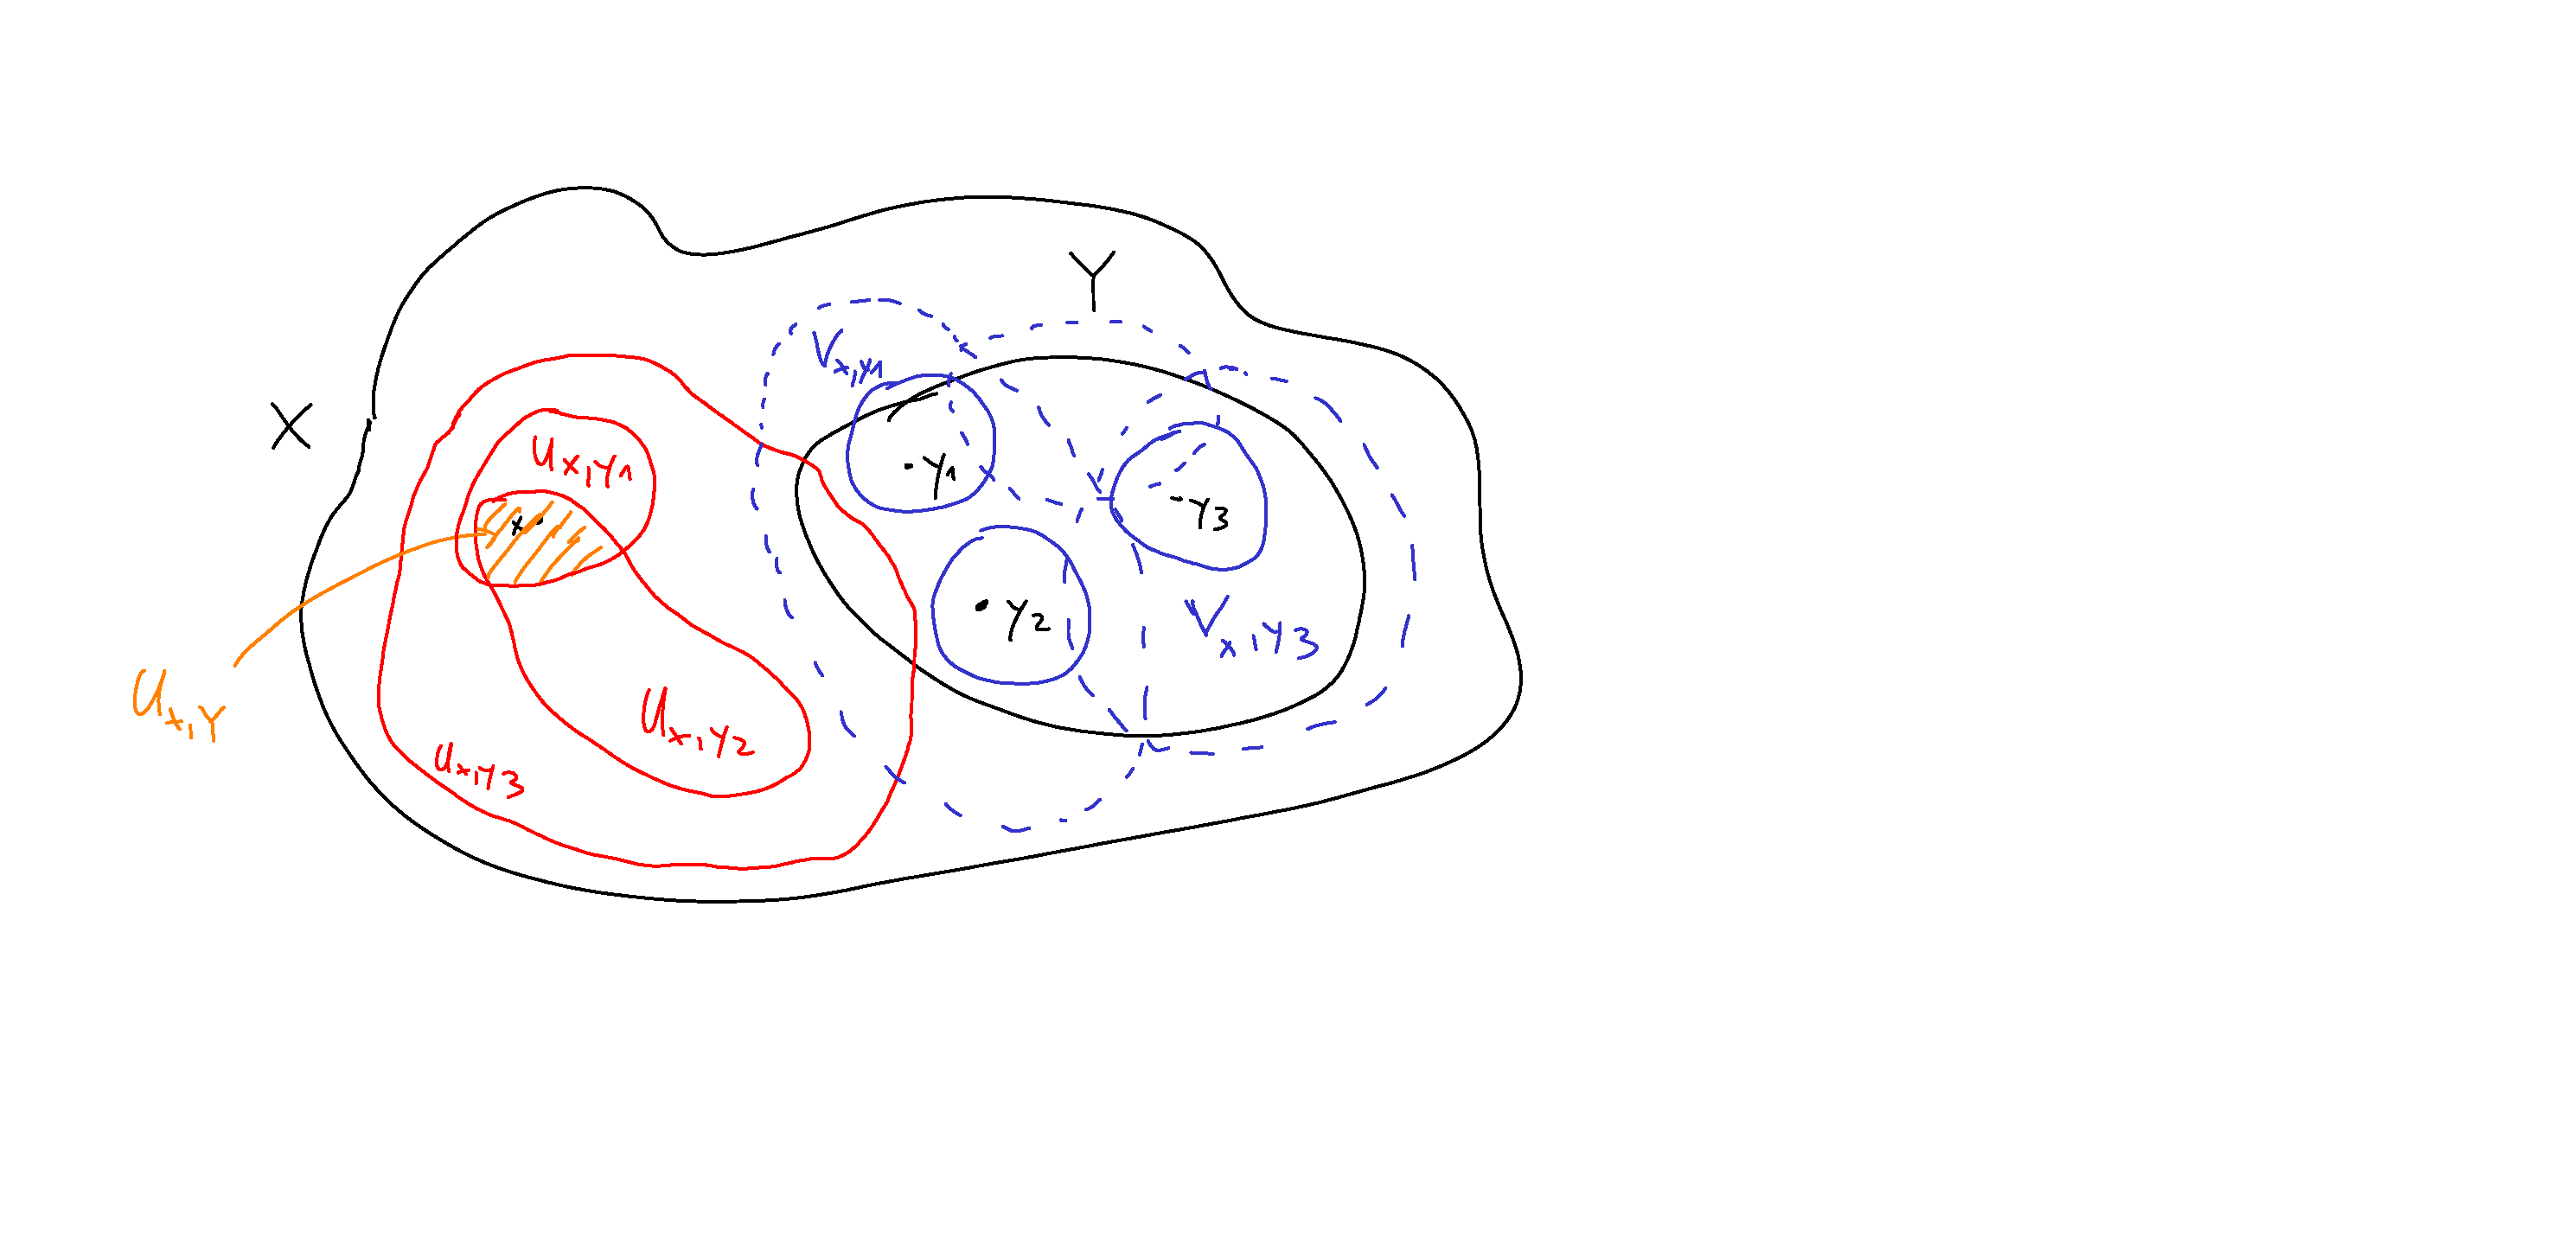
\includegraphics[scale=0.4]{figures/Lemma5.5.pdf}
    \caption{Skizze zum Beweis von Lemma \ref{lm:in-hausdorff-raum-sind-kompakte-mengen-t3}}
\end{figure}
\begin{proof}[Beweis von \autoref{thm:kompakte-menge-in-hausdorff-raum-ist-abgeschlossen}]
    Nach \autoref{lm:in-hausdorff-raum-sind-kompakte-mengen-t3} existieren $\forall x\in X \setminus Y$ ein $U_{x,Y}$ mit $x\in U_{x,Y}$ und $U_{x,Y} \cap Y = \emptyset$. Also ist
    \[
    X \setminus Y = \bigcup_{x\in X \setminus Y} U_{x,Y}
    .\] 
    offen und somit ist $Y$ abgeschlossen.
\end{proof}


\begin{example}['Gegenbeispiel' zu Satz \ref{thm:kompakte-menge-in-hausdorff-raum-ist-abgeschlossen}]
    Sei $G$ die Gerade mit zwei Urpsrüngen: \\
    Betrachte  $\R\cup \left \{0'\right\} $ mit $U$ Umgebung von  $a\in \R$ falls $\exists ε>0$ mit $(a-ε, a+ε)\subset U$ und $U$ Umgebung von  $0'$ und  $U$ Umgebung von  $0'$, falls  $\exists ε>0$ mit $(-ε,0 \cup (0,ε) \subset U$ und $0' \in U$. \\
    Wir können uns gewissermaßen  $0,0'$ gleichberechtigt vorstellen, nur dass die beiden Punkte verschieden sind. \\
    Dann ist  $[-1,1] \subset G$ kompakt (Übung!), aber nicht abegschlossen, da $0' \in G \setminus [-1,1]$ ist, dies aber keine Umgebung von $0'$ ist.
    \begin{figure}[H]
        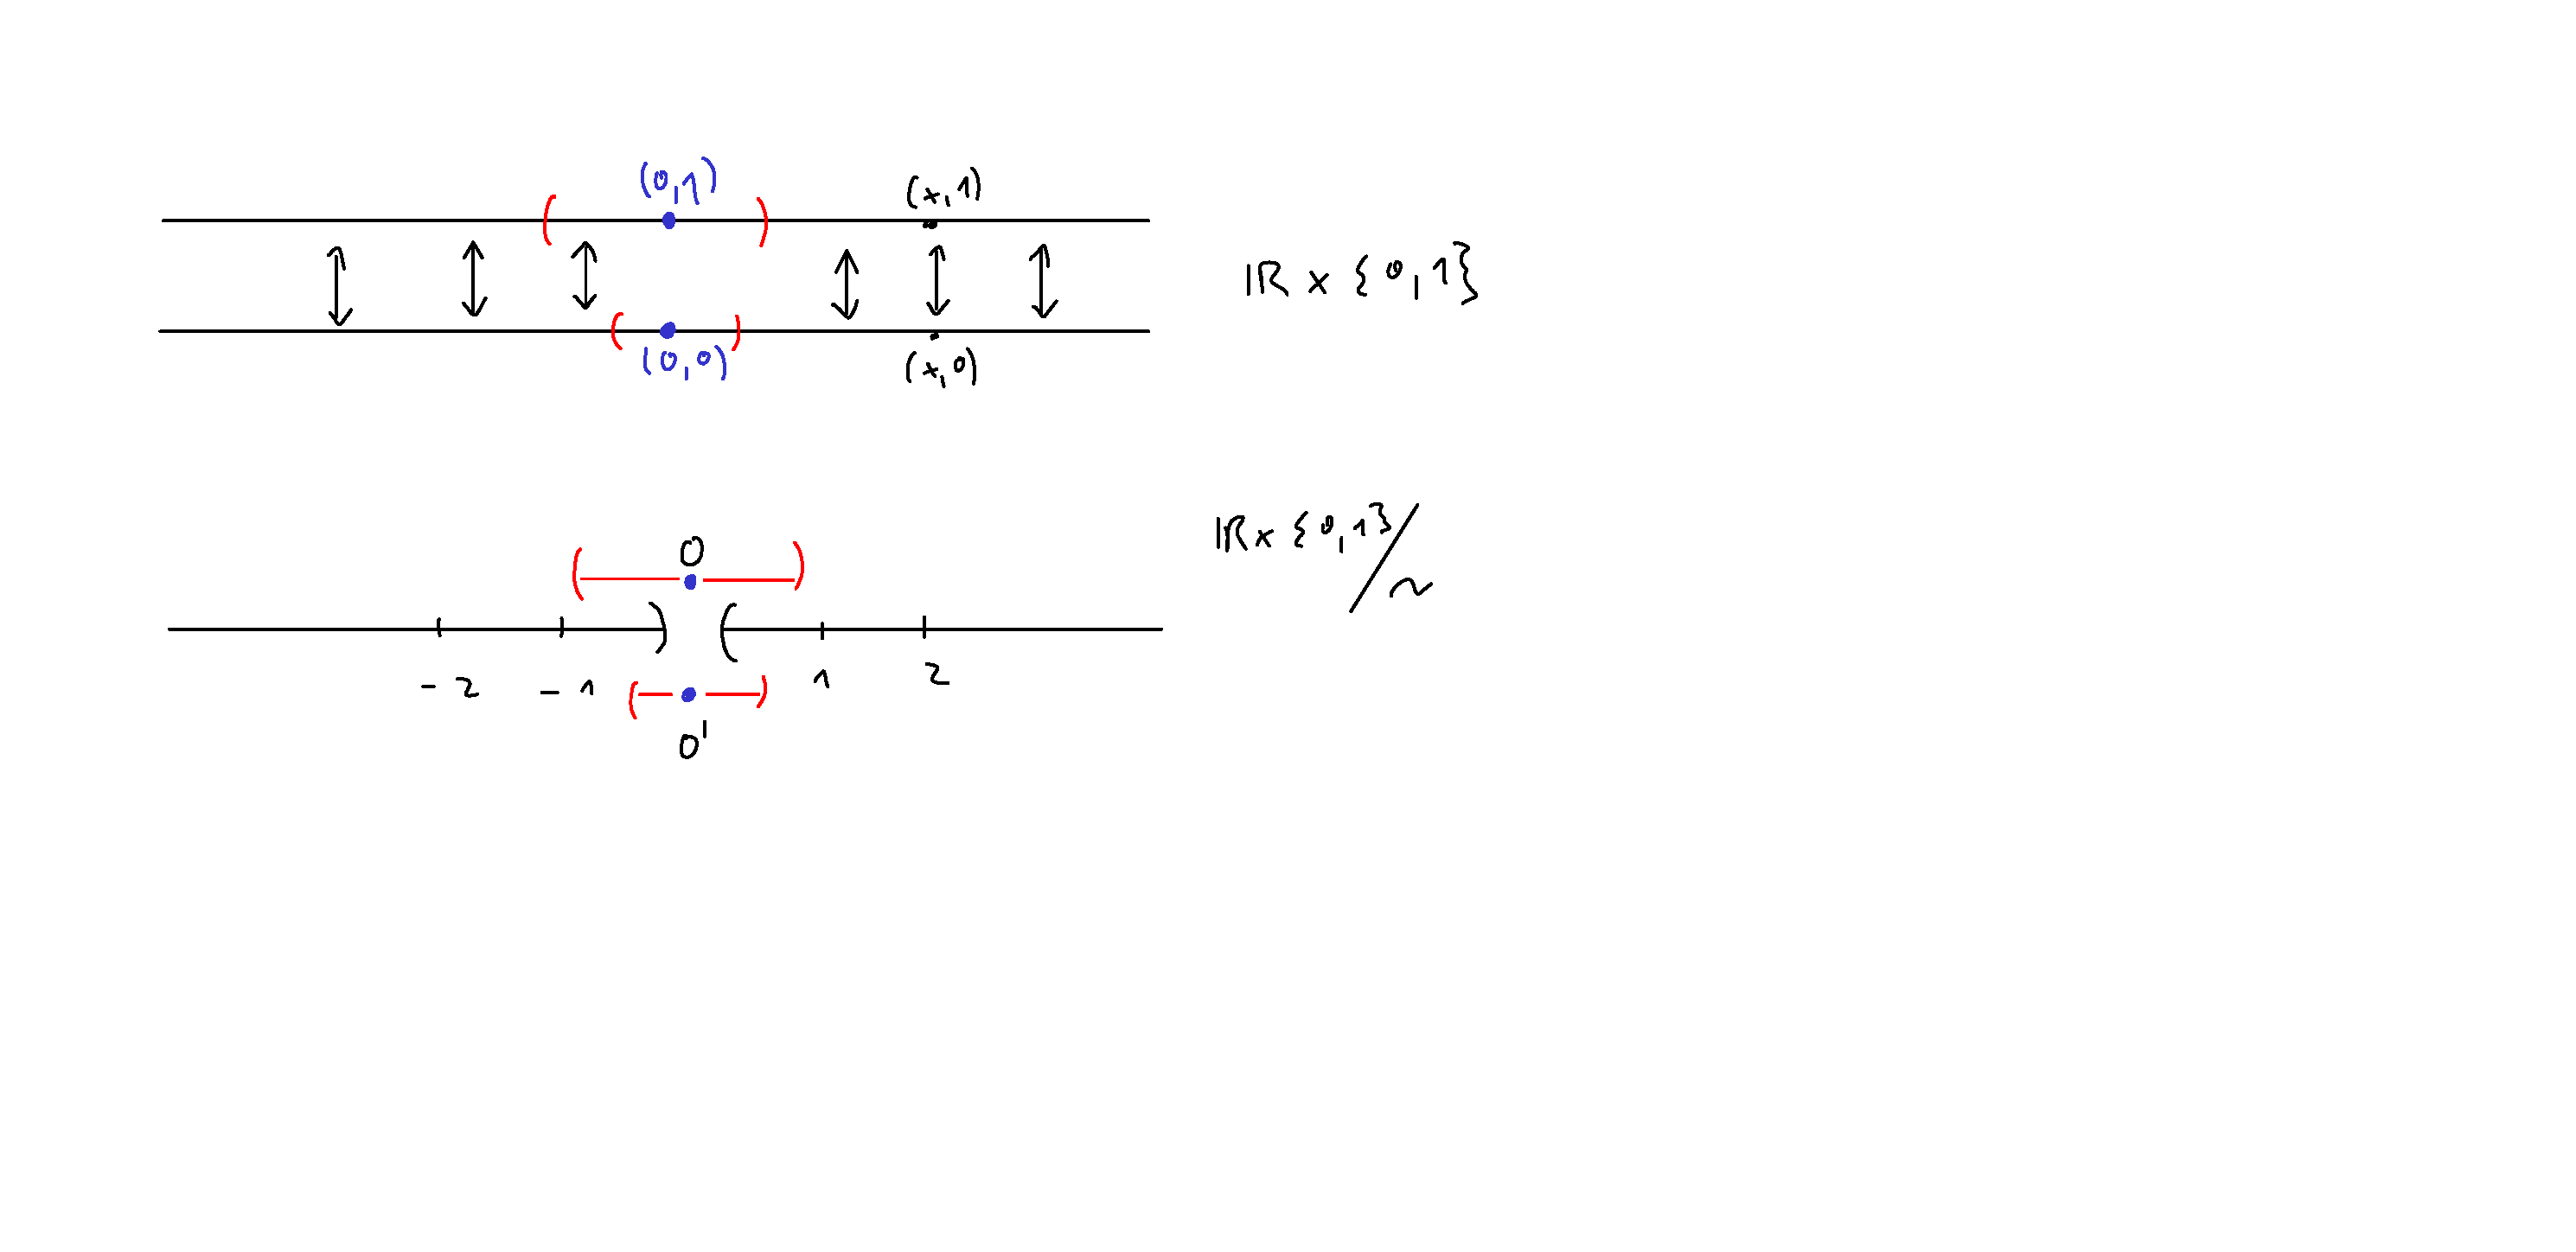
\includegraphics[scale=0.4]{figures/line-with-2-origins.pdf}
    \caption{Gerade mit 2 Ursprüngen}
    \end{figure}
\end{example}

Nun sind wir gewappnet für den
\begin{proof}[Beweis von \autoref{thm:heine-borel} (\nameref{thm:heine-borel})]
    '$2) \implies 1)$'. Sei $X\subset \R^n$ kompakt. Dann ist sie abgeschlossen nach \ref{thm:kompakte-menge-in-hausdorff-raum-ist-abgeschlossen}.
    Zudem ist $X\subset \bigcup_{x\in X} U(x,1)$ eine offene Überdeckung. Da $X$ kompakt finden wir endlich viele  $x_1,\ldots,x_n\in X$ mit
    \[
        X \subset \bigcup_{i=1}^n U(x_i,1)
    .\] 
    Also ist
    \[
        \diam(X) \leq  \max \left \{d(x_i,x_j)\right\} +2 < \infty
    .\] 
    und somit ist $X$ auch beschränkt. \\
    ' $1)\implies 2)$'. Da $X$ beschränkt ist,  $\exists m>0$ mit $X\subset [-m,m]^n\subset \R^n$. Da $X$ abgeschlossen ist, genügt es nach \autoref{thm:abgeschlossene-menge-in-kompaktem-raum-ist-kompakt} zu zeigen, dass  $[-m,m]^n$ kompakt ist. \\
    Wir führen einen Widerspruchsbeweis, nimm also an, dass  $[-m,m]^n$ nicht kompakt ist. Dann existiert eine offene Überdeckung  $\left \{U_i\right\} _{i \in I}$ ohne endliche Teilüberdeckung. \\
    \noindent\begin{minipage}{0.5\textwidth}
    Unterteile $[-m,m]^n$ in  $2^n$ gleich große Unterwürfel (halbiere jede Seite). Mindestens ein Unterwürfel hat keine endliche Teilüberdeckung. Unterteile diesen Würfel weiter und wähle wieder einen Unterwüfel, der keine endliche Teilüberdeckung hat. \\
    Wir erhalten eine Folge von Würfeln
     \[
         [-m,m]^n =     Q_0 \supset Q_1 \supset Q_2 \supset Q_3 \supset \ldots
    .\] 
    die jeweils keine endliche Teilüberdeckung durch $U_i's$ besitzen. \\
    \end{minipage}
    \begin{minipage}{0.5\textwidth}
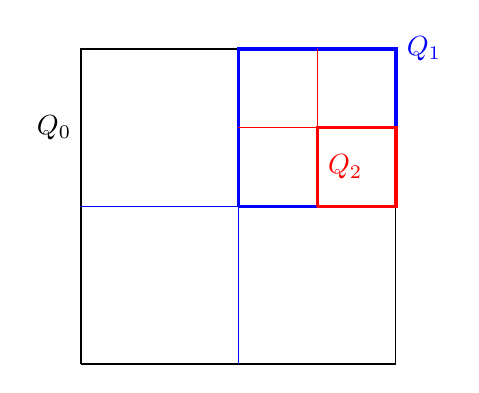
\begin{tikzpicture}
    \draw (-2,-2) -- (-2,2) node[near end, anchor=east]{$Q_0$}-- (2,2) -- (2,-2) -- (-2,-2);
    \draw[blue] (-2,0) -- (2,0);
    \draw[blue] (0,-2) -- (0,2);
    \draw[blue,very thick] (0,0) -- (2,0) -- (2,2) node[anchor=west]{$Q_1$} -- (0,2) -- (0,0) ; 
    \draw[red] (1,0) -- (1,2);
    \draw[red] (0,1) -- (2,1);
    \draw[red, very thick] (1,0) -- (1,1) node[anchor=west, midway]{$Q_2$} -- (2,1) -- (2,0) -- (1,0);
\end{tikzpicture}
    \end{minipage}
    Sei  $x_i \in Q_i$ beliebig. Dann ist $x_i$ eine Cauchy-Folge, also existiert $x = \lim_{i\to \infty} x_i$, und $x\in Q_0$, da $Q_0$ abgeschlossen. \\
    Somit gibt es ein $U_j$ mit  $x\in U_j$, da die $\left \{U_i\right\} _{i \in I}$ eine Überedeckung von $Q_0$ waren. Damit ist auch $U(x,ε) \subset U_j$ für ein $ε>0$. Wähle einen Würfel $x\in Q_k$ mit Kantenlänge $< \frac{ε}{\sqrt{n} }$, dann ist auch $Q_k \subset U(x,ε) \subset U_j$. Das ist aber ein Widerspruch dazu, dass $Q_k$ keine endliche Teilüberdeckung hat, \contra. \\
    Also ist  $Q_0$ kompakt.
\end{proof}



\begin{theorem}[Bilder kompakter Räume]\label{thm:bild-von-kompaktem-raum-ist-kompakt}
    Sei $f: X \to  Y$ stetig und surjektiv und $X$ kompakt. Dann ist auch  $Y$ kompakt. 
\end{theorem}
\begin{proof}
    Sei $\left \{U_i\right\} _{i \in I}$ offene Überdeckung von $Y$. Dann ist
     \[
         \left \{f^{-1}(U_i)\right\} _{i \in I}
    .\] 
    offene Überdeckung von $X$. Da  $X$ kompakt ist, gibt es  $J\subset I$ endlich mit $X = \bigcup_{j\in J} f^{-1}(U_j)$. Dann ist 
    \[
        Y = f(X) = \bigcup_{j\in J} f(f^{-1}(U_j)) = \bigcup_{j\in J} U_j
    .\] 
    Also existiert eine endliche Teilüberdeckung von $Y$.
\end{proof}
\begin{corollary}\label{cor:stetige-abbildung-von-kompaktem-raum-in-hausdorff-raum-ist-abgeschlossen}
    Sei $f: X \to  Y$ stetig, $X$ kompakt und  $Y$ Hausdorff. Dann ist  $f$ abgeschlossen, d.h. $\forall A\subset X$ abgeschlossen ist $f(A) \subset Y$ abgeschlossen.
\end{corollary}
\begin{proof}
    Sei $A\subset X$ abgeschlossen. Dann ist $A$ kompakt nach \autoref{thm:kompakte-menge-in-hausdorff-raum-ist-abgeschlossen}, also ist  $f(A)$ kompakt nach \autoref{thm:bild-von-kompaktem-raum-ist-kompakt} (weil $f: X \to f(A)\subset Y$ surjektiv ist). Damit ist dann $f(A)$ abegschlossen nach \autoref{thm:kompakte-menge-in-hausdorff-raum-ist-abgeschlossen}. \\
    Also sind Bilder abgeschlossener Mengen abgeschlossen.
\end{proof}

\begin{corollary}[Homöomorphismen]\label{cor:stetige-bijektion-von-kompaktem-raum-in-hausdorff-raum-ist-homöomorphismus}
    Ist $f: X \to  Y$ stetig und bijektiv, $X$ kompakt und  $Y$ Hausdorff, dann ist  $f$ ein Homöomorphismus.
\end{corollary}

\begin{proof}
    Wir müssen zeigen, dass die Umkehrabbildung stetig ist. Dafür reicht es zu zeigen, dass $\forall A\subset X$ abgeschlossen auch $f(A) = (f^{-1})^{-1}(A)$ abgeschlossen ist. Das gilt aber genau nach vorherigem \autoref{cor:stetige-abbildung-von-kompaktem-raum-in-hausdorff-raum-ist-abgeschlossen}
\end{proof}
\begin{corollary}\label{cor:abbildung-von-kompaktem-raum-in-hausdorff-raum-ist-quotientenabbildung}
    Sei $f: X \to  Y$ stetig und surjektiv, $X$ kompakt und  $Y$ Hausdorffsch. Dann trägt  $Y$ die Quotiententopologie, d.h.  $U\subset Y$ offen genau dann, wenn $f^{-1}(U) \subset X$ offen.
\end{corollary}

\begin{proof}
    '$\implies$' folgt wegen Stetigkeit. \\
    '$\impliedby$' Ist $f^{-1}(U) \subset X$ offen, dann ist $f^{-1}(Y \setminus U ) = X \setminus f^{-1}(U)$ abgeschlossen in $X$, also folgt aus dem \autoref{cor:stetige-abbildung-von-kompaktem-raum-in-hausdorff-raum-ist-abgeschlossen}
     \[
         Y \setminus U \stackrel{\text{surj.}}{=}   f\left( \underbrace{f^{-1}\left( Y \setminus U \right)}_{\text{abgeschlossen}}  \right) 
    .\] 
    abgeschlossen ist, also ist $U\subset Y$ offen.
\end{proof}
Kommen wir nun zum
\begin{proof}[Beweis von \autoref{thm:kreis-ist-quotientenraum-von-einheitsintervall}]
    Schon gezeigt:
        \begin{equation*}
        \begin{array}{c c l} 
            [0,1] & \longrightarrow & S_1 \\
        t & \longmapsto &  2^{2\pi it}
        \end{array}
    \end{equation*}
    ist stetig und surjektiv und faktorisiert über
    \[
        [0,1] /\left \{0,1\right\}  \to  S^1
    .\] 
    mit $f$ stetig und bijektiv. Wir wissen nun:  $S^1$ ist Hausdorffsch und  $[0,1]$ ist kompakt. Nach \autoref{thm:bild-von-kompaktem-raum-ist-kompakt} ist auch  $[0,1] /\left \{0,1\right\} $ kompakt, also ist $f$ ein Homöomorphismus nach \autoref{cor:stetige-bijektion-von-kompaktem-raum-in-hausdorff-raum-ist-homöomorphismus}
\end{proof}


\begin{theorem}\label{thm:kompakter-hausdorff-raum-ist-normal}
    Jeder kompakte Hausdorff-Raum ist normal.
\end{theorem}
\begin{proof}
    Seien $A,B\subset X$ abgeschlossen und disjunkt. Da $X$ kompakt ist, sind  $A,B$ kompakt. Nach Lemma 5.5 existieren  $\forall a\in A$ offene Mengen $U_a, V_a$ mit $a\in U_a, B\subset V_a$ und $U_a \cap V_a = \emptyset$. Dann ist
    \[
    A \subset \bigcup_{a\in A} U_a
    .\] 
    Also existieren $a_1,\ldots,a_n\in A$ mit
    \[
    A\subset \bigcup_{i=1}^n U_{a_i}
    .\] 
    wegen $A$ kompakt. Setze nun
    \[
    U_A := \bigcup_{i=1}^n U_{a_i}\supset A \qquad U_B := \bigcap_{i=1}^n V_{a_i}\supset B
    .\] 
$\forall i$ ist 
\[
    U_{a_i} \cap U_B \subset U_{a_i} \cap V_{a_i} = \emptyset
.\] 
und daraus folgt, dass
\[
U_A \cap U_B = \emptyset
.\] 
\end{proof}

\begin{theorem}[Quotientenräume von Hausdorffräumen]\label{thm:quotientenraum-von-hausdorffraum-ist-hausdorff-gdw-projektion-abgeschlossen}
    Sei $X$ kompakt und Hausdorffsch, $q: X \to  Z$ surjektiv, wobei  $Z$ die Quotiententopologie trage. Dann sind äquivalent: 
    \begin{enumerate}[1)]
        \item $Z$ ist Hausdorffsch
        \item  $q$ ist abgeschlossen
    \end{enumerate}
\end{theorem}
\begin{proof}
    Die Richtung '$1) \implies 2)$' ist genau \autoref{cor:stetige-abbildung-von-kompaktem-raum-in-hausdorff-raum-ist-abgeschlossen} \\
    '$2)\implies_1)$': Jedes $z\in Z$ hat ein Urbild $x\in X$ unter $q$. Es ist  $\left \{x\right\} \subset X$ abgeschlossen, da $X$ hausdorffsch. Wegen  $q$ abgeschlossen folgt nun, dass auch
    \[
        \left \{z\right\}  = q(\left \{x\right\} )
    .\] 
    abgeschlossen ist. \\
    Wir nennen Teilmenge $W\subset X$ heißt \vocab[Menge!saturiert]{saturiert}, falls $W = q^{-1}(q(W))$ (insbesondere sind alle Urbilder saturiert, und $\iff  \forall x\in X \setminus W : g(x) \in Z \setminus g(W)$). \\
\begin{remark}
    Sei $U\subset X$ offen und saturiert, dann ist $q(U)$ offen. Hierzu schreibe
    \[
        U = q^{-1}(q(U)) \implies q(U) \text{ offen}
    .\] 
\end{remark}
Seien $y\neq z\in Z$. Dann sind $\left \{y\right\} ,\left \{z\right\} $ abgeschlossen und disjunkt. Dann sind auch
\[
    A = q^{-1}(y) \qquad B = q^{-1}(z)
.\] 
abgeschlossen und disjunkt (in  $X$). Nach Annahme ist  $X$ kompakt und Hausdorff, also normal nach Satz \ref{thm:kompakter-hausdorff-raum-ist-normal}. Also existieren  $U_1,U_2\subset X$ offen mit $A\subset U_1,B\subset U_2$ und $U_1 \cap U_2 = \emptyset$. Setze
\[
    V_1 := X \setminus q^{-1}(q(X\setminus U_1)) \qquad V_2 := X \setminus q^{-1}(q(X\setminus U_2))
.\] 
\begin{claim}
    Es sind $V_1,V_2$ offen, disjunkt und saturiert und $A\subset V_1$ sowie $B\subset V_2$.
\end{claim}
\begin{subproof}
    Nächstes Mal.
\end{subproof}
Es folgt, dass $q(V_1),q(V_2)$ offen in $Z$ sind. Weiter ist  $y\in q(A)\subset q(V_1)$ und $z\in q(B) \subset q(V_2)$. Da $V_1,V_2$ disjunkt und saturiert, sind auch $q(V_1),q(V_2)$ disjunkt und wir sind fertig.
\end{proof}

    \lecture{5}{Di 27 Apr 2021 12:16}{}
\begin{proof}[Beweis der Behauptung]
    Es ist klar, dass $V_1, V_2$ offen sind. Für Disjunktheit sehen wir mit
    \[
        X \setminus U_i \subset  q^{-1}(q(X\setminus U_i))
    .\] 
    dass $U_i \supset X \setminus q^{-1}(q(X\setminus U_i)) = V_i$ 
    Für Saturiertheit genügt es zu sehen, dass $g^{-1}(C)$ saturiert ist für alle $C\subset Z$, da
    \[
        q^{-1}(q(q^{-1}(C))) = q^{-1}(C)
    .\] 
    weil $q$ surjektiv ist. Wegen
     \[
         A\subset U_1 \implies X \setminus A \supset X \setminus U_1 \implies q(X\setminus A) \supset q(X\setminus U_1) \implies \underbrace{q^{-1}(q(X\setminus A))}_{=X\setminus A} = q^{-1}q(X\setminus U_1)
    .\]
    Komplementbildung liefert unser gewünschtes Eregbnis.
\end{proof}


\begin{example}
    $\R \mathbb{P}^n$ ist Hausdorffsch. 
    \begin{proof}
        Es ist $\R \mathbb{P}^n \cong S^n / x \sim  - x$. Sei
        \[
        q : S^n \to  S^n / x\sim -x
        .\] 
    \end{proof}
    die Projektion. Da $S^n$ kompakt und Hausdorffsch ist, ist  $\R \mathbb{P}^n$ Hausdorffsch genau dann, wenn $q$ abgeschlossen ist. Ist  $A\subset S^n$, so ist $q^{-1}(Q(A)) = A \cup -A$. \\
Da $-: S^n \to  S^n$ ein Homöomorphismus ist, ist $-A$ abgeschlossen, wenn  $A$ abgeschlossen ist. Dann ist auch  $A \cup -A$ abgeschlossen.
\end{example}
\begin{corollary}
    Sei $\sim $ auf $D^n = \left \{x \in \R^n \mid  \lVert x \rVert \leq 1\right\} $ erzeugt durch $x \sim -x$ für alle $x\in S^{n-1}\subset D^n$. Dann ist
    \[
    D^n / \sim  \cong \R \mathbb{P}^n
    .\] 
    Insbesondere ist 
    \[
        \R\mathbb{P}^1 \cong D^1 / \left \{-1,1\right\} \cong [0,1] / \left \{0,1\right\}  \cong S^1
    \]
    \label{cor:}
\end{corollary}
\begin{proof}
    Betrachte die stetige Abbildung
        \begin{equation*}
        f: \left| \begin{array}{c c l} 
        D^n & \longrightarrow & S^n \\
        x& \longmapsto &  (x,\sqrt{1-\lVert x \rVert ^2}) 
        \end{array} \right.
    \end{equation*}

    \todo{        Skizze einfügen für 'ausbeulen' der Abbildung.}
    Wir erhalten das Diagramm
    \begin{figure}[h]
        \centering
    \begin{tikzcd}
        D^n \ar{r} \ar{d} & S^n \ar{d} \\
    D^n / \sim \ar[dashed,swap]{r}{\overline{f}} & S^n / (x\sim -x) \cong \R\mathbb{P}^n
    \end{tikzcd}
    \end{figure}
    Wir sehen leicht, dass $\overline{f}$ bijektiv ist. Da $D^n$ kompakt, ist auch  $D^n / \sim $ kompakt, und $\R\mathbb{P}^n$ ist Hausdorffsch, also handelt es sich um einen Homöomorphismus (mit \ref{cor:compact-to-hausdorff-is-homeomorphism})
\end{proof}

\begin{corollary}
    Sei $X$ kompakt und Hausdorffsch und  $A\subset X$. Dann sind äquivalent
    \begin{enumerate}[1)]
        \item $X / A$ ist Hausdorffsch
        \item  $A$ ist abgeschlossen.
    \end{enumerate}
\end{corollary}
\begin{proof}
    '$1)\implies_2)$'. Ist $X // A$ Hausdorffsch, so ist die einpunktige Menge $\left \{A\right\} $ abgeschlossen (nach \ref{thm:point-in-hausdorff-space-is-closed}). Also ist $q^{-1}(A) = A$ abgeschlossen. \\
    '$2)\implies 1)$' Nach \ref{thm:quotient-space-of-compact-hausdorff-space} genügt es zu zeigen, dass $q: X \to  X / A$ abgeschlossen ist. Für $B\subset X$ abgeschlossen ist
    \[
        q^{-1}(q(B)) = \begin{cases}
            B & \text{falls } B\cap A = \emptyset \\
            B \cup A & \text{falls }B \cap  A \neq  \emptyset
        \end{cases}
    .\] 
    abgeschlossen, weil $A$ abgeschlossen ist. 
\end{proof}


\begin{example}
    \begin{enumerate}[a)]
        \item
Es ist $D^n / S^{n-1}$   Hausdorffsch. Alternativ können wir auch sehen, dass $D^n / S^{n-1} \cong S^n$ ist. Hierzu betrachte die Projektion:
    \begin{equation*}
    \begin{array}{c c l} 
    D^n & \longrightarrow & S^n \\
    x & \longmapsto &  \begin{cases}
        (2x, \sqrt{1-\lVert 2x \rVert ^2} & 0 \leq  \lVert x \rVert \leq \frac{1}{2}  \\
        \left( \frac{2-2\lVert x \rVert }{\lVert x \rVert }\cdot x, - \sqrt{1-(2-2\lVert x \rVert )^2}  \right) & \frac{1}{2} \leq  \lVert x \rVert  \leq 1
    \end{cases}
    \end{array}
\end{equation*}
Diese ist stetig, denn falls $\lVert x \rVert =\frac{1}{2}$ ist
\item Wir erhalten nun eine Abbildung 
\[
\frac{2-2\lVert x \rVert }{\lVert x \rVert } = \frac{2-1}{\frac{1}{2}} = 2
.\] 
und
\[
    \sqrt{1-\lVert 2x \rVert ^2} = \sqrt{1-1} =0 = - \sqrt{0} = -\sqrt{1-(2-2\lVert x \rVert )^2}  
.\] 
Ist $\lVert x \rVert =1$, so ist
 \[
\frac{2-2\lVert x \rVert }{\lVert x \rVert } = 0
.\] 
und somit ist $f(x) = (0,-1) \in \R^n \times \R$. Also faktorisiert $f$ über  $\overline{f} : D^n / S^{n-1} \to  S^n$. Wir sehen wieder leicht, dass $\overline{f}$ stetige Bijektion ist. Da $D^n / S^{n-1}$ kompakt und $S^n$ Hausdorffsch, folgt wieder, dass  $\overline{f}$ ein Homöomorphismus ist. \\
    \begin{tikzcd}
        S^n \ar{r}{q} & S^n / (x\sim -x) \cong \R\mathbb{P}^n \cong D^n / (x\sim -x) \ar{r} &  D^n / S^{n-1} \cong S^n
    \end{tikzcd}
    \end{enumerate}
\end{example}
\todo{Abbildung skizzieren}

\def\Base{\mathcal{S}} %temporary
\section{Basen und Subbasen}
\begin{definition}
    Sei $(X, \mathcal{O})$ ein topologischer Raum. Sei $\Base \subset \mathcal{O}$ eine Menge offener Mengen. Dann heißt $\Base$
    \begin{description}
        \item[\vocab{Basis}], falls $\forall U\subset \mathcal{O}$ existiert $S_i \in \Base$ mit $U = \bigcup_{i\in I} S_i$ 
        \item[\vocab{Subbasis}], falls $\forall U\in \mathcal{O}$ existieren $I, K_i$ endlich sowie  $S_k \in  \Base$ mit 
            \[
            U = \bigcup_{i\in I} \bigcap_{k\in K_i} S_k 
            .\] 
    \end{description}
\end{definition}
\begin{remark}
Ist     $\Base$ eine Basis, so ist $\Base$ eine Subbasis.
\end{remark}
\begin{example}
    Ist $(X,d)$ ein metrischer Raum, so ist
     \[
         \Base = \left \{U(x,ε) \mid  x\in X, ε>0\right\} 
    .\] 
    eine Basis der Topologie.
\end{example}
\begin{theorem}
    Sei $X$ eine Menge,  $\Base \subset \mathcal{P}(X)$ eine Menge von Teilmengen. Dann existiert genau eine Topologie auf  $X$, für die  $\Base$ eine Subbasis ist, nämlich:
     \[
    \mathcal{O} = \left \{U\subset X \mid  U = \bigcup_{i \in  I} \bigcap_{k\in K_i} S_k \text{ mit } \abs{K_i}<\infty, S_k \in  \Base  \right\} 
    .\] 
\end{theorem}
\begin{proof}
    Übung.
\end{proof}
\begin{notation}
    Wir nennen $\mathcal{O}$ die \vocab{von $\Base$ erzeugte Topologie}.
\end{notation}
\begin{lemma}
    Sei $f: X \to  Y$ eine Abbildung zwischen topologischen Räumen, $\Base$ eine Subbasis von $Y$. Dann sind äquivalent:
    \begin{enumerate}[1)]
        \item $f$ ist stetig
        \item  $f^{-1}(S)$ ist offen für alle $S\in \Base$
    \end{enumerate}
\end{lemma}
\begin{proof}
    '$1) \implies 2)$' ist klar, da Subbasiselemente offen sind. \\
    '$2) \implies 1)$'. Sei $U \subset Y$ offen, dann $\exists K_i$ endlich und $S_k \in \Base$ mit
    \[
    U = \bigcup_{i \in  I} \bigcap_{k\in K_i} S_k
    .\] 
    Dann ist aber genau
    \[
        f^{-1}(U) = \bigcup_{i \in  I} \bigcap_{k\in K_i} \underbrace{f^{-1}(S_k)}_{\text{offen}} 
    .\] 
    offen, weil endliche Schnitte und beliebige Vereinigung offener Mengen offen sind. Also ist $f$ stetig.
\end{proof}

\begin{theorem}
    Eine Subbasis $\Base$ von  $(X, \mathcal{O})$ ist eine Basis genau dann, wenn
    \[
    \forall S_1, S_2 \in \Base \;\exists S_i \in \Base \colon S_1 \cap S_2 = \bigcup_{i \in I} S_i
    .\] 
\end{theorem}
\begin{proof}
'$\implies$'    Da $S_1,S_2 \in \Base$ sind diese offen. Dann ist auch $S_1\cap S_2$ offen. Ist $\Base$ Basis, dann gibt es also  $S_i \in  \Base$ mit 
\[
S_1 \cap  S_2 = \bigcup_{i \in  I} S_i
.\] 
'$\impliedby$' Angenommen, $U\subset X$ ist offen und von der Form
\[
    U = \bigcup_{i \in  I} \left( \bigcap_{k\in K_i} S_k \right) 
.\] 
mit $K_i$ endlich und  $S_k \in  \Base$. Nach Annahme ist
\[
\bigcap_{k\in K_i} = \bigcup_{j\in J_i} S_j  
.\] 
und damit ist
\[
U = \bigcup_{i\in I} \bigcup_{j\in J_i} S_j  
.\] 
\end{proof}
\begin{remark}
    Nach Annahme ist eigentlich erstmal der Schnitt von 2 Mengen die Vereinigung von $S_i$. Allerdings kann man dies per Induktion leicht auf  $n$ Teilmengen verallgemeinern, wenn wir
     \[
         \bigcap_{k=1}^n S_k = S_1 \cap  \bigcap_{k=2}^{n} S_k = S_1 \cap \bigcup_{i\in I} S_i = \bigcap_{i\in I} (S_i \cap S_k) = \bigcup_{i\in I} \bigcup_{j\in J_i} S_j  
    .\]
    für geeignete $S_i, S_j\in \Base$ schreiben.
\end{remark}
\begin{theorem}
    \label{thm:alexander}
    Sei $X$ ein topologischer Raum und  $\Base$ eine Subbasis. Dann ist  $X$ kompakt genau dann, wenn jede Überdeckung durch Elemente aus  $\Base$ eine endliche Teilüberdeckung besitzt.
\end{theorem}
\begin{proof}
    '$\implies$' ist klar. \\
    '$\impliedby$' Angenommen, $X$ ist nicht kompakt, dann betrachte die Menge
     \[
    \mathcal{C} := \left \{U \mid  U \text{ offene Überdeckung \underline{ohne} endliche Teilüberdeckung}\right\} \neq \emptyset
    .\] 
    Es ist $\mathcal{C}$ partiell geordnet, indem wir $U\leq U'$ für $U\subset U'$ setzen. \\
    Ist $U_1\subset U_2\subset \ldots$ eine Kette, so ist $\bigcup_{U_i}\in \mathcal{C}$, denn
    \begin{itemize}
        \item Offenbar ist $\bigcup_{i \in  I} U_i$ eine offene Überdeckung.
        \item Hat $\bigcup_{i \in  I} U_i$ eine endliche Teilüberdeckung, so ist diese schon in einem $U_i$ enthalten, und damit enthielte auch dieses  $U_i$ bereits eine endliche Teilüberedckung \contra
    \end{itemize}
Wir können also das Lemma von Zorn anwenden, und somit existiert ein maximales Elment $U\in \mathcal{C}$.
\begin{claim}
    Ist $V\subset X$ offen und  $V\not\in U$, so hat $U\cup \left \{V\right\} $ eine endliche Teilüberdeckung
\end{claim}
\begin{subproof}
    Sonst wäre $U \cup \left \{V\right\} \in \mathcal{C}$ und somit wäre $U$ nicht maximal
\end{subproof}
\begin{claim}
    $U \cap \Base$ ist keine Überdeckung
\end{claim}
\begin{subproof}
    Sonst hätte $U$ eine endliche Teilüberedckung nach Annahme.
\end{subproof}
Wegen Behauptung 2 existiert $x\in X$, der nicht von $U \cap \Base$ überdeckt wird. Sei $W\in U$ mit $x\in W$. Da $W$ offen ist, folgt
 \[
W = \bigcup_{i \in  I} \bigcap_{k\in K_i} S_k
.\] 
mit $K_i$ endlich und  $S_k \in \Base$. Dann existieren also $S_1,\ldots,S_n$ mit 
\[
x \in  \bigcap_{i=1}^n S_i \subset W 
.\] 
Da $x$ nicht von  $U \cap \Base$ überdeckt wird, ist $S_i \not\in U$. Aus der ersten Behauptung wissen wir nun aber, dass es $U_1^i, \ldots, u_{n_i}^i \in U$ mit
\[
\left \{U_j ^i\right\} _{j=1}^n \cup \left \{S_i\right\}  \quad \text{ ist Überdeckung von } X
.\] 
Sei nun 
\[
\hat{U} := \left \{U_j ^i \mid  1\leq i\leq n, 1\leq j\leq n_i\right\} \subset U
.\] 
Für alle $i$ gilt also
 \[
X \subset \bigcup_{V\in \hat{U}} V \cup S_i 
.\] 
Also folgt
\[
X \setminus \bigcup_{V\in \hat{U}} V \subset S_i 
.\] 
und damit ist auch
\[
X\setminus \bigcup_{V\in \hat{U}} V \subset S_1 \cap \ldots \cap S_n \subset W \in U 
.\] 
Also ist $\hat{U}\cup \left \{W\right\} $ eine endliche Teilüberdeckung von $U$, \contra.
\end{proof}

    \lecture{6}{Do 29 Apr 2021 10:01}{}
\section{Produkte}
\begin{definition}
    Seien $X_1,X_2$ topologische Räume. Die \vocab{Produkttopologie} auf $X_1\times X_2$ ist die Topologie erzeugt von
    \[
    \mathcal{B} = \left \{U_1\times U_2 \mid  U_1\subset X_1 \text{ offen }, U_2\subset X_2\text{ offen}\right\} 
    .\] 
\end{definition}
\begin{example}
    Seien $(X_1,d_1)$ und $(X_2,d_2)$ metrische Räume. Auf $X_1\times X_2$ haben wir die Metriken definiert durch
    \[
        \begin{split}
            d_{\max} ((x_1,x_2),(y_1,y_2) &:= \max \left \{d_1(x_1,y_1), d_2(x_2,y_2)\right\}  \\
            \tilde{d}_1((x_1,x_2),(y_2,y_2)) &:= d_1(x_1,y_1) + d_2(x_2,y_2) \\
            \tilde{d}_2((x_1,x_2),(y_1,y_2)) &:= \sqrt{d_1(x_1,y_1)^2 + d_2(x_2,y_2)^2} 
        \end{split}
    .\] 
    Dies Metriken sind paarweise äquivalent (leicht zu prüfen). Zudem sind $ε$-Bälle in  $d_{\max}$ gegeben durch
    \[
        U_{d_{\max}}((x_1,x_2),ε)) = U_{d_1}(x_1,ε) \times U_{d_2}(x_2,ε)
    .\] 
    D.h. die von $d_{\max}$ induzierte Topologie ist die Produkttopologie.
\end{example}
\begin{example}
    Es ist $\R^2 \cong \R \times \R$, wobei wir auf der linken Seite die Standardtopologie und auf der rechten Seite die Proudkttopologie meinen.
\end{example}
\begin{remark}
    $\mathcal{B}$ ist per Definition eine Subbasis der Produkttopologie, in der Tat handelt es sich jedoch sogar um eine Basis:
    \begin{proof}
        Seien $U_1\times U_2$ sowie $V_1\times V_2\in \mathcal{B}$ Basiselemente. Wir stellen fest, dass
        \[
            (U_1\times U_2)\cap (V_1\times V_2) = (U_1\cap U_2) \times (V_1\cap V_2)
        .\] 
        das Produkt zweier Basiselemente ist, und somit sind wir fertig.
    \end{proof}
\end{remark}
\begin{theorem}
    Die Projektionen
        \begin{equation*}
        p_x: \left| \begin{array}{c c l} 
        X\times Y & \longrightarrow & X \\
        (x,y) & \longmapsto &  x
        \end{array} \right.
        \qquad
        p_Y: \left| \begin{array}{c c l} 
            X\times Y & \longrightarrow & Y \\
            (x,y) & \longmapsto	 &  y
        \end{array} \right.
    \end{equation*}
    sind stetig und offen
\end{theorem}
\begin{proof}
    Sei $U\subset X$ offen. Dann ist $p_X^{-1}(U) = U\times Y\in \mathcal{B}$, also offen. Analoges gilt für $p_Y$. \\
    Sei $U\subset X\times Y$ offen. Dann können wir $U$ schreiben als
     \[
    U = \bigcup_{i \in  I} U_i \times V_i
    .\] 
    OBdA können wir $V_i \neq  \emptyset$ annehmen. Dann ist aber
    \[
        P_X(U) = \bigcup_{i \in  I} p_X(U_i \times V_i) = \bigcup_{i \in  I} U_i \subset X
    .\] 
    offen, also ist $p_X$ offen.
\end{proof}
\begin{remark}
    Die Projektion $p_X$ ist i.A. nicht abgeschlossen.
     \begin{proof}
         Betrachte $A = \left \{\left( \frac{1}{n},n \right) \in \R^2 \mid  n \in \N_{>0}\right\} \subset \R^2$  abgeschlossen. Dann ist aber $p_1(A) = \left \{\frac{1}{n}\mid n \in \N_{>0}\right\} \subset \R$ \underline{nicht} abgeschlossen.
    \end{proof}
\end{remark}
\begin{theorem}
    Ist $Y$ kompakt, so ist  $p_X$ abgeschlossen. 
\end{theorem}
\begin{proof}
    Sei $A\subset X\times Y$ abgeschlossen. Wir müssen zeigen, dass $X \setminus p_X(A)$ offen ist, also wähle $x\in X \setminus p_X(A)$. Für alle $y\in Y$ ist $(x,y) \not\in A$ (sonst wäre $x\in p_X(A)$, also gibt es 
    \[
        x\in U_y \subset X \quad y\in V_y \subset Y \text{ offen} \colon (U_y \times V_y) \cap A = \emptyset
    .\] 
    Damit sind die $\left \{V_y\right\} _{y\in Y}$ eine offene Überdeckung von $Y$ und  wir finden mit  $Y$ kompakt eine endliche Teilüberdeckung  $V_{y_1},\ldots,V_{y_n}$ von $Y$. Setzen wir nun
     \[
    U := \bigcap_{i =1}^n U_{y_i} 
    .\] 
    so ist $U\subset X$ offen als endlicher Schnitt und wir stellen mit
    \[
        U\times V_{y_i} \subset U_{y_i}\times V_{y_i}\subset (X\times Y) \setminus A
    .\] 
    fest, dass bereits $U\times Y\subset (X\times Y)\setminus A$ (weil die $V_{y_i}$ bereits $Y$ überdecken). Nun muss aber bereits
     \[
         U\subset X \setminus p_X(A)
    .\] 
    gelten, und damit ist dieses $U$ eine offene Umgebung von  $x\in X \setminus p_X(A)$.
\end{proof}
\begin{lemma}
    Seien $X,Y$ topologische Räume. Die Menge
     \[
    \mathcal{S} = \left \{U\times Y, X\times V \mid  U\subset X \text{ offen}, V\subset Y \text{ offen}\right\} 
    .\] 
    ist eine Subbasis der Produkttopologie.
\end{lemma}
\begin{proof}
    Sei $W\subset X\times Y$ offen. Dann gibt es nach der Definition der Produkttopologie $U_i\subset X, V_i\subset Y$ offen mit
    \[
        W = \bigcup_{i \in  I} (U_i \times V_i)
    .\] 
    Also ist bereits
    \[
        W = \bigcup_{i \in  I} ((U_i\times Y) \cap (X\times V_i))
    .\] 
    eine Vereinigung endlicher Schnitt von unseren Subbasiselementen. \\
    Umgekehrt ist klar, dass alle Elemente aus $\mathcal{S}$ auch offene Mengen in der Produkttopologie sind, da $\mathcal{S} \subset \mathcal{B}$.
\end{proof}
\begin{theorem}[Universelle Eigenschaft des Produkts]
    Seien $A,X_1,X_2$ topologische Räume sowie $f_i: A \to  X_i$. Dann ist die Abbildung
        \begin{equation*}
            (f_1\times f_2) =: f: \left| \begin{array}{c c l} 
        A & \longrightarrow & X_1\times X_2 \\
        a & \longmapsto &  (f_1(a),f_2(a))
        \end{array} \right.
    \end{equation*}
    stetig genau dann, wenn $f_1,f_2$ stetig sind. \\
    \begin{tikzcd}
        & & X_1 \\
        A \ar[dashed]{r}{f} \ar[bend left = 30]{rru}{f_1} \ar[swap, bend right = 30]{rrd}{f_2} & X_1\times X_2 \ar{ur}{p_1} \ar{dr}{p_2} \\
                                                                              & & X_2
    \end{tikzcd}
\end{theorem}
\begin{proof}
    Es ist $f_i = p_i \circ  f$. Ist $f$ stetig, so ist  $f_i$ stetig als Verknüpfung stetiger Funktionen. \\
    Angenommen, es sind $f_1,f_2$ stetig. Wir müssen zeigen, dass für alle $U_1\times U_2\subset X_1\times X_2$ mit $U_i\subset X_i$ offen auch $f^{-1}(U_1\times U_2)$ offen ist. Hierzu stellen wir aber fest, dass
    \[
        f^{-1}(U_1\times U_2) = f_1^{-1}(U_1) \cap  f_2^{-1}(U_2)
    .\] 
    offen ist.
\end{proof}
\begin{example}
    \begin{enumerate}[a)]
        \item Wir behaupten, dass
            \[
                \R^{n+1} \setminus \left \{0\right\} \cong S^n \times (0,\infty) \cong S^n \times \R
            .\] 
            ist. Betrachte hierzu
                \begin{equation*}
                \varphi : \left| \begin{array}{c c l} 
                    \R^{n+1}\setminus \left \{0\right\}  & \longrightarrow & S^n\times (0,\infty) \\
                    x & \longmapsto &  \left( \frac{x}{\lVert x \rVert _2}, \lVert x \rVert _2 \right) 
                \end{array} \right.
            \end{equation*}
            Wir sehen nun mit der universellen Eigenschaft sofort, dass es sich um eine stetige Abbildung handelt. Zudem haben wir die Umkehrfunktion
                \begin{equation*}
                \begin{array}{c c l} 
                    S^n \times (0,\infty) & \longrightarrow & \R^{n+1}\setminus \left \{0\right\}  \\
                    (y,t) & \longmapsto &  t\cdot y
                \end{array}
            \end{equation*}
            Wir müssen noch prüfen, dass diese stetig ist (Übung), dann haben wir einen Homöomorphismus.
        \item $S^1\times S^1$ ist ein Torus. Betrachte hierzu
               \begin{equation*}
               \varphi : \left| \begin{array}{c c l} 
                   [0,1]^2 & \longrightarrow & S^1 \times S^1 \\
                   (s,t) & \longmapsto &  (e^{2\pi is}, e^{2\pi it})
               \end{array} \right.
           \end{equation*}
           $\varphi $ ist stetig und erfüllt $\varphi (s,0) = \varphi (s,1)$ sowie $\varphi (0,t) = \varphi (1,t)$. Also faktorisiert $\varphi $ wie gewünscht als
           \begin{tikzcd}
               \left[0,1\right]^2 \ar{r}{\varphi } \ar{d} & S^1 \times S^1  \\
               \left[0,1\right]^2 / \sim \ar[swap]{ur}{\varphi '}
           \end{tikzcd}
           wobei $\sim $ die Relation ist, die wir für die Konstruktion des Torus verwendet hatten. $\varphi '$ ist stetig und surjektiv nach der Universellen Eigenschaft, und wir sehen leicht, dass $\varphi '$ injektiv ist. Also ist $\varphi '$ stetig und bijektiv. Nun ist aber $[0,1]^2$ kompakt und $S^1 \times S^1$ Hausdorff (z.B. als metrisierbare Teilmenge von $\R^2 \times \R^2$), und somit ist $\varphi '$ ein Homöomorphismus nach \autoref{cor:compact-to-hausdorff-is-homeomorphism}
    \end{enumerate}
\end{example}
\begin{corollary}
    Seien $X,Y$ topologische Räume sowie  $y\in Y$. Dann ist $X\cong X\times \left \{y\right\} \subset X\times Y$ mittels $x \mapsto (x,y)$.
\end{corollary}
\begin{proof}
    Nenne diese Abbildung $f$, also
        \begin{equation*}
        f: \left| \begin{array}{c c l} 
        X & \longrightarrow & X\times Y \\
        x & \longmapsto &  (x,y)
        \end{array} \right.
    \end{equation*}
$f$ ist stetig, da sowohl  $\id_X$ als auc h
    \begin{equation*}
    c_Y: \left| \begin{array}{c c l} 
    X & \longrightarrow & Y \\
    x & \longmapsto &  y
    \end{array} \right.
\end{equation*}
stetig sind (mit universeller Eigenschaft). $f$ faktorisiert nun über  $X\times \left \{y\right\} \subset X\times Y$ und $f: X \to  X\times \left \{y\right\} $ ist offensichtlich bijektiv. Wir müssen also noch zeigen, dass $f$offen ist. \\
Sei  $U\subset X$ offen, dann ist $U\times Y \subset X\times Y$ offen. Es ist zudem
\[
    f(U) = U\times \left \{y\right\}  = U\times Y \cap  X \times \left \{y\right\}  \subset X\times \left \{y\right\} 
.\] 
in $X\times \left \{y\right\} $ offen.
\end{proof}
\begin{theorem}
    Seien $X,Y$ topologische Räume.
\begin{enumerate}[1)]
        \item Sind $X$ und  $Y$ Hausdorffsch, so auch  $X\times Y$
        \item Sind $X$ und $Y$ kompakt, so auch  $X\times Y$.
    \end{enumerate}
\end{theorem}
\begin{proof}
    \begin{enumerate}[1)]
        \item Seien $(x,y) \neq  (x',y' \in X\times Y$. Dann ist $x\neq x'$ oder $y\neq y'$. OBdA sei $x\neq x'$. Dann existieren $U,U'\subset X$ offen mit $x\in U, x'\in U'$ und $U\cap U' = \emptyset$, weil $X$ Hausdorffsch. Dann sind
            \[
                (x,y)           \in  U\times Y \qquad (x',y') \in U' \times Y
            .\] 
    jeweils offen, und ihr Schnitt ist
    \[
        (        U\times Y) \times (U'\times Y) = (U\cap U') \times Y = \emptyset
    .\] 
    Also ist $X\times Y$ Hausdorffsch.
\item Wir wollen den \nameref{thm:alexander} (\ref{thm:alexander}) verwenden. Sei $\mathcal{U}$ eine offene Überdeckung von  $X\times Y$ mit Elementen der Form $U\times Y$ oder $X\times V$. Sei
    \[
    W = \bigcup_{U\times Y \in \mathcal{U}} U \subset X \qquad W' = \bigcup_{X\times V \in \mathcal{U}} V \subset Y  
    .\] 
    Ist $W = X$, so existiert eine endliche Teilüberdeckung von  $\left \{U \mid  U\times Y \in \mathcal{U}\right\} $ durch $U_1,\ldots,U_n$. Dann ist bereits
    \[
    \left \{U_i \times Y \mid  i=1,\ldots,n\right\} 
    .\] 
    eine endliche Teilüberdeckung von $X\times Y$. Für $W' = Y$ verfahren wir genauso. Ist  $W \neq  X$ und $W'\neq Y$, so existiert $x\in X \setminus W, y\in Y \setminus W'$. Dann ist $(x,y)$ aber nicht von  $\mathcal{U}$ überdeckt, weil er von keinem $U\times Y$ und von keinem $X\times V$ überdeckt wird, \contra. \\
    Also finden wir in beiden Fällen eine endliche Teilüberdeckung.
    \end{enumerate}
\end{proof}
\begin{remark}
    Der Beweis geht auch ohne \autoref{thm:alexander}. Viel leichter: Es genügt, offene Überdeckungen bezüglich einer Basis zu betrachten (Spezialfall von Alexander, leicht zu zeigen), dann verfahren wir wie folgt: \\
    Sei $\mathcal{U}$ eine Überdeckung von $X\times Y$ mit Elementen aus $\mathcal{B}$. Dann gibt es eine endliche Teilüebredckung von $X\times \left \{y\right\} $. Sei diese $\left \{U_i^y \times V_i^y\right\} i=1^{n_y}$. Setze
    \[
        V_y := \bigcap_{i=1} ^{n_Y} V_i^{y}
    .\] 
    Dann ist dies eine Überdeckung von $X\times V_y$. Die $V_y$ bilden nun eine offene Überdeckung von  $Y$, also finden wir wieder eine endliche Teilüberdeckung durch  $V_{y_1}, \ldots, V_{y_n}$. Da wir aber die $X\times V_{y_i}$ jeweils endlich überdeckt haben, können wir nun auch $X\times Y$ endlich überdecken.
\end{remark}
\begin{definition}
Seien $X_1,\ldots,X_n$ topologische Räume. Dann definieren wir ihr Produkt rekursiv durch
\[
    X_1\times \ldots\times X_n := (X_1\times \ldots\times X_{n-1})\times X_n
.\] 
\end{definition}

\begin{lemma}
    Seien $X,Y$ topologische Räume mit Basen  $\mathcal{B}_X, \mathcal{B}_Y$. Dann ist
    \[
    \mathcal{B}_{X\times Y} := \left \{U\times V \mid  U\in \mathcal{B}_X, V\in \mathcal{B}_Y\right\} 
    .\] 
    eine Basis der Topologie auf $X\times Y$.
\end{lemma}
\begin{corollary}
    Die Mengen $U_1\times U_2\times \ldots.\times U_n$ mit $U_i\subset X_i$ offen sind eine Basis der Topologie auf $X_1\times \ldots\times X_n$. \\
    Insbesondere ist die Topologie unabhängig von der Klammerung.
\end{corollary}
\begin{proof}
    Setze $\mathcal{B}_{X_i} = \mathcal{O}_{X_i}$.
\end{proof}
\begin{proof}
    Seien $W\in X, W'\subset Y$ offen. Dann existieren $U_i \in \mathcal{B}_X$ sowie $V_j \in \mathcal{B}_Y$ mit
    \[
    W = \bigcup_{i \in  I} U_i \qquad W' = \bigcup_{j\in J} V_j 
    .\] 
    Dann ist bereits:
    \[
    W \times W' = \bigcup_{\substack{i\in I \\j\in J} } U_i \times V_j
    .\] 
    Ist nun $A\subset X\times Y$ beliebig offen, so gilt
    \[
    A = \bigcup W_i \times W_i' = \bigcup  \bigcup_{\substack{i\in I\\j\in J}  } U_i \times V_j
    .\] 
    Umgekehrt ist klar, dass die $U_i\times V_j$ offen in der Produkttopologie sind.
\end{proof}
\begin{theorem}
    Sei $X$ ein topologischer Raum. Dann ist  $X$ Hausdorffsch, genau dann, wenn
     \[
         \Delta_X := \left \{(x,x) \mid  x\in X\right\}  \subset X\times X
    .\] 
    abgeschlossen ist.
\end{theorem}
\begin{notation}
    Wir nennen $\Delta_X\subset X^2$  die \vocab{Diagonale von $X$}.
\end{notation}
\begin{proof}
'$\implies$' Nimm an, dass $X$ Hausdroffsch ist und sei  $(x,y) \in X \times X \setminus \Delta_X$, d.h. $x\neq y$. Dann existieren $x\in U_x,y\in U_y$ offen (in $X$), sodass  $U_x \cap  U_y = \emptyset$. Also ist
    \[
        (x,y)\in     U_x\times U_y \subset X\times X \setminus \Delta_X
    .\] 
    , denn wenn $(a,b) \in U_x \times U_y$, dann ist $a\neq b$. Also ist  $X\times X \setminus \Delta_X$ offen nach Definition. \\
    '$\impliedby$'    Nimm nun an, dass die Diagonale abgeschlosen ist. Seien $x,y\in X$ mit $x\neq y$ beliebig. Dann ist
    \[
        (x,y) \in X\times X \setminus \Delta_X = \bigcup_{i\in I} U_i \times V_i 
    .\] 
    Also ist $(x,y) \in U\times V \subset X\times X\setminus \Delta_X$ für eine Wahl von $U,V$. Dann ist aber  $x\in U, y\in V$ sowie $U\cap V = \emptyset$, denn wenn $a\in U\times V$, so $(a,a) \in U\times V \cap  \Delta_X = \emptyset$, \contra.
\end{proof}
\begin{definition}
    Sei $\left \{X_i\right\} _{i \in I}$ eine Familie topologischer Räume. Die Produkttopologie auf
    \[
        \prod_{i\in I} X_i := \left \{(x_i)_{i\in I} \mid  x_i \in X_i\right\} 
    .\] 
    ist die Topologie erzeugt von der Subbasis
    \[
    \mathcal{S}  := \left \{U_j \times  \prod_{i\neq j} X_i \mid  j\in I, U_j \subset X_j \text{ offen}\right\} 
    .\] 
\end{definition}
\begin{remark}
    \begin{itemize}
        \item 
    $\mathcal{S}$ ist wirklich nur eine Subbasis. Eine Basis ist gegeben durch
    \[
        \mathcal{B} := \left \{\prod_{j\in J} U_j \times \prod_{i\in I \setminus J} X_i \mid  J\subset I \text{ endlich}, U_j \subset X_j \text{ offen}\right\} 
    .\] 
    d.h. wir dürfen bei endlich vielen Faktoren eine endliche Teilmenge wählen, und wählen in den restlichen Faktoren den ganzen Raum
\item Ist $I$ endlich, so stimmt dies mit der vorherigen Definiton überein, weil wir für die Basis jeweils  $J = I$ wählen können.
\item \Warning Ist  $I$ unendlich, so ist im Allgemeinen
     \[
    \prod_{i\in I} U_i
    .\] 
    mit $U_i \subset X_i$ offen \underline{nicht} offen. 
    \end{itemize}
\end{remark}


    \lecture{7}{Di 04 Mai 2021 12:12}{}
\begin{theorem}[Universelle Eigenschaft des Produkts]\label{thm:universelle-eigenschaft-des-produkts}
    Seien $(X_i)_{i\in I}$ topologische Räume, $A$ ein topologischer Raum und seien $f_i : A \to  X_i$ Funktionen. Sei
        \begin{equation*}
        f: \left| \begin{array}{c c l} 
        A & \longrightarrow & \prod_{i \in I} X_i \\
        a & \longmapsto &  (f_i(a))_{i \in I}
        \end{array} \right.
    \end{equation*}
    Dann ist $f$ stetig genau dann, wenn alle  $f_i$ stetig sind.
\end{theorem}
\begin{proof}
    '$\implies$' Sei $j\in I$, setze
        \begin{equation*}
        pr_j: \left| \begin{array}{c c l} 
        \prod_{i\in I}  & \longrightarrow & X_j \\
        (x_i)_{i \in I} & \longmapsto &  x_j
        \end{array} \right.
    \end{equation*}
    als Projektion auf die $j$-te Komponente.
     \begin{claim}
        $\pr_j$ ist stetig
    \end{claim}
    \begin{subproof}
        Ist $U\subset X_j$ offen, dann ist $pr_j^{-1}(U) = U\times \prod_{i\neq j} X_i\in \mathcal{S}$ ein Element der Subbasis der Produkttopologie, also offen. Also ist $pr_j$ stetig.
    \end{subproof}
    Nun ist $f_j = pr_j \circ  f$ stetig als Verknüpfung stetiger Funktionen.
    \begin{recap}
        \emphasize{Verknüpfungen stetiger Funktionen sind stetig:}\\
        Seien $f:X\to Y$ und $g:Y\to Z$ stetig, dann ist $g\circ  f : X \to  Z$ stetig.
        \begin{proof}
            Ist $U\subset Z$ offen, so ist
            \[
                (g \circ  f) ^{-1}(U) = f^{-1}(g^{-1}(U)) \subset X
            .\] 
            offen, indem wir zunächst $g$ stetig und dann  $f$ stetig verwenden.
        \end{proof}
    \end{recap}
    '$\impliedby$' Es genügt zu zeigen, dass $f^{-1}(Y)\subset A$ offen ist für alle $Y\in \mathcal{S}$. Sei also solch ein $Y\in \mathcal{S}$ beliebig, dann ist dieses von der Form
    \[
    Y = U\times \prod_{i\neq j} X_i
    .\] 
    Dann ist $f^{-1}(Y) = f^{-1}_j(A)\subset A$ offen, da $f_j$ stetig ist.
\end{proof}
\begin{theorem}[Satz von Tychonoff]\label{thm:tychonoff}
    Sei $(X_i)_{i \in I}$ eine Familie kompakter Räume. Dann ist $\prod _{i \in I} X_i$ kompakt.
\end{theorem}
\begin{proof}
    Wir verwenden wieder den \nameref{thm:alexander} (\autoref{thm:alexander}). Sei $\mathcal{U}$ eine Überdeckung durch Elemente aus  $\mathcal{S}$. Sei $\mathcal{U}_j \subset \mathcal{U}$ gegeben durch die Elemente $V$ von  $\mathcal{U}$ der Form
    \[
    V = W \times \prod_{i\neq j} X_i \qquad \text{mit } W\subset X_j \text{ offen}
    .\] 
    Dann ist
    \[
    \mathcal{U} = \bigsqcup_{i \in  I} \mathcal{U}_j
    .\] 
    Ist nun
    \[
        \pr_i (\mathcal{U}_i)  = \left \{\pr_i(V) \mid  V\in \mathcal{U}_i\right\} 
    .\] 
    eine offene Überdeckung von $X_i$, so existiert - weil  $X_i$ kompakt - eine endliche Teilüberdeckung  $\pr_i(V_1)\cup \ldots\cup \pr_i(V_k)$ von $X_i$ mit  $V_j \in \mathcal{U}_i$. Dann ist $V_1,\ldots,V_k$ eine endliche Teilüberedckung von $\prod_{i \in I} X_i$. \\
    Wir sind also fertig, außer im Fall \\
    $\mathbb{A}$: $\pr_i(U_i)$ ist  \underline{keine} Überdeckung von $X_i$ für alle  $i\in I$.  \\
    Dann finden wir $x_i \in X_i \setminus \bigcup_{V\in \mathcal{U}_i} \pr_i(V)$ für jedes $i\in I$. Dann ist aber der Punkt
    \[
        (x_i)_{i \in I}\in \prod_{i \in I}X_i
    .\] 
    nicht von $\mathcal{U}$ überdeckt: Ist $(x_ir_{i \in I} \in V\in \mathcal{U}$, dann gibt es $i\in I$ mit $V\in \mathcal{U}_i$, und daraus folgt bereits $x_i \in \pr_i(V)$, \contra.
\end{proof}
\begin{remark}
    Eigentlich haben wir die Notation $\pr_j$ für die Projektion  $\prod _{i \in I}X_i \to  X_j$ eingeführt, manchmal schreiben wir aber auch einfach nur $p_j$.
\end{remark}
\begin{example}
    \begin{enumerate}[a)]
        \item Seien $X_1,\ldots,X_n$ diskrete Räume. Dann ist auch $\prod_{i \in I}X_i$ diskret.
            \begin{proof}
                Es ist
                \[
                    \left \{(x_1,\ldots,x_n)\right\}  = \left \{x_1\right\} \times \ldots\times \left \{x_n\right\} 
                .\] 
                Element der Produkttopologie, weil die $\left \{x_i\right\} \subset X_i$ offen sind. Also sind alle Punkte offen.
            \end{proof}
        \item Betrachte $\left \{0,2\right\} $ mit der diskreten Topologie. Dann ist
            \[
            \prod_{\N} \left \{0,2\right\} =: \left \{0,2\right\} ^{\N}
            .\] 
            kompakt nach dem \nameref{thm:tychonoff}. Dann ist $\prod_{\N} \left \{0,2\right\} $ aber nicht diskret, weil wir sonst die offene Überdeckung
            \[
            \prod_{\N} \left \{0,2\right\} = \bigcup_{x\in \left \{0,2\right\} ^{\N}}  \left \{x\right\} 
            .\] 
            hätten, die keine endliche Teilüberdeckung besitzt.
    \end{enumerate}
\end{example}
\begin{theorem}\label{thm:produkte-von-Hausdorff-Räumen-sind-Hausdorff}
    Sind alle $X_i$ Hausdorffsch, so auch  $\prod _{i \in I} X_i$.
\end{theorem}
\begin{proof}
    Ist $(x_i)_{i \in I} \neq  (y_i)_{i \in I} \in  \prod _{i \in I}X_i$, dann gibt es $i\in I$ mit $x_i \neq  y_i$. Da $X_i$ Hausdorffsch ist, existieren  $U_i, V_i \subset X_i$ offen mit $x_i \in U_i, y_i \in V_i$ und $U_i \cap  V_i = \emptyset$. Dann sind aber beretis
    \[
    U_i \times  \prod_{i\neq j} X_j \qquad V_i \times \prod_{i\neq j} X_j
    .\] 
    zwei disjunkte, offene Umgebungen von $(x_i)_{i \in I}$ und $(y_i)_{i \in I}$.
\end{proof}
\begin{goal*}
    Wir wollen uns im Folgenden Fragen, wann wir Räume in 'schöne' Räume einbetten können, wobei 'schön' für uns Kompakt + Hausdorff heißen soll.
\end{goal*}

\begin{definition}[Abschluss, Dichtheit] \label{def:abschluss-dichtheit}
    Sei $X$ ein topologischer Raum und $Y\subset X$ eine Teilmenge.
    \begin{enumerate}[1)]
        \item Der \vocab{Abschluss} $\overline{Y}$ ist definiert als
            \[
            \overline{Y} := \bigcap_{\substack{Y\subset A \\ A\subset X \text{ abg.}} } A
            .\] 
            Als Schnitt abgeschlossener Mengen ist $\overline{Y}$ selbst abgeschlossen (wie der Name suggeriert).
        \item  $Y$ ist \vocab{dicht} in $X$, falls  $\overline{Y} = X$.
    \end{enumerate}
\end{definition}
\begin{definition}[Einbettung]\label{def:einbettung}
    Sei $f:X\to Y$ stetig. Dann ist $f$ eine  \vocab{Einbettung}, falls $f: X \to  f(X)$ ein Homöomorphismus ist.
\end{definition}
\begin{definition}
    Sei $ι: Y\hookrightarrow X$ eine Einbettung. Dann ist $X$ eine \vocab{Kompaktifizierung} von $Y$, falls
    \begin{enumerate}[1)]
        \item $X$ ist kompakt und Hausdorffsch.
        \item  $ι(Y)\subset X$ ist dicht (in $X$).
    \end{enumerate}
\end{definition}

    %! TEX root = ./master.tex
\lecture[Disjunkte Vereinigungen. Koprodukte. Disjunkte Vereinigungen über einem Basisraum. Wedge-Produkte. Rekonstruktion eines Raumes als Disjunkte Vereinigung über dem Schnitt zweier Teilräume.]{Do 06 Mai 2021 10:15}{Disjunkte Vereinigungen (Koprodukte)}
\section{Vereinigungen}
\begin{definition}[Disjunkte Vereinigung]\label{def:disjunkte-vereinigung}
    Es sei $\left \{X_i\right\} _{i \in I}$ eine Familie von Mengen. Die \vocab{disjunkte Vereinigung} der $X_i$ ist definiert als
    \[
        \coprod_{i\in I} X_i := \left \{(i,x) \mid i\in I, x\in X_i\right\} 
    .\] 
\end{definition}

\begin{dlemma}
Für jedes $j\in I$ ist die Abbildung
    \begin{equation*}
    ι_j: \left| \begin{array}{c c l} 
    X_j & \longrightarrow & \coprod\limits_{i\in I} X_i\\
    x & \longmapsto &  (j,x)
    \end{array} \right.
\end{equation*}
injektiv und induziert eine Bijektion
\[
    X_j \leftrightarrow \left \{(j,x) \mid x\in X_j\right\} \subset \coprod_{i \in I}X_i
.\] 
Damit ist insbesondere
\[
    \coprod_{i \in I}X_i = \bigsqcup_{j\in I} ι_j(X_j)
.\] 
\end{dlemma}

\begin{proof}
    Klar.
\end{proof}

\begin{trivial*}
    Bei $\coprod_{i \in I}X_i$ handelt es sich um das Koprodukt der $X_i$ in  $\Set$. \\
    Ein Koprodukt erfüllt die gleiche Universelle Eigenschaft, wenn man die Richtung aller Abbildungen umdreht, d.h. $X$ ist Koprodukt der  $X_i$ in  $\Set$ genau dann, wenn  $X$ Produkt der  $X_i$ in  $\Set\op$ ist. Für eine genauere Formulierung vergleiche \autoref{thm:universelle-eigenschaft-koprodukt}.
\end{trivial*}

\begin{notation**}
    Ich bemühe mich, folgende Trennung in der Notation vorzunehmen:
    \begin{itemize}
        \item Das Zeichen $\sqcup$ (eckige Vereinigung, \verb?\sqcup?) steht zwar für eine disjunkte Vereinigung, allerdings soll es wie die normale Vereinigung behandelt werden und nur betonen, dass es sich um disjunkte Mengen handelt.
        \item Das Zeichen  $\coprod$ (Koprodukt, \verb?\coprod?) steht für die disjunkte Vereinigung beliebiger Mengen, wie sie in \autoref{def:disjunkte-vereinigung} eingeführt wurde.
    \end{itemize}
    Ist z.B. $U$ eine disjunkte Vereinigung von  $U_i$, so schreibe ich  $U = \bigsqcup_{i \in I} U_i$, was sowohl bedeuten soll, dass  $U_i \subset U$, als auch $U_i \cap  U_j = \emptyset$ für $i\neq j$. \\
    Ist hingegen $U = \coprod_{i \in I} U_i$, so folgt weder $U_i \subset U$ (allerdings ist $ι_j$ nach dem vorherigen Lemma eine entsprechende Einbettung, weswegen wir  $U_j$ oft mit dem entsprechenden Bild identifizieren), noch, dass  $U_i \cap  U_j = \emptyset$ für $i\neq j$. \\
    Ist $\bigsqcup_{i \in I}U_i$ definiert (d.h. die $U_i$ paarweise disjunkt), so ist jedoch in jedem Fall
    \[
    \bigsqcup_{i \in I} U_i \cong \coprod_{i \in I}U_i
    .\] 
    weswegen eine saubere Trennung oft redundant oder nicht möglich ist.
\end{notation**}

\begin{definition}[Disjunkte Vereinigung topologischer Räume]\label{disjunkte-vereinigung-topologischer-räume}
    Sei $(X_,\mathcal{O}_i)_{i \in I}$ eine Familie von topologischen Räumen. Wir versehen $\coprod_{i \in I}X_i$ mit der Topologie, die von $\bigcup_{i \in I}\mathcal{O}_i$ als Basis erzeugt wird. Den entstehenden Raum nennen wir das Koprodukt der topologischen Räume.
\end{definition}
\begin{remark*}
    Eigentlich müssen wir die Topologie erstmal als Subbasis von $\bigcup_{i \in  I} \mathcal{O}_i$ erzeugen lassen, man überprüft jedoch mit \autoref{thm:subbasis-ist-basis-wenn-schnitt-generiert-wird} leicht, dass es sich dann sogar um eine Basis handelt, was wir im Folgenden auch verwenden wollen.
\end{remark*}

\begin{dabuse}
    Eigentlich ist $\mathcal{O}_i \not \subset \mathcal{P}(\coprod _{i \in I}X_i)$ keine Familie von Teilmengen von $\coprod _{i \in I}X_i$, weswegen die Definition keinen Sinn macht. Mittels den Einbettungen $ι_j:X_j \to  \coprod _{i \in I}X_i$ können wir jedoch $\mathcal{O}_j$ entsprechend auffassen. Man käme in Versuchung
    \[
        \mathcal{O} := \bigcup_{i \in  I} ι_i(\mathcal{O}_i)
    .\] 
    zu schreiben, doch eigentlich ist auch das falsch, weil wir $ι_j$ nicht nur auf die Elemente von  $\mathcal{O}_j$, sondern auf die Elemente der Elemente von $\mathcal{O}_j$ anwenden wollen - nämlich auf die Elemente der offenen Teilmengen, die in $\mathcal{O}_j$ spezifiziert waren. Im Folgenden wollen wir jedoch weiterhin $\bigcup_{i \in  I} \mathcal{O}_i$ schreiben um obiges zu meinen, die Einbettungen $ι_j$ sind in der Notation unterdrückt.
\end{dabuse}

\begin{warning}
    Die Menge $\bigcup_{i \in  I} \mathcal{O}_i$ ist im Allgemeinen \underline{keine} Topologie. Z.B. ist
    \[
    \coprod_{i \in I}X_i \not\in \bigcup_{i \in  I} \mathcal{O}_i
    .\] 
\end{warning}

\begin{dlemma}
   Eine Menge $U\subset \coprod_{i \in I}X_i$ ist offen, genau dann, wenn $ι_j^{-1}(U)\subset X_j$ offen ist für alle $j\in I$.
\end{dlemma}

\begin{proof*}
'$\implies$'    Sei $U\subset \coprod_{i \in I}X_i$ offen, dann können wir $U = \bigcup_{k\in K}U_k$ schreiben, wobei $U_k \in \bigcup_{i \in  I} \mathcal{O}_i$ ein Element der (Sub-) Basis ist Dann ist
    \[
        ι_j^{-1} (U) = i_j^{-1} \left( \bigcup_{k\in K} U_k \right)  = \bigcup_{k\in K} ι_j^{-1}(U_k) 
    .\] 
    Nun ist aber $ι_j^{-1}(U_k) =\emptyset$, wenn $U_k$ aus einem  $\mathcal{O}_i$ mit $i\neq j$ stammt, und $ι_j^{-1}(U_k) = U_k$ wenn $U_k$ aus  $\mathcal{O}_i$ stammt, also in jedem Fall eine offene Teilmenge von $X_j$, und damit ist das Urbild offen. \\
    '$\impliedby$' Nimm umgekehrt an, dass $ι_j^{-1}(U)\subset X_j$ offen ist für alle $j\in I$. Es genügt wegen $\coprod _{i \in I}X_i = \bigsqcup_{i \in I}ι_i(X_i)$ festzustellen, dass
    \[
        U = \bigcup_{i \in  I} (U \cap ι_i(X_i)) = \bigcup _{i \in I}ι_i(ι_i^{-1}(U))
    .\] 
    und dies ist offen nach Annahme, da $ι_i$ eine Einbettung ist.
\end{proof*}

\begin{remark}
    Per Definition ist für jedes $j\in I$ die Menge $ι(X_j) = \left \{(j,x)\mid x\in X_j\right\} $ offen in $\coprod _{i \in I} X_i$ und die von $ι_j$ induzierte Abbildung 
    \[
        X_j \to \left \{(j,x)\mid x\in X_j\right\} \subset \coprod_{i \in I} X_i
    .\] 
    ist eine Einbettung. Die $X_i$ können wir also kanonisch als Teilraume von  $\coprod _{i \in I} X_i$ auffassen.
\end{remark}

\begin{example}
    \begin{enumerate}[1.]
        \item Betrachte einen Kreis und einen Torus, die getrennt in $\R^3$ liegen. Die Unterraumtopologie auf dieser Menge ist die gleiche wie die Topologie der disjunkten Vereinigung.
            \missingfigure{Disjunkte Vereinigung von Kreis und Torus in $\R^3$}
        \item Auch wenn $[0,1]\cup [\frac{1}{2},1] = [0,1]$ ist die Koprodukttopologie auf $[0,1] \sqcup [\frac{1}{2},1]$ nicht die Unterraumtopologie auf $[0,1]$. (die beiden Räume sind schon als Mengen nicht gleich).
    \end{enumerate}
\end{example}

\begin{theorem}[Universelle Eigenschaft des Koprodukts]\label{thm:universelle-eigenschaft-koprodukt}
    Sei $\left \{X_i\right\} _{i \in I}$ eine Familie von topologischen Räumen und sei $Y$ ein topologischer Raum. Seien  $f_j : X_j \to  Y$ Abbildungen für alle $j\in I$. Definiere die Abbildung
        \begin{equation*}
        F: \left| \begin{array}{c c l} 
        \coprod_{i \in I}X_i & \longrightarrow & Y \\
        (j,x) & \longmapsto &  f_j(x)
        \end{array} \right.
    \end{equation*}
   Dann ist $F$ genau dann stetig, wenn alle  $f_j$ stetig sind.
   \[
   \begin{tikzcd}
       X_{j_1} \ar[hook,swap]{dr}{ι_{j_1}} \ar[bend left = 20]{rrd}{f_{j_1}} \\
       \vdots\ar[dotted, hook]{r} & \coprod\limits_{i \in I} X_i \ar[dashed]{r}{F} & Y \\
       X_{j_1} \ar[hook]{ur}{ι_{j_2}} \ar[bend right =20,swap]{rru}{f_{j_2}}
   \end{tikzcd}
   .\] 
\end{theorem}

\begin{proof}
    $f_j$ ist stetig als Verknüpfung stetiger Abbildungen, da  $F \circ  ι_j = f_j$. \\
    '$\impliedby$' Sei nun $f_j$ stetig  für alle $j$. Sei  $V\subset Y$ offen, dann müssen wir zeigen, dass $F^{-1}(V)\subset \coprod_{i \in I}X_i$ offen ist. Es ist nun aber
    \[
        ι_j^{-1} (F^{-1}(V)) = (F \circ  ι_j)^{-1}(V) = f_j^{-1}(V) \subset X_j
    .\] 
    offen in $X_j$, weil $f_j$ stetig war. Nach Definition ist dann genau  $F^{-1}(V)$ offen in $\coprod_{i \in I}X_i$.
\end{proof}

\begin{question}
    Was ist, wenn die Vereinigung nicht disjunkt ist?
\end{question}

Sei $X$ ein topologischer Raum und $X_1,X_2\subset X$ Unterräume sowie $X_1\cup X_2 = X$ Setze $X_0 := X_1\cap X_2$. Wir wollen die Topologie auf $X$ aus denen von  $X_0,X_1,X_2$ rekonstruieren.

\begin{example}
    Falls $X_1\cap X_2=\emptyset$, so können wir aus den Einbettungen $X_1\hookrightarrow  X$ und $X_2\hookrightarrow X$ nach der Universellen Eigenschaft eine Abbildung $F:X_1\coprod X_2 \to  X$ induzieren, die stetig und bijektiv ist. Diese ist offen, genau dann, wenn $X_1,X_2$ offen in $X$ sind (wie wir später sehen werden).
\end{example}

\begin{example}
    Sei $X = [0,1], X_1 = [0,\frac{1}{2}]$ und $X_2 = (\frac{1}{2},1]$, also $X = X_1 \sqcup X_2$. Allerdings ist $X_1 \coprod X_2 \neq X$, weil die Menge $[0,\frac{1}{2}]$ offen in $X_1\coprod X_2$ ist, allerdings nicht in $[0,1]$. 
    \missingfigure{Intervalle skizzieren}
\end{example}

\begin{remark*}
    Man kann sich das wirklich bildlich so vorstellen, dass die disjunkte Vereinigung von $[0,\frac{1}{2}]$ und $(\frac{1}{2},1]$ bedeutet 'lege sie mit Abstand nebeneinander auf den Zahlenstrahl". Damit geht die 'Nähe' von $\frac{1}{2}$ zum Anfangsstück von $(\frac{1}{2},1]$ 'verloren'. In der Tat ist auch $[0,\frac{1}{2}] \coprod (\frac{1}{2},1] \cong [0,\frac{1}{2}] \cup (1,\frac{3}{2}]$ mit der Teilraumtopologie von $\R$.
\end{remark*}
Eine teilweise Antwort auf obige Frage gibt folgende Konstruktion:
\begin{definition}[Disjunkte Vereinigung über einem Basisraum]\label{def:koprodukt-über-basisraum}
    Seien $X_0,X_1,X_2$ topologischen Räume und $f_1: X_0 \to  X_1$ sowie $f_2 : X_0 \to X_2$ stetige Abbildungen. Definiere $X_1 \bigcup\limits_{X_0} X_2$ als Quotient 
    \[
    X_1 \coprod X_2 / \sim 
    .\] 
    wobei $\sim $ erzeugt wird durch $f_1(x) \sim f_2(x)$ für alle $x\in X_0$.
    \missingfigure{Definition skizzieren}
\end{definition}
\begin{example}
    Betrachte zwei Kopien von $D^2$. Wir können $S^1$ jeweils kanonisch als Rand einbetten, dann erhalten wir
     \[
    D^2 \bigcup_{S^1}D^2 \cong S^2 
    .\] 
    (Das ist noch kein Beweis, aber die Intuition ist klar - mehr dazu später).
    \missingfigure{Abbildung skizzieren}
\end{example}
\begin{warning}
    Der Raum $X_1\bigcup\limits_{X_0} X_2$ hängt von den Abbildungen $f_1,f_2$ ab. Dazu folgendes:
\end{warning}
\begin{example}
    Betrachte wieder zwei Kopien von $D^2$, bette $f_1: S^1 \hookrightarrow  D^2$ kanonisch ein, und bilde $f_2: S^1 \to  D^2$ konstant in den Mittelpunkt ab. Dann erhalten wir eine 'Kugel auf einem runden Tisch'
\end{example}
\todo{Grafik}

\begin{trivial*}
    Der Raum $X_1 \coprod X_2 / \sim $ ist der Limes (in $\Top$) des folgenden Diagramms:
    \[
    \begin{tikzcd}
        & X_1 \\
        X_0 \ar{ur}{f_1} \ar[swap]{dr}{f_2}\\
        & X_2
    \end{tikzcd}
    .\] 
    \begin{proof}
        Zunächst konstruieren wir Abbildungen $g_i : X_i \to  X_1\coprod X_2 / \sim $. $g_1,g_2$ können wir einfach als Komposition von $ι_i: X_i \hookrightarrow X_1\coprod X_2$ mit der kanonischen Projektion $p : X_1 \coprod X_2 \to  X_1 \coprod X_2 / \sim $ definieren.
        \begin{claim}
            Es ist $p \circ  ι_1 \circ  f_1 =  p \circ  ι_2 \circ  f_2$.
        \end{claim}
        \begin{subproof}
            Nach Konstruktion ist für $x\in X_0\colon ι_1(f_1(x_0)) \sim ι_2(f_2(x_0))$ (die Einbettungen hatten wir in der Definition von  $\sim $ unterdrückt), und nach Defintion des Quotientenraumes schickt $p$ die beiden also auf das gleiche Element.
        \end{subproof}
        Wir können nun $g_0 := p \circ  ι_1 \circ  f_1 = p \circ  ι_2 \circ  f_2$ definieren.
        \begin{warning}
            Es ist $ι_i \circ  f_1 \neq  ι_2 \circ  f_2$, so leicht ist unser Leben nicht!
        \end{warning}
        Wir müssen noch prüfen, dass für jeden Morphismus des Diagramms die entsprechenden Abbildung nach  $X_1 \coprod X_2 / \sim $ kommutieren:
        \[
        \begin{tikzcd}
        & X_1 \ar{dr}{g_1}\\
            X_0 \ar{ur}{f_1} \ar[swap]{dr}{f_2} \ar{rr}{g_0} & & X_1 \coprod X_2 / \sim \\
                                                             & X_2 \ar[swap]{ur}{g_2}
        \end{tikzcd}
        .\] 
        Das ist aber nach Konstruktion mit der Rechnung
        \[
            g_1 \circ  f_1 = g_1 \circ  p \circ  ι_1 \circ  f_1 \stackrel{\text{Behauptung 1}}{=} p \circ  ι_2 \circ  f_2 = g_2 \circ  f_2
        .\] 
        klar. Es bleibt zu zeigen, dass unser behaupteter Limes $X_1 \coprod X_2 / \sim $ universell ist. Sei also $L$ ein weiterer topologischer Raum mit Abbildungen  $g_0',g_1',g_2'$, sodass 
        \[
        \begin{tikzcd}
        & X_1 \ar{dr}{g_1'}\\
            X_0 \ar{ur}{f_1} \ar[swap]{dr}{f_2} \ar{rr}{g_0'} & & L \\
                                                              & X_2 \ar[swap]{ur}{g_2'}
        \end{tikzcd}
        .\] 
        kommutiert, dann müssen wir zeigen, dass es genau eine Abbildung $f: L \to  X_1 \coprod X_2 / \sim $ gibt, sodass $g_i' = f \circ  g_i$. Zunächst haben wir mit der Universellen Eigenschaft des Koprodukt eine von $g_1,g_2$ induzierte Abbildung $g: X_1 \coprod X_2 \to  L$, also ergibt sich folgende Situation:
        \[
        \begin{tikzcd}
        & X_1 \ar{drr}{g_1'} \ar[swap]{dr}{ι_1} \\
            X_0 \ar[bend left = 90]{rrr}{g_0'}\ar{ur}{f_1} \ar[swap]{dr}{f_2} & & X_1 \coprod X_2 \ar["g" description]{r}& L \\
                                                & X_2 \ar[swap]{urr}{g_2'} \ar{ur}{ι_2}
        \end{tikzcd}
        .\] 
        \begin{warning}
            Auch in diesem Diagramm kommutiert das linke Quadrat nicht, d.h. $ι_1 \circ  f_1 \neq  ι_2 \circ  f_2$.
        \end{warning}
        \begin{claim}
            $g$ bildet äquivalente Elemente von  $X_1 \coprod X_2$ auf gleiche Elemente in $L$ ab.
        \end{claim}
        \begin{subproof}
            Es genügt zu zeigen, dass $g(ι_1(f_1(x))) = g(ι_2(f_2(x)))$ für  $x\in X_0$ beliebig, weil die Äquivalenzrelation hiervon erzeugt wird. Dazu ist
            \[
            g \circ  ι_1 \circ  f_1 = g_1' \circ  f_1 = g_0' = g_2' \circ  f_2 = g \circ  ι_2 \circ  f_2
            .\] 
            indem wir die Eigenschaften der induzierten Abbildung $g$ und die des Limes  $L$ der Reihe nach anwenden.
        \end{subproof}
Mit Behauptung 2 und der universellen Eigenschaft der Quotiententopologie faktorisiert nun $g$ über  $X_1 \coprod X_2 / \sim$, also induziert $g$ unsere gewünschte Abbildung  $f: X_1 \coprod X_2 / \sim  \to  L$, sodass
\[
\begin{tikzcd}
    X_1 \coprod X_2 \ar{r}{g} \ar[swap]{dr}{p} & L  \\
                                               & X_1 \coprod X_2 / \sim \ar{u}{f}
\end{tikzcd}
.\] 
kommutiert. Dann erhalten wir auch schnell $g_1' = g \circ  ι_1  = f \circ  p \circ  ι_1  = f \circ  g_1$, analoges für $g_2$, sowie $g_0' = g_1' \circ  f_1 = g_1 \circ  f_1 = g_0$. \\
Es bleibt zu zeigen, dass die induzierte Abbildung $f$ eindeutig ist. Nach der universellen Eigenschaft der Quotiententopologie genügt es, zu zeigen, dass  $g$ eindeutig bestimmt.  $g$ ist aber nach der universellen Eigenschaft von  $X_1 \coprod X_2$ eindeutig bestimmt. Also war $f$ eindeutig. \\
Damit haben wir überprüft, dass  $X_1\coprod X_2 / \sim $ alle Eigenschaften eines Limes erfüllt.
    \end{proof}
\end{trivial*}

\begin{remark*}
    Ja, der Beweis der Aussage ist sehr lang, dafür, dass er intuitiv klar ist, und das ist irgendwie typisch für Kategorientheorie. Ich hatte Lust, das mal ordentlich aufzuschreiben, aber normal verkürzt man den Beweis drastisch und verweist einfach die beiden anderen universellen Eigenschaften.
\end{remark*}

\begin{example}
    Ist $X_0 = \left \{\star\right\} $ ein Punkt, so ergibt sich
\end{example}

\begin{definition}[Wedge-Produkt]\label{def:wedge-produkt}
    Seien $X,Y$ nichtleere topologische Räume,  $x\in X$ und $y\in Y$. Bilde $f_1: \left \{\star\right\} \to X, \star \mapsto x$ und analog für $Y$ ab. Der entstehende Raum  $X \bigcup\limits_{\left \{\star\right\} }Y$ heißt \vocab{Einpunktvereinigung} oder auch \vocab{Wedge-Produkt} von $X,Y$ und wird mit  $X \twedge Y$ notiert.
\end{definition}

\begin{example}
    Sei $(X,x) = (S^1,1)$ und  $(Y,y) = (S^1,1)$. Dann ist  $X \twedge Y$ ein  \vocab{Bouqet von 2 Kreisen}. 
\[
    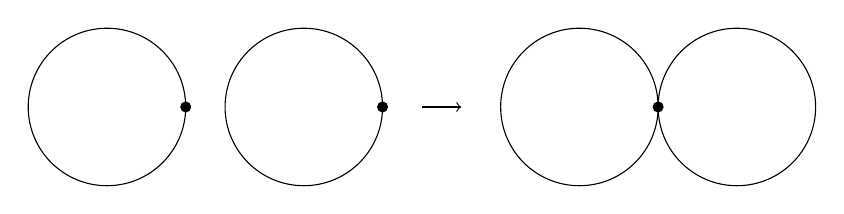
\begin{tikzpicture}
        \draw (-7,0) circle (1);
        \fill (-6,0) circle (2pt);
        \draw (-4.5,0) circle (1);
        \fill (-3.5,0) circle (2pt);
        \draw[->] (-3,0) -- (-2.5,0);
        \draw (-1,0) circle (1);
        \draw (1,0) circle (1);
        \fill (0,0)  circle (2pt);
    \end{tikzpicture}
.\] 
\end{example}

\begin{example}
    Es ist $[0,\frac{1}{2}] \twedge_{\frac{1}{2}} [\frac{1}{2},1] \cong [0,1]$. Verkleben wir allerdings die Punkte $\frac{1}{4}$ und $\frac{3}{4}$, so erhalten wir nicht das Einheitsintervall, sondern ein Plus-Zeichen.
\end{example}

\begin{remark*}
    Aus anderen mathematischen Richtungen kennt man das Wort 'Wedge' eigentlich als Symbol $\wedge$. In der Topologie ist dies jedoch anders. Das Symbol $\tsmash$ heißt 'Smash' und definiert das Smash-Produkt zweier Räume:
     \[
    X \land Y := X \times  Y / X \twedge Y
    .\]  
Es ist z.B. $S^1\tsmash S^1 \cong S^2$ und sogar allgemein $S^n \tsmash S^n \cong S^{2n}$.
\end{remark*}

\begin{gag}
\begin{definition}[Smash-Produkt]\label{def:smash-produkt}
    Seien $X,Y$ topologische Räume und  $x\in X, y\in Y$ Punkte. Dann ist das \vocab{Smash-Produkt} definiert als
    \[
        (X,x) \tsmash (Y,y) = X\times Y / (X\times \left \{y\right\} \cup \left \{x\right\} \times Y)
    .\] 
\end{definition}
\end{gag}


\missingfigure{Torus als Smash-Produkt $S^1 \tsmash S^1$}
\todo{Bruch-nummer hinzufügen}
%%%%%Für die Latex-Nutzer: Ich verwende die Befehle \twedge und \tsmash, um die topologischen wedge und smash- symbole zu erzeugen. Ich bin ein Fan von semantischen Commands, das ermöglich a) sich nicht verwirren zu lassen, wenn man TeXt, wenn man den Code wieder liest etc und vermeidet Konflikte mit anderen Definitionen bzw. Dateien (und verwirrt mich weniger). Außerdem hat es den Vorteil, dass ich jederzeit \twedge und \tsmash neu definieren kann, sollte es nötig sein. Die No tation ist etwas analog zu \land und \lor für 'logic and" und 'logic ar' etc.
\begin{remark*}
    In der Pause stellte sich die Frage, ob es ein Beispiel für einen nicht-normalen Hausdorff-Raum gibt. Siehe hierzu \cite[][Gegenbeispiel 86]{counterexamples}.
\end{remark*}

\begin{example*}[Punktierte Tychonoff-Planke]

    Wir geben (nach einem Kommentar von {\sc Melvin Weiß}) ein Beispiel für einen Hausdorff-Raum, der nicht normal ist, die sogenannte \vocab{gelöschte Tychonoff-Planke} (eng: 'deleted Tychonoff plank'). Sei hierzu $\aleph_0$ die erste unendliche Kardinalzahl und $\aleph_1$ die erste überabzählbare Kardinalzahl. Auf den Räumen $[0,\aleph_0]$ und  $[0,\aleph_1]$ können wir in natürlicher Weise eine Topologie definieren, indem wir die Anfangs- und Endstücke des Intervalls als Subbasis wählen. Der Raum
    \[
        T := [0,\aleph_0] \times [0,\aleph_1]
    .\] 
    heißt Tychonoff-Planke und ist ein kompakter Hausdorff-Raum, also insbesondere normal. Der Teilraum
    \[
        T_{\text{deleted}} := T \setminus \left \{\infty\right\}  := T \setminus \left \{(\aleph_0, \aleph_1)\right\} 
    .\] 
    heißt punktierte Tychonoff-Planke und ist ein lokal kompakter Hausdorffraum, allerdings nicht normal.
    \begin{proof}[Beweisskizze]
        Wir verweisen an dieser Stelle darauf, dass $[0,α]$ für jede Ordinalzahl  $α$ ein kompakter Hausdorffraum ist, das ganze beruht im Wesentlichen darauf, dass die Ordinalzahlen eine Wohlordnung bilden. Also ist  $T$ als produkt von kompakten Hausdorffräumen ebenfalls kompakter Hausdorffraum (\autoref{thm:produkte-von-Hausdorff-Räumen-sind-Hausdorff}, \autoref{thm:tychonoff}), also normal (\autoref{thm:kompakter-hausdorff-raum-ist-normal}. \\
        Der Teilraum $T_{\text{deleted}}$ ist also als Teilraum eines Hausdorff-Raumes ebenfalls Hausdorff. Allerdings lassen sich die beiden abgeschlossenen Mengen
        \[
            A:= [0,\aleph_0) \times \left \{\aleph_1\right\}, \qquad B := \left \{\aleph_0\right\} \times [0,\aleph_1)
        .\] 
        nicht durch offene Mengen trennen: \\
        Angenommen, wir finden $A\subset U$ und $B\subset V$ mit $U,V$ offen. Sei  $n\in \N = \aleph_0$ beliebig, dann ist $(n,\aleph_1)\in A\subset U$. Da $U$ offen, finden wir ein Basiselement der Produkttopologie, das  $(n,\aleph_1)$ enthält, also gibt es  $α_n<\aleph_1$, sodass bereits das Intervall  $\left \{n\right\} \times [α_n, \aleph_1] \subset U$ ist (an dieser Stelle sollte man sich eigentlich genauer Fragen, wie die Topologie auf einer Ordinalzahl definiert ist, die Details, und warum die behauptete Aussage folgt, sind aber leicht zu überlegen). Jetzt kommt der Trick: Wir betrachten
        \[
        β := \sup_{n\in \N} α_n
        .\] 
        \begin{claim}
            $β<\aleph_1$
        \end{claim}
        \begin{subproof}
            Es ist $β = \bigcup_{n\in \N} α_n$ (nach Konstruktion der Ordinalzahlen) wieder eine Ordinalzahl. Da $α_n < \aleph_1$ ist  $α_n$ (als Menge) abzählbar, und somit auch  $β$ als abzählbare Vereinigung abzählbarer Mengen, also ist auch  $β<\aleph_1$, weil  $\aleph_1$ überabzählbar ist.    
        \end{subproof}
        Jetzt wissen wir also, dass sogar der Streifen $[0,\aleph_0) \times [β,\aleph_1]\subset U$ ist (nach Wahl der $α_n$), d.h. die Menge  $U$ enthält sogar ein 'Rechteck positiver Höhe', was absurd ist. Formal können wir argumentieren, indem wir jetzt für den Punkt $(\aleph_0, β)\in B$ eine offene Umgebung wählen und somit ein Intervall $[\gamma, \aleph_0) \times \left \{β\right\} \subset V$ mit $\gamma <\aleph_0$ finden. Dann ist jedoch $(\gamma, \beta)\in U\cap V$, \contra.
    \end{proof}
        Das absurde an dem Beispiel ist, dass wir das Supremum der $α_n$ nehmen, die zwar alle  $<\aleph_1$ sind, aber dennoch  $β \neq \aleph_1$ folgt. Von den reellen Zahlen sind wir gewohnt, dass hier Gleichheit eintreten kann. Wir haben also sogar gezeigt, dass
        \begin{claim}
            Im Raum $[0,\aleph_1)$ konvergiert jede monoton steigende Folge.
        \end{claim}
        \noindent\textbf{obwohl} der Raum nach oben keine Schranke besitzt. Die Moral daran ist ungefähr '$\aleph_1$ ist zu groß, um von Folgen erreicht zu werden'. Das motiviert auch die Einführung von Netzen für größere topologische Räume, die wir hier aber nicht behandeln.
\end{example*}


Wir haben nun Abbildungen $j_i \colon X_i \to  X_1 \bigcup_{X_0} X_2 $:
\[
\begin{tikzcd}
    X_1 \ar[swap]{dr}{j_1} \ar{r}{ι_1}& X_1 \coprod X_2 \ar{d}{q} \\
        & X_1 \bigcup\limits_{X_0} X_2 
\end{tikzcd}
\qquad
\begin{tikzcd}
    X_2 \ar[swap]{dr}{j_2} \ar{r}{ι_2}& X_1 \coprod X_2 \ar{d}{q} \\
        & X_2 \bigcup\limits_{X_0} X_1 
\end{tikzcd}
.\] 
\begin{lemma}\label{lm:injektive-einbettung-ergibt-injetive-projektion-auf-koprodukt-über-basis}
Seien $X_0,X_1,X_2$ topologische Räume, $f_1 \colon X_0 \to  X_1$, $f_2 \colon X_0 \to  X_2$ stetig und betrachte die kanonischen Abbildungen $ι_i\colon X_i \to  X_1 \coprod X_2$ sowie $q : X_1 \coprod X_2 \to  X_1 \bigcup\limits_{X_0} X_2$. \\
Ist $f_1$ injektiv so ist $j_2$ injektiv. Ist  $f_2$ injektiv, so ist $j_1$ injektiv.
\end{lemma}
\begin{proof}
    Wir zeigen nur die erste Aussage, die zweite folgt aus Symmetriegründen. Seien $x,y \in X_2$ mit $j_2(x) = j_2(y)$, nach Konstruktion ist also $x \sim y$. Da die Äquivalenzrelation erzeugt ist von $f_1(x) \sim f_2(x)$, gibt es nun eine Folge von Punkten $x := p_1 \sim  p_2 \sim  \ldots \sim  p_n =: y$, die jeweils von der Form $f_1(x) \sim  f_2(x)$ sind.
    \begin{recap}
        Erzeugen wir eine Äquivalenzrelation durch $x_i \sim  y_i$ für $i\in I$, so sind zwei Element $x,y$ genau dann äquivalent, wenn es eine endliche Folge  $x = a_0 \sim  a_1 \sim  \ldots \sim a_n = y$ gibt, wobei $\left \{a_i, a_{i+1}\right\}  = \left \{(x_i, y_i\right\} $   für ein $i\in I$. 
    \end{recap}
    Genauer gibt es also $x_1\in X_0$ mit $f_2(x_1 ) = p_1 = x$ und $f_1(x_1) = p_2$, und $\exists x_2\in X_0$ mit $f_2(x_2) = p_3$ sowie $f_1(x_2) = p_2$ (auf welcher Seite $f_1$ bzw. $f_2$ steht, ergibt sich daraus, dass die Punkte $p_i$ alternierend aus  $X_1$,$X_2$ kommen müssen). Allgemein gibt es also $x_i \in X_0$ mit 
    \[
        f_2(x_{2i-1}) = p_{2i-1},\quad f_1(x_{2i-1} = p_{2i}),\quad  f_2(x_{2i} = p_{2i+1}),\quad f_1(x_{2i}) = p_{2i} 
    \]
    Nun wissen wir aber, dass $f_1$ injektiv ist, also ergibt sich $x_{2i-1} = x_{2i}$. Dann ist bereits:
    \[
        x = f_2(x_1) = f_2(x_2) = p_3 = = f_2(x_3) = f_2(x_4) = p_5 = \ldots = y
    .\] 
    und damit haben wir $x=y$ gezeigt und  $j_2$ ist wie gewünscht injektiv.
    \missingfigure{Beweisskizze}
\end{proof}

Wir kehren nun zu unserer Ausgangssituation bzw. Ausgangsfrage zurück: \\
Sei $X$ ein topologischer Raum und seien  $X_1,X_2\subset X$ Unterräume, sodass $X_1 \cup X_2 = X$. Setze $X_0 := X_1 \cap  X_2$. \\
Betrachte
    \begin{equation*}
    f': \left| \begin{array}{c c l} 
    X_1\coprod X_2 & \longrightarrow & X \\
    (1,x) & \longmapsto &  x \\
    (2,x) & \longmapsto & x
    \end{array} \right.
\end{equation*}
(im Wesentlichen ist das die Projektion, sodass wir das 'disjunkt' aus der Vereinigung wieder loswerden). Dann faktorisiert $f'$ nach der Universellen Eigenschaft der Quotiententopologie über $f: X_1 \bigcup_{X_0} X_2 \to  X$, dh wir erhalten:
\[
\begin{tikzcd}
    X_1 \coprod X_2 \ar{r}{f'} \ar[swap]{d}{q} & X \\
    X_1 \bigcup_{X_0} X_2 \ar[swap]{ur}{f} 
\end{tikzcd}
\]
Es ist $f'$ surjektiv wegen  $X_1 \cup X_2 = X$, also auch $f'$, und wir prüfen auch leicht die Injektivität von  $f$. Nun ist:

\begin{theorem}\label{thm:raum-ist-koprodukt-über-schnitt-zweier-teilmengen-wenn-diese-offen-oder-abgeschlossen-sind}
    Betrachte die Konstruktion von eben. Nimm an, dass zusätzlich eine der Bedingungen
     \begin{enumerate}[1.]
        \item $X_1,X_2$ sind offen.
        \item $X_1,X_2$ sind abgeschlossen.
    \end{enumerate}
    gilt. Dann ist $f$ ein Homöomorphismus.
\end{theorem}

\begin{proof}
Wir zeigen die Aussage nur unter Verwendung von 2., der Fall 1. geht analog. Es genügt zu zeigen, dass $f$ abgeschlossen ist (weil wir schon wissen, dass  $f$ eine stetige Bijektion ist). Sei  $A\subset X_1\bigcup\limits_{X_0} X_2$ abgeschlossen. Dann sind $j^{-1}_1(A)\subset X_1$ und $j^{-1}_2(A)\subset X_2$ abgeschlossen, da $j_1,j_2$ stetig. Wegen
    \[
        f(A) = j^{-1}_1(A) \cup j^{-1}_2(A)
    .\] 
    sind wir fertig, indem wir ($j^{-1}_1(A)\subset X_1$ abgeschlossen und $X_1\subset X$ abgeschlossen) $\implies j^{-1}_1(A) \subset X$ abgeschlossen bemerken. 
\end{proof}

\begin{remark*}
    Die Stetigkeit von $f^{-1}$ kann man auch mit \autoref{aufgabe-2.2} einsehen, weil $X = X_1 \cup X_2$ mit $X_1,X_2$ abgeschlossen ist, und die entsprechenden Teilabbildungen $X_1 \to X_1 \bigcup_{X_0} X_2$ Einbettungen sind. Im Wesentlichen wiederholen wir hier einfach nur die Aussage des Übungsblattes.
\end{remark*}

\begin{example}
    Sei $X = S^n$ und betrachte die Teilräume  \[
        X_1 = \left \{x\in S^n \mid  x_{n+1}\geq 0\right\} \qquad X_2 = \left \{x\in S^n \mid  x_{n+1} \leq 0\right\} 
    \]
    , also die obere und untere Halbkugel. Der Schnitt
    \[
    X_0 := X_1 \cap  X_2 = \left \{x\in S^n \mid  x_{n+1} = 0\right\} 
    .\] 
    ist dann genau der Äquator der Kugel, also lernen wir aus \autoref{thm:raum-ist-koprodukt-über-schnitt-zweier-teilmengen-wenn-diese-offen-oder-abgeschlossen-sind}, dass
     \[
    S^n \cong X_1 \bigcup_{X_0} X_2 
    .\] 
    Mit der Abbildung
        \begin{equation*}
        \begin{array}{c c l} 
        X_1 & \longrightarrow & D^n \\
        (x_1,\ldots,x_{n+1}) & \longmapsto &  (x_1,\ldots,x_n)
        \end{array}
    \end{equation*}
    (die Projektion auf die $n$-Dimensionale Scheibe) erhalten wir einen Homöomorphismus  $D^n \cong X_1, X_2$, also haben wir eigentlich sogar
    \[
    S^n \cong D^n \bigcup_{S^{n-1}} D^n
    .\] 
    gezeigt.
    \missingfigure{Kugel skizzieren}
    \begin{warning}
        Auch hier ist wieder wichtig, dass wir $S^{n-1}\hookrightarrow D^n$ jeweils kanonisch einbetten, für andere Abbildungen haben wir bereits gesehen, dass wir andere Räume erhalten können.
    \end{warning}
\end{example}





    \lecture[Markov-Ketten. Übergangsmatrizen.]{Mo 10 Mai 2021 10:15}{Markovketten}
\subsubsection{Markovketten (MK)}
\begin{itemize}
    \item Setze $X = (X_0,X_1,X_2,\ldots,X_n)$. Die Zeit beginnt hier bei $k=0$.
    \item Betrachte  $\Omega_k = \mathcal{S}$ für festes $\mathcal{S}$, also
        \[
            \Omega = \mathcal{S}^{n+1} = \left \{(x_0,\ldots,x_n) \mid  x_i \in \mathcal{S}, 0\leq i\leq n\right\} 
        .\] 
\end{itemize}

\begin{definition}[Markovkette]\label{def:markovkette}
    Eine \vocab{Markovkette} (abgekürzt: MK) ist ein mehrstufiges Modell mit der Eigenschaft
    \[
        p_k(x_k \mid  x_0,\ldots,x_{k-1}) = p_k (x_k\mid x_{k-1})
    .\] 
\end{definition}

\begin{question}
    Sei $\mathcal{S}$ abzählbar. Wie beschreibt man die Übergänge von $X_k$ nach  $X_{k+1}$?
\end{question}

\begin{definition}[Sotchastische Matrix]\label{def:stochastische-matrix}
    Eine Matrix $P = [\mathbb{P}(x,y)]_{x,y\in \mathcal{S}}$ mit den Eigenschaften
    \begin{enumerate}[label=\protect\circled{\alph*}]
        \item $\forall x\, \forall y \colon\mathbb{P}(x,y) \geq  0$
        \item $\forall x\in \mathcal{S}\colon\sum_{y\in \mathcal{S}} \mathbb{P}(x,y) = 1$
    \end{enumerate}
    heißt \vocab{stochastische Matrix}. 
\end{definition}

\begin{remark*}
    Beachte, dass die Matrix in obiger Definition nicht zwingend endlich sein muss, Definitionen verallgemeinern sich kanonisch. Wir fordern aber, dass $\mathcal{S}$ abzählbar ist.
\end{remark*}

\begin{lemma}\label{lm:übergangsmatrix-ist-stochastische-matrix}
    Die Matrix $P_k$ mit den Einträgen
    \[
        P_k(x,y) = p_k(Y \mid X) \quad \forall x,y,\in \mathcal{S}
    .\] 
    ist eine stochastische Matrix.
\end{lemma}

\begin{proof}
    Offenbar ist $p_k(Y\mid X) \geq 0$. Zudem
    \begin{IEEEeqnarray*}{rCl}
        \sum_{y\in \mathcal{S}} P_k(x,y) & =&  \sum_{y\in \mathcal{S}} \mathbb{P}(X_k = Y \mid  X_{k-1} = x) \\
                                         & = & \mathbb{P}\left(\bigcup_{y\in \mathcal{S}} \left \{X_k = y\right\} \mid X_{k-1} = x\right) \\
                                         & = &  \mathbb{P}(\Omega_k \mid  X_{k-1}=x) \\
                                         & = & 1
    \end{IEEEeqnarray*}
    weil es sich bei $\mathbb{P}(\cdot \mid  X_{k-1}= x)$ um eine Wahrscheinlichkeitsverteilung handelt, und $\mathcal{S} = \bigsqcup_{y\in \mathcal{S}} \left \{y\right\} $ eine disjunkte Vereinigung ist.
\end{proof}

\begin{remark}
    $P_k$ ist eine sogenannte \vocab{Übergangsmatrix}. Sie beschreibt den Übergang der Markovkette von $\Omega_k$ nach $\Omega_{k+1}$ 
\end{remark}

Die Massenfunktion einer Markovkette ist
 \[
     p(x_0,x_1,\ldots,x_n) = p_0(x_0) \cdot P_1(x_0,x_1) \cdot  \ldots \cdot  P_n(x_{n-1},x_n)
.\] 
wobei $p_0$ die sogenannte \vocab{Anfangsverteilung} ist.

\begin{remark}
    Falls $P_k = \mathbb{P}$, d.h. die Übergangsmatrixk hängt nicht von $k$ ab, dann heißt die Markovkette  (zeitlich) \vocab{homogen}. 
\end{remark}

\begin{remark}
    Seien $P,Q$ zwei stochastische Matrizen. Dann ist auch $P\cdot Q$ eine stochastische Matrix, wobei
    \[
        (    P\cdot Q) (x,y) = \sum_{z\in \mathcal{S}} P(x,z) \cdot  Q(z,y)
    .\] 
\end{remark}

\begin{question}
    Was ist
    \begin{enumerate}[1)]
        \item $\mathbb{P}(X_n = x)$
        \item $\lim_{n\to \infty} \mathbb{P}(X_n = x)$ (Existiert dieser überhaupt?)
        \item Ist $\lim_{n \to \infty} \mathbb{P}(X_n = x)$ von $x_0$ abhängig?
    \end{enumerate}
\end{question}

\begin{theorem}[Massenfunktion in Markovketten]\label{thm:massenfunktion-einer-zufallsvariable-in-markovkette}
    Sei $μ_0$ der Zeilenvektor mit Elementen  $p_0(x), x\in \mathcal{S}$. Seien dazu $P_1,P_2,\ldots,P_n$ die Übergangsmatrizen einer Markovkette $X = (X_0,X_1,\ldots,X_n)$ auf $\mathcal{S}$. Dann hat die Wahrscheinlichkeit von $X_n$ die Massenfunkiton
    \[
        μ_n(x) := \mathbb{P}(X_n = x) = (μ_0 \cdot  P_1 \cdot  \ldots \cdot  P_n)(x) \quad \forall x\in \mathcal{S}
    .\] 
\end{theorem}

\begin{proof}
    \begin{IEEEeqnarray*}{rCl}
        \mathbb{P}(X_n = x) &=& \sum_{x_0,\ldots,x_{n-1}\in \mathcal{S}} \mathbb{P}(X_0 = x_0, \ldots, X_{n-1}=x_{n-1}, X_n = x) \\
                            & = & μ_0(x_0) P_1(x_0,x_1) \ldots P_n(x_{n-1},x)
    \end{IEEEeqnarray*}
\end{proof}

\begin{example}
    \begin{enumerate}[label=\protect\circled{\alph*}]
        \item Produktmodelle sind Markovketten.
        \item Irrfahrten (eng: 'Random Walk') auf $\Z^d$ sind Markovketten:\\
            Sei $\mathcal{S} = \Z^d$ mit $d\in \N$ fest. Die (symmetrische) Irrfahrt ist eine homogene Markovkette mit 
            \[
                P_k(x,y) = P(x,y) = \begin{cases}
                    \frac{1}{2d} & \text{falls } \lVert x-y \rVert =1 \\
                                0 & \text{sonst}
                \end{cases}
            .\] 
In jedem Schritt bewegen wir uns also auf einen benachbarten Gitterpunkt.
\item \vocab{Urnenmodell von Ehrenfest}. Wir haben ein System mit $N$ Teilchen, die auf zwei Urnen  $A,B$ verteilt sind. Zu jedem Zeitpunkt  $t\in \N$ welchselt eine zufällig ausgewählte Kugel die Urne. \\
    In der Makroskopischen Modellierung sei $n_A := \# \text{Teilchen in A}$. Dann ist
    \[
    \rho_A := \frac{n_A}{N}\in \left \{0,\frac{1}{N}, \ldots, \frac{N-1}{N},1\right\}  = : \mathcal{S}
    .\] 
    und die Markovkette, die die Zeitentwicklung von $\rho_A$ beschreibt, hat die Übergangsmatrix
     \[
         P(x,y) = \begin{cases}
             x & \text{falls } y = x-\frac{1}{N} \\
             1-x & \text{falls } y = x+\frac{1}{N} \\
             0 & \text{sonst}
         \end{cases}
    .\] 
    Die Fälle spiegeln wieder, dass wir ein Teilchen aus $A$ bzw.  $B$ gezogen haben, wobei der dritte Fall dijenigen  $y$ abdeckt, die wir nicht erreichen können, weil sich  $n_A$ immer nur um $\pm_1$ ändert. \\
    In der Mikroskopischen Modellierung nummerieren wir die Teilchen, d.h.
     \[
         \mathcal{S} = \left \{0,1\right\} ^n = \left \{σ = (σ_1, \ldots,σ_N) \mid  σ_k \in \left \{0,1\right\} , 1\leq k\leq N\right\} 
    .\] 
    wobei
    \[
    σ_k = \begin{cases}
        1 & \text{falls Teilchen } k \text{ ist in $A$}\\
        0 & \text{falls Teichen $k$ ist in  $B$}
    \end{cases}
    .\] 
    Die Dynamik von $σ\in \mathcal{S}$ wir durch die Markovkette beschrieben:
    \[
        P(σ,\tilde{σ}) = \begin{cases}
            \frac{1}{N} & \text{falls } \sum_{k=1}^N \abs{σ_k - \tilde{σ}_k} = 1 \\
            0 & \text{sonst}
        \end{cases} 
    .\] 
    \begin{remark}
        Die Notation $\sum_{k=1}^N \abs{σ_k - \tilde{σ_k} } =1$ ist nur eine kurze (elegante) Möglichkeit auszudrücken, dass sich $σ_k$ nach  $\tilde{σ}_k$ in nur einem Eintrag ändert.
    \end{remark}
    Es ergibt sich also eine Irrfahrt auf dem Hyperwürfel $\left \{0,1\right\} ^N$.
    \end{enumerate}
\end{example}

\begin{question}
    Was ist $P(X_l = y \mid X_k = x)$ für $k<l$ beliebig?
\end{question}

Intuitiv sollten wir hier $P_{k+1}\cdot \ldots\cdot P_l(x_k,x_l)$ erhalten, indem wir die Übergangsmatrizen multiplizieren.
\begin{theorem}[Markoveigenschaft]\label{thm:markov-eigenschaft}
    Sei $X$ eine Markovkette auf  $\mathcal{S}$. Für alle $0\leq k\leq l\leq n$ und $x_0,\ldots,x_l\in \mathcal{S}$ mit $\mathbb{P}(X_0 = x_0, \ldots, X_k = x_k) \neq 0$ ist
    \begin{equation}
        \begin{split}
            \mathbb{P}(X_l = x_l \mid  X_0 = x_0,\ldots,X_k = x_k) &= \mathbb{P}(X_l = x_l \mid  X_k = x_k) \\
                                                                   &= (P_{k+1}\cdot \ldots\cdot P_l)(x_k,x_l)
        \end{split}
    \end{equation}
    Diese Eigenschaft (erstes Gleichheitszeichen) heißt auch \vocab{Markov-Eigenschaft}. 
\end{theorem}

\begin{proof}
Es ergibt sich
\begin{IEEEeqnarray*}{Cl}
&    P(X_l = x_l \mid  X_0 = x_0, \ldots, X_k = x_k)\\
\stackrel{\text{Def.}}{=} &  \frac{P(X_0 = x_0, \ldots, X_k = X_k, X_l = x_l)}{P(X_0 = x_0, \ldots, X_k = X_k)} \\
= & \frac{\sum_{\substack{ x_{k+1},\ldots,x_{l-1} \\ x_{l+1},\ldots,x_n \in \mathcal{S}}} p_0(x_0) P_1(x_0,x_1) \cdot  \ldots \cdot P_k(x_{k-1},x_k) \cdot  P_{k+1}(x_k,x_{k+1})\cdot \ldots\cdot P_l(x_{l-1},x_l) \cdot P_{l+1}(x_l, x_{l+1}) \cdot  \ldots \cdot P_(x_{n-1},x_n)}{\sum_{x_{k+1},\ldots,x_n\in \mathcal{S}} \text{analog}} \\
= & \frac{\sum_{x_{k+1},\ldots,x_{l-1}\in \mathcal{S}} p_0(x_0)\cdot \ldots\cdot P_k(x_{k-1},x_k)\cdot P_{k+1}(x_1,x_{k+1})\cdot P_l(x_{l-1},x_l)}{p_0(x_0)\cdot \ldots\cdot P_k(x_{k-1},x_k)} \\
= & \sum_{x_{k+1},\ldots,x_{l-1}\in \mathcal{S}} P_{k+1}(x_{k},x_{k+1}) \cdot P_{l(x_{l-1},x_{l}}) \\
= & (P_{k+1}\cdot \ldots\cdot P_l) (x_k,x_l)
\end{IEEEeqnarray*}
Das zeigt die erste Gleichheit. Dazu ist
\begin{IEEEeqnarray*}{Cl}
    &\mathbb{P}(X_l = x_l \mid X_k = x_k) \\
    = &\frac{\mathbb{P}(X_l = x_l,X_k = x_k)}{\mathbb{P}(X_k = x_k)} \\
    = & \frac{\sum_{x_{k+1},\ldots,x_{l-1}\in \mathcal{S}} (μ_0 P_1\ldots P_k)(x_k)\cdot P_{k+1}(x_k,x_{k+1}\cdot P_l(x_{l-1},x_l)}{(μ_0 P_1\cdot \ldots\cdot P_k)(x_k)} \\
    = & (P_{k+1}\cdot \ldots\cdot P_l) (x_k,x_l)
\end{IEEEeqnarray*}
\end{proof}
\begin{example}
    Ist $\mathcal{S} = \left \{1,\ldots,N\right\}$, so ergibt sich mit $μ_0 = (μ_0(1), \ldots, μ_0(N))$ \ldots
    \[
        = (\sum_k μ_0(k) P(k,1), \sum_k μ_0(k) P(k,2),\ldots) = ((μP)(1), (μ_0P)(2), \ldots)
    .\] 
\end{example}
\todo{Beispiel fertig}

    \lecture[Beweis des Lemmas von Urysohn. Urysohn für beliebige Intervalle. Satz von Tietze. 'Quetschen' von stetigen Funktionen auf normalen Räumen. Beweis des Satz von Tietze. Metrisierungssatz von Urysohn.]{Di 18 Mai 2021 12:20}{Urysohn, Tietze}
Wir erinnern uns daran, dass wir gerade dabei waren, \autoref{thm:urysohn} zu beweisen.
\begin{lemma}\label{trennung-von-mengen-in-normalem-raum-für-urysohn-lemma}
    Sei $X$ ein normaler Raum,  $A\subset X$ abgeschlossen und $U\subset X$ offen mit  $A\subset U$. Dann existiert $V\subset X$ offen mit
    \[
    A\subset V\subset \overline{V}\subset U
    .\] 
\end{lemma}
\begin{figure}[ht]
    \centering
    \incfig{trennung-von-abgeschlossenen-mengen-durch-offene-in-normalem-raum}
    \caption{Skizze zu \autoref{trennung-von-mengen-in-normalem-raum-für-urysohn-lemma}}
    \label{fig:trennung-von-abgeschlossenen-mengen-durch-offene-in-normalem-raum}
\end{figure}
\begin{proof}
    Wegen $U$ offen ist  $X\setminus U$ abgeschlossen. Wegen $X$ normal gibt es  $V,V'$ offen mit  $A\subset V$ und $(X\setminus U)\subset V'$ mit $V\cap V'=\emptyset$. Nun ist
    \[
    A\subset V\subset X\setminus V' \subset U
    .\] 
    nach Definition des Abschlusses ist nun $A\subset V\subset \overline{V} \subset X\setminus V' \subset U$.
\end{proof}

\begin{proof}[Beweis von \autoref{thm:urysohn} (\nameref{thm:urysohn})]
    \begin{goal}
        $\forall r\in \Q\cap [0,1]$ konstruiere $V_r \subset X$ offen, sodass
         \begin{enumerate}[1.]
            \item $A\subset V_0$
            \item $B\subset X\setminus V_1$
            \item  $r<r' \implies \overline{V_r}\subset V_{r'}$
        \end{enumerate}
    \end{goal}
Dies genügt, denn dann wissen wir mit \autoref{lm:stetige-abbildung-durch-familie-von-rationalen-offenen-mengen}, dass 
\begin{IEEEeqnarray*}{rCl}
    \exists f: X &\to & [0,1] \text{ stetig} \\
        f(x) & = & 0 \quad \forall x\in V_0 \supset A
        \\ f(x) & = & 1 \quad \forall x \in  X \setminus V_1\supset B
\end{IEEEeqnarray*}
Wähle hierzu eine Abzählung $p_1,p_2,\ldots$ von $\Q\cap [0,1]$, sodass $p_1 = 1$ und $p_2 = 0$. Definiere nun $\left \{V_r\right\} $ rekursiv, wobei wir auch induktiv die Invariante erhalten wollen, dass $r<r' \implies \overline{V_r} \subset V_{r'}$.
\begin{itemize}
    \item $p_1 = 1$. Setze $V_1 \coloneqq X\setminus B$ (offen, weil $B$ abgeschlossen ist)
    \item  $p_2 = 0$. Nach \autoref{trennung-von-mengen-in-normalem-raum-für-urysohn-lemma} mit $A = A$ und  $U = X\setminus B$ finden wir $V_0$ offen mit 
        \[
        A\subset V_0 \subset \overline{V}_0 \subset X\setminus B =: V_1
        .\] 
    \item Sei $n\geq 3$, dann sind also $V_{p_1},V_{p_2},\ldots,V_{p_{n-1}}$ schon definiert. Es ist $\left \{p_1,p_2,\ldots,p_n\right\} $ wohlgeordnet, weil es sich um eine endliche Menge handelt, also gibt es unter ihnen einen direkten Vorgänger $p_i$ von  $p_n$, und einen direkten Nachfolger  $p_j$ von  $p_n$.
         \begin{recap}
            Es könnte z.B.  $n=5$ sein mit \\
            \begin{tabular}{c | c | c | c | c}
                $p_1$ & $p_2$ & $p_3$ & $p_4$ & $p_5$ \\
                1 & 0 & $\frac{1}{2}$ & $\frac{8}{9}$ & $\frac{3}{5}$
            \end{tabular} 
            Dann ist die Menge als $\left \{0,\frac{1}{2},\frac{3}{5},\frac{8}{9},1\right\} $ geordnet, und wir sehen $p_i = = \frac{1}{2} < \frac{3}{5} < \frac{8}{9} = p_j$.
        \end{recap}
        Verwende nun \autoref{trennung-von-mengen-in-normalem-raum-für-urysohn-lemma} mit $A = \overline{V_{p_i}}$ und $U = V_{p_j}$, (hier ist wichtig, dass wegen $p_i < p_j$ beretis  $\overline{V_{p_i}}\subset V_{p_j}$ gilt, sonst können wir das Lemma nicht anwenden.) \\
        Also finden wir $V$ mit  $\overline{V_{p_i}} \subset V \subset \overline{V} \subset V_{p_j}$. Man prüft leicht, dass wir so auch die Invariante der Induktion erhalten haben.
\end{itemize}
Also haben wir wie gewünscht die $V_i$ gefunden, und somit unsere Funktion.
\end{proof}

\begin{corollary}[Urysohn mit beliebigem Intervall]\label{cor:urysohn-mit-beliebigem-intervall}
    Sei $X$ ein normaler Raum und seien  $A,B\subset X$ disjunkt und abgeschlossen, sowie $a\leq b\in \R$ beliebig. Dann 
    \begin{IEEEeqnarray*}{rCl}
        \exists f: X & \to  & [a,b] \\
        f(A) & = &\left \{a\right\}  \\
        f(B) & = & \left \{b\right\} 
    \end{IEEEeqnarray*}
\end{corollary}

\begin{proof}
    Zunächst verwenden wir Urysohn, um eine stetige Funktion $g: X \to  [0,1]$ zu erhalten mit $f(A) = \left \{0\right\} $ und $f(B) = \left \{1\right\}$, dann verknüpfen wir mit der stetigen Abbildung
        \begin{equation*}
        h: \left| \begin{array}{c c l} 
            [0,1] & \longrightarrow & [a,b] \\
            t & \longmapsto &  (1-t)a + tb
        \end{array} \right.
    \end{equation*}
    und wir erhalten sofort die gewünschten Eigenschaften, indem wir $f = h \circ  g$ setzen.
\end{proof}

\section{Der Erweiterungssatz von Tietze}
Wir sehen jetzt das \nameref{thm:urysohn} in Action:
\begin{theorem}[Erweiterungssatz von Tietze]\label{thm:tietze}
    Sei $X$ ein normaler Raum und  $A\subset X$ abgeschlossen. Jede stetige Funktion $f: A \to  [-1,1]$ lässt sich fortsetzen zu einer stetigen Funktion $\overline{f}: X \to  [-1,1]$, d.h. $\overline{f}\mid _{A} \equiv f$.
\end{theorem}

\begin{remark}
    Das Urysohn'sche Lemma ist ein Spezialfall des \nameref{thm:tietze}: \\
    Sei $X$ normal und  $B,C\subset X$ abgeschlossen, disjunkt. Dann betrachte die Funktion
        \begin{equation*}
        f: \left| \begin{array}{c c l} 
            B\cup C & \longrightarrow & [-1,1] \\
        B & \longmapsto &  -1 \\
        C & \longmapsto & 1
        \end{array} \right.
    \end{equation*}
    \begin{question}
        Gibt es eine Fortsetzung $\overline{f}: X \to  [-1,1]$?
    \end{question}
    Für jede solche Fortsetzung muss auch  $\overline{f}\mid _{B} = f$, also $\overline{f}(B) = -1$ und $\overline{f}(C) =1$ gelten, also genau das, was wir von Urysohn fordern. \\
    Allerdings sagt uns der \nameref{thm:tietze} genau, dass wir solche eine Fortsetzung finden.
\end{remark}

\begin{proof}[Beweis von \autoref{thm:tietze} (\nameref{thm:tietze})]
    \label{proof:tietze1}
    \begin{strategy}
        Wir konstruieren eine Folge stetiger Funktionen \\
        $\left \{s_n : X \to  [-1,1]\right\}_{n\geq 1}$, sodass
        \begin{enumerate}[(i)]
            \item $\left \{s_n\right\} $ konvergiert \vocab[Konvergenz!gleichmäßige]{gleichmäßig} gegen eine Funktion $s: X \to  [-1,1]$, d.h. für jedes $ε>0$ existiert  $N\in \N$, sodass 
                \[
                \emphasize{\forall} x \in X,n\geq N \colon\qquad    d(s_n(x), s(x))<ε
                .\] 
                Weil $\left \{s_n\right\} $ gleichmäßig konvergiert, ist $s$ stetig (Übungsblatt 5, Aufgabe 3 (iv)).
            \item  $s\mid _{A} = f$
        \end{enumerate}
    \end{strategy}
    Dazu benötigen wir erstmal einige Lemmata, die wir im folgenden erarbeiten.
\end{proof}

\begin{lemma}\label{lm:kompression-von-funktionen-auf-abgeschlossenen-mengen-in-normalem-raum}
    Sei $X$ normal und  $A\subset X$ abgeschlossen. Sei $\alpha : A \to  [-r,r]$ für $r\in \R_{\geq 0}$ stetig. Dann existiert $g: X \to  \left[ -\frac{1}{3}r, \frac{1}{3}r \right]$ stetig mit $\abs{α(a) - g(a)} \leq  \frac{2}{3}r $ für $a\in A$.
\end{lemma}
\begin{proof}
    Setze $B \coloneqq α^{-1}\left(\left[ -r,-\frac{1}{3}r \right]\right)$ und $C\coloneqq α^{-1}\left(\left[ \frac{1}{3}r,r \right]\right)$. Wegen $α$ stetig sind  $B,C$ abgeschlossen, und sie sind auch disjunkt, weil die Intervalle disjunkt sind. Nach \nameref{cor:urysohn-mit-beliebigem-intervall} finden wir also eine stetige Funktion
    \begin{IEEEeqnarray*}{rCl}
        g: X & \to  & \left[ -\frac{1}{3}r, \frac{1}{3}r \right] \\
        g(B) & = & \left \{-\frac{1}{3}r\right\} \\ 
        g(C) & = & \left \{\frac{1}{3}r\right\} 
    \end{IEEEeqnarray*}
    \begin{tikzpicture}
        \draw (0,-0.2) -- (8,-0.2) node[anchor = west] {$X$};
        \foreach \x in {0,1,2,3} {
            \draw[red,thick,dotted] (0,\x) -- (8,\x);
        }
        \draw (0,0) node[anchor=east] {$-r$};
        \draw (0,1) node[anchor=east] {$-\frac{1}{3}r$};
        \draw (0,2) node[anchor=east] {$\frac{1}{3}r$};
        \draw (0,3) node[anchor=east] {$r$};
        \draw[green!60!black, line width = 2pt] (4,-0.2) -- (5,-0.2) node[midway,anchor=north] {$B$};
        \draw[orange!90!black, line width = 2pt] (1,-0.2) -- (2,-0.2) (2.9,-0.2) -- node[midway, anchor = north] {$C$} (3.5,-0.2) (6,-0.2) -- (7,-0.2);
        \draw[line width = 1.5pt,blue] (1,-0.1) -- (1,-0.3);
        \draw[line width = 1.5pt,blue] (7,-0.1) -- (7,-0.3);
        %Graph of alpha
        \draw[blue!70!white,thick] (1,3) to[out = 0, in = 100] (2,2) to[out = -80, in = 180] (2.6,1.6) to[out = 0, in = 210] (2.9,2) to [out = 30,in=180] (3.1,2.4) to[out = 0,in = 120] (3.5,2) to[,out = -60,in = 100] (4,1) to[out = -80, in = 180] (4.5,0.2) to[out=0, in =240] (5,1) to[out = 60, in = 250] (6,2) to[out =70, in = 180] (6.5,3) to[out = 0, in = 130] node[near end, anchor = south west]{$α$} (7,2);
        %Graph of corresponding g:
        \draw[red, thick] (0.2,0.5) to[in = 230] node[near start, anchor = north west] {$g$} (1,2);
        \draw[red, thick] (2,2) to[out = -70, in = 180] (2.3,1.5) to[out = 0, in = 210] (2.9,2);
        \draw[red, thick] (3.5,2) to[out = -30, in = 130] (4,1);
        \draw[red, thick] (5,1) parabola (6,2);
        \draw[red, thick] (7,2) to[out = -40, in = 180] (7.5,1.3) to[out = 0, in = 250] (8,2.8);
        \draw[red, line width = 1.5pt] (4,1) -- (5,1);
        \draw[red, line width = 1.5pt] (1,2) -- (2,2) (2.9,2) -- (3.5,2) (6,2) -- (7,2);
        \draw[decorate, decoration={brace,mirror,amplitude=4pt}, yshift = -20pt, blue] (1,0) -- (7,0) node[midway, anchor = north, yshift = -5pt] {$A$};
    \end{tikzpicture}
    \begin{claim}
        $g$ erfüllt die Bedingungen unseres Lemmas, d.h.  
        \[
        \abs{α(a) - g(a) } \leq \frac{2}{3}r \qquad \forall a\in A
        .\] 
    \end{claim}
    \begin{subproof}
        \begin{itemize}
            \item Sei $a\in B$, Dann ist $α(a) \in \left[ -r, -\frac{1}{3}r \right]$ und $g(a) = -\frac{1}{3}r$, also gilt die Ungleichung.
            \item Sei $a\in C$. Dann ist $α(a) \in \left[ \frac{1}{3}r,r \right]$ und $g(a) = \frac{1}{3}r$, also, also gilt die Ungleichung.
            \item Sei $a\in A \setminus (B\cup C)$. Dann ist $α(a),g(a) \in \left[ -\frac{1}{3}r,\frac{1}{3}r \right] $, und damit ist der Abstand auch höchstens $\frac{2}{3}r$.
        \end{itemize}
    \end{subproof}
\end{proof}
\begin{remark*}
    In der Vorlesung kam die Frage auf, ob wir manche der gerade bewiesenen Resultate auch auf die Analysis übertragen können, indem wir z.B. den Fixpunktsatz von Banach anwenden.
\end{remark*}
\todo{darüber nachdenken}

\begin{proof}[Fortsetzung des Beweises des \nameref{thm:tietze}]
    Definiere die Folgen $s_n$ induktiv. Dazu \\
    \underline{Schritt 1}: Verwende \autoref{lm:kompression-von-funktionen-auf-abgeschlossenen-mengen-in-normalem-raum} mit $α = f$ und  $r = 1$, also erhalten wir
    \[
    g_1 : X \to  \left[ -\frac{1}{3}r, \frac{1}{3}r \right] 
    .\] 
    settig mit $\abs{f(a) - g(a)} \leq \frac{2}{3}$ für jedes $a\in A$. Setze $s_1 = g_1$. \\
    \underline{Induktionsschritt} Angenommen, wir haben schon stetige Funktion $g_1,\ldots,g_n$ auf $X$ mit
    \[
        g_i : X \to  \left[ -\left( \frac{2}{3} \right) ^{i-1}\cdot \frac{1}{3}, \left( \frac{2}{3} \right) ^{i-1}\cdot \frac{1}{3} \right] 
    .\]
    und 
    \[
        \abs{f(a) - \sum_{i=1}^n g_i(a)} \leq  \left( \frac{2}{3} \right) ^n \qquad \forall a\in A 
    .\] 
    Verwende nun wieder \autoref{lm:kompression-von-funktionen-auf-abgeschlossenen-mengen-in-normalem-raum} mit $α = f- \sum_{i=1}^n g_i\mid _{A}$ und $r = \left( \frac{2}{3} \right) ^n$. \\
    Es gibt also
    \[
        g_{n+1} \colon X \to  \left[ -\frac{1}{3}\cdot \left( \frac{2}{3} \right) ^{n}, \frac{1}{3}\cdot \left( \frac{2}{3} \right) ^n \right] 
    .\] 
    Wir erhalten nun
    \begin{IEEEeqnarray*}{rCl}
        \abs{f(a) - \sum_{i=1}^n g_i(a) - g_{n+1}(a)} & = &  \abs{f(a) - \sum_{i=1}^{n+1} g_i(a)}   \\
                                                      & \leq  & \frac{2}{3}\cdot \left( \frac{2}{3} \right) ^n = \left( \frac{2}{3} \right) ^{n+1}
    \end{IEEEeqnarray*}
    Nun definiere
    \[
    s_{n+1} \coloneqq \sum_{i=1}^{n+1} g_i : X \to \R
    .\] 
    \begin{claim}
        $s_n$ hat Bild in $[-1,1]$ für jedes  $n\in \N$.
    \end{claim}
    \begin{subproof}
        \begin{IEEEeqnarray*}{rCl}
            \abs{s_n(x)} & =&   \abs{\sum_{i=1}^n g_i(x)} \leq  \sum_{i=1}^n  \abs{g_i(x)} \\
                         & \leq& \sum_{i=1}^n \left( \frac{2}{3} \right) ^{i-1}\cdot \frac{1}{3}  \\
                         & \leq  & \sum_{i=1}^{\infty} \left( \frac{2}{3} \right) ^{i-1}\cdot \frac{1}{3}  \\
                         & = & \frac{\frac{1}{3}}{1-\frac{2}{3}} = 1
        \end{IEEEeqnarray*}
        Die andere Schranke zeigt man völlig analog.
    \end{subproof}
    \begin{claim}
        Die Folge $\left \{s_n\right\} _{n\in \N}$ konvergiert gleichmäßig gegen $s$.
    \end{claim}
    \begin{subproof}
        Für $k>n$ ist 
         \begin{IEEEeqnarray*}{rCl}
             \abs{s_k(x) - s_n(x)} & = & \abs{ \sum_{i=n+1}^k g_i(x) } \\
                                   & \leq  & \sum_{i=1}^{n+1} \frac{1}{3}\cdot \left( \frac{2}{3} \right) ^{i-1} \\
                                   & = &  \sum_{i=n+1}^{\infty} \frac{1}{3}\cdot \left( \frac{2}{3} \right) ^{i-1} \\
                                   & = & \frac{1}{3}\cdot \frac{\left( \frac{2}{3} \right) ^n}{1-\frac{2}{3}} \\
                                   & = &\left( \frac{2}{3} \right) ^n
        \end{IEEEeqnarray*}
        \begin{enumerate}[(i)]
            \item Für jedes $x\in X$ ist $\left \{s_n(x)\right\}_{n\geq 1} $ eine Cauchy-Folge, also konvergiert sie zu einem Punkt $s(x) \in [-1,1]$.
            \item Intuitiv reicht es für gleichmäßige Stetigkeit schon zu sehen, dass in obiger Abschätzung kein $x$ vorkommt. Genauer: \\
                Sei  $ε>0$, so  $\exists  N \in \N$ mit $\forall n > N \implies \left( \frac{2}{3} \right) ^n < ε$. Dann ist
                \begin{IEEEeqnarray*}{rCl}
                    \abs{s(x) - s_n(x)} & = & \abs{\lim_{k \to \infty} s_k(x) - s_n(x)} \\
                                        & = & \lim_{k \to \infty} \abs{s_k(x) - s_n(x)} \\
                                        & \leq  & \left( \frac{2}{3} \right) ^n \\
                                        & < &ε
                \end{IEEEeqnarray*}
                also ist die Konvergenz gleichmäßig, und $s$ ist stetig.
        \end{enumerate}
    \end{subproof}
    Setze nun $\overline{f} \coloneqq s$, dann überprüfen wir
    \begin{claim}
        $\overline{f}$ ist eine Fortsetzung von $f$, d.h.  $\overline{f}\mid _{A} = f$.
    \end{claim}
    \begin{subproof}
        Es ist 
        \begin{IEEEeqnarray*}{rCl}
            \abs{f(a) - s_n(a)} = \abs{f(a) - \sum_{i=1}^n g_i(a)} \leq  \left( \frac{2}{3} \right) ^n  
        \end{IEEEeqnarray*}
        also 
        \begin{IEEEeqnarray*}{rCl}
            \lim_{n \to \infty} \abs{f(a) - s_n(a)} \leq  \lim_{n \to \infty}  \left( \frac{2}{3} \right) ^n = 0
        \end{IEEEeqnarray*}
        Also ist 
        \[
            s(a) \coloneqq  \lim_{n \to \infty} s_n(a) = f(a)
        .\] 
        für jedes $a\in A$.
    \end{subproof}
    Wir haben also eine Fortsetzung gefunden, und sind damit fertig.
\end{proof}

\begin{corollary}[Version des Satzes von Tietze]\label{cor:tietze-2}
    Sei $X$ ein normaler Raum und  $A\subset X$ abgeschlossen. Dann gilt folgendes:
    \begin{enumerate}[1.]
        \item Jede stetige Funktion $f: A \to  [a,b]$ lässt sich zu einer Funktion $\overline{f} : X \to  [a,b]$ fortsetzen.
        \item Jede stetige Funktion $f: A \to  \R$ lässt sich fortsetzen zu einer Funktion $\overline{f}\colon X \to \R$.
    \end{enumerate}
\end{corollary}
\begin{proof}
    Übung.
\end{proof}


\section{Der Metrisierungssatz von Urysohn}
\begin{theorem}[Metrisierungssatz von Urysohn]\label{thm:metrisierungsssatz-von-urysohn}
    Jeder normale Raum mit abzählbarer Basis der Topologie ist metrisierbar.
\end{theorem}
\begin{proof}
    \begin{strategy}
        \underline{Schritt 1}: Betrachte $\prod_{\N} [0,1]$ in der Produkttopologie und zeige, dass der Raum emtrisierbar ist. Dieser Raum heißt \vocab{Hilbert-Würfel}.  \\
        \underline{Schritt 2}: Sei $X$ normal mit abzählbarer Basis, wir zeigen, dass wir eine Einbettung  $F : X \to  \prod_{\N} [0,1]$ finden.
        Dann sind wir fertig, da 
        \[
            X \cong F(X) \subset \prod_{\N}[0,1]
        .\] 
        ein Unterraum eines metrischen Raumes ist.
    \end{strategy}
\end{proof}

    % end lectures
    \printindex
    \newpage
    \thispagestyle{plain}
    \printbibliography
    \addcontentsline{toc}{section}{Literatur}
\end{document}
